\documentclass[a4paper, 11pt]{article}

\usepackage[utf8]{inputenc}
\usepackage[T1]{fontenc}
\usepackage[english]{babel}
\usepackage{enumitem}
\usepackage{amsthm, amsmath, amssymb, amsfonts, mathtools, mathrsfs}
\usepackage{graphicx, calc}
\usepackage{empheq}
\usepackage{geometry}
\geometry{a4paper, left = 20mm, right = 20mm, top = 30mm, bottom = 30mm}
\usepackage{xspace}
\usepackage{relsize}
\usepackage{fancyhdr}
\usepackage{pdflscape}
\usepackage{csquotes}
\usepackage{titling}
\usepackage{accents}
\usepackage[labelfont=bf,labelsep=period]{caption}
\usepackage{subcaption}
\usepackage{placeins} % FloatBarrier
\usepackage{physics}
\usepackage{tikz,tikz-3dplot}
\usetikzlibrary{patterns,decorations,decorations.markings}
\usepackage{lmodern}
\usepackage{xcolor}
\usepackage{booktabs}
\usepackage{chngcntr}
\usepackage{algorithm}
\usepackage{algorithmicx}
\usepackage{algpseudocode}
\usepackage[sorting=none, style=numeric]{biblatex}
\addbibresource{references.bib}


\usepackage{hyperref}
\hypersetup{
	colorlinks,
	citecolor=green,
	filecolor=black,
	linkcolor=blue,
	urlcolor=blue
}


\pagestyle{fancy}
\fancyhf{}
\setlength{\headheight}{30pt}
\lhead{Numerical Solution of the Convection--Diffusion Equations}
\rhead{ESEIAAT 2020--2021}
\cfoot{\thepage}

\setlength{\parskip}{0.2cm}%

% Comandos
\newcommand{\n}{\mathbb{N}}
\newcommand{\z}{\mathbb{Z}}
\newcommand{\q}{\mathbb{Q}}
\renewcommand{\real}{\mathbb{R}}
\newcommand{\cplex}{\mathbb{C}}
\renewcommand{\k}{\mathbb{K}}
\newcommand{\car}[1]{\mathrm{char}\left(#1\right)}
\newcommand{\class}[1]{\overline{#1}}
\newcommand{\mcd}[1]{\mathrm{mcd}{#1}}
\renewcommand{\mod}[1]{\ (\mathrm{mod}\ #1)}
\newcommand{\fractions}[1]{\mathrm{Fr}(#1)}
\renewcommand{\gcd}[1]{\mathrm{mcd} #1}
\newcommand{\mcm}[1]{\mathrm{mcm} #1}
\newcommand{\conj}[1]{\overline{#1}}
\newcommand{\prob}[1]{p \left( #1 \right)}
\newcommand{\esp}[1]{\mathbb{E} \left[ #1 \right]}
\newcommand{\scr}[2]{\left\langle #1, #2 \right\rangle}
\newcommand{\Int}{\int\limits}
\newcommand{\id}{\mathrm{Id}}
\newcommand{\lt}[1]{\mathrm{LT}(#1)}
\newcommand{\lc}[1]{\mathrm{LC}(#1)}

\newcommand{\divides}{\mid}
\newcommand{\notdivides}{\nmid}
\newcommand{\MATLAB}{\textsc{Matlab}\xspace}
\newcommand{\CC}{C\nolinebreak[4]\hspace{-.05em}\raisebox{.4ex}{\relsize{-3}{\textbf{++}}} }

\newcommand{\separation}{
	\begin{center}
		\rule{\textwidth-20pt}{1pt}
	\end{center}
}

% Control volume and surface commands
\newcommand{\cv}[1]{\mathcal{V}_{#1}}
\newcommand{\cs}[1]{\mathcal{S}_{#1}}
\newcommand{\cvt}{{\mathcal{V}(t)}} 
\newcommand{\cst}{{\mathcal{S}(t)}} 

% Comandos grupos
\newcommand{\generated}[1]{\langle #1 \rangle}

% Conjunto vacío
\let\oldemptyset\emptyset
\let\emptyset\varnothing

% Imagen
\DeclareMathOperator{\image}{Im}


% Abreviaciones
\newcommand*{\eg}{e.g.\@\xspace}
\newcommand*{\ie}{i.e.\@\xspace}


% Conjunto cociente
\newcommand{\quotient}[2]{{\raisebox{.2em}{$#1$}\left/\raisebox{-.2em}{$#2$}\right.}}

% Numerales romanos en el texto
\makeatletter
\newcommand*{\rom}[1]{\expandafter\@slowromancap\romannumeral #1@}
\makeatother


%\DeclarePairedDelimiter\abs{\lvert}{\rvert} 		% abs
\DeclarePairedDelimiter\ceil{\lceil}{\rceil}		% ceil
\DeclarePairedDelimiter\floor{\lfloor}{\rfloor}		% floor

% Enumerate definición
\newlist{enumeratedef}{enumerate}{3}
\setlist[enumeratedef]{label=(\roman*),topsep=0pt}

% Enumerate proposición
\newlist{enumerateprop}{enumerate}{3}
\setlist[enumerateprop]{label=(\arabic*),topsep=0pt}

% Enumerate ejemplo
\newlist{enumeratex}{enumerate}{3}
\setlist[enumeratex]{label=\arabic*.,topsep=0pt}

% Enumerate ejercicio
\newlist{enumeratexercise}{enumerate}{3}
\setlist[enumeratexercise]{label=(\alph*),topsep=0pt}

\makeatletter
\renewenvironment{proof}[1][\proofname]{\par
	\vspace{-\topsep}% remove the space after the theorem
	\pushQED{\qed}%
	\normalfont
	\topsep0pt \partopsep0pt % no space before
	\trivlist
	\item[\hskip\labelsep
	\itshape
	#1\@addpunct{.}]\ignorespaces
}{%
	\popQED\endtrivlist\@endpefalse
	\addvspace{6pt plus 6pt} % some space after
}
\makeatother

% Align images at top of the page when using [ht]
\makeatletter
\setlength{\@fptop}{0pt}
\makeatother


% New colors
\definecolor{nodeColor}{RGB}{62,180,0} 
\definecolor{tempColor}{RGB}{255,0,0} 
\definecolor{meatColor}{RGB}{255,90,90}
\definecolor{greencv}{RGB}{46,204,113}
\definecolor{greenNode}{RGB}{39,174,96}



\newlength{\lside}
\setlength{\lside}{3pt}
\newlength{\alength}
\setlength{\alength}{2pt}

\numberwithin{equation}{section}
\counterwithin{figure}{section}
\counterwithin{table}{section}






\newtheoremstyle{normal}
	{}                % Space above
	{}                % Space below
	{\upshape}        % Theorem body font % (default is "\upshape")
	{}                % Indent amount
	{\bfseries}       % Theorem head font % (default is \mdseries)
	{.}               % Punctuation after theorem head % default: no punctuation
	{ }               % Space after theorem head
	{}                % Theorem head spec
\theoremstyle{normal}

\newtheorem{theorem}{Theorem}[section]
\newtheorem{definition}[theorem]{Definition}
\newtheorem{prop}[theorem]{Proposition}
\newtheorem{lemma}[theorem]{Lemma}
\newtheorem{col}[theorem]{Corollary}
\newtheorem{example}[theorem]{Example}
\newtheorem{obs}[theorem]{Observation}


\newtheorem*{theorem*}{Theorem}
\newtheorem*{definition*}{Definition}
\newtheorem*{prop*}{Proposition}
\newtheorem*{lemma*}{Lemma}
\newtheorem*{col*}{Corollary}
\newtheorem*{example*}{Example}
\newtheorem*{obs*}{Observation}
\newtheorem*{exercise*}{Exercise}
\newtheorem*{notation*}{Notation}





% Temperature
\newcommand{\celsius}{\mathrm{^{\circ} C}}
\newcommand{\fahrenheit}{\mathrm{^{\circ} F}}
\newcommand{\kelvin}{\mathrm{K}}

% Length
\newcommand{\meter}{\mathrm{m}}

% Area
\newcommand{\sqmeter}{\mathrm{m^2}}

% Volume
\newcommand{\liter}{\mathrm{L}}

% Energy
\newcommand{\joule}{\mathrm{J}}

% Mass
\newcommand{\gram}{\mathrm{g}}
\newcommand{\kg}{\mathrm{kg}}
\newcommand{\mol}{\mathrm{mol}}

% Force
\newcommand{\newton}{\mathrm{N}}

% Pressure
\newcommand{\atm}{\mathrm{atm}}
\newcommand{\pascal}{\mathrm{Pa}}
\newcommand{\presbar}{\mathrm{bar}}
\newcommand{\mmhg}{\mathrm{mmHg}}

% Time
\newcommand{\hour}{\mathrm{h}}
\newcommand{\minute}{\mathrm{min}}
\newcommand{\second}{\mathrm{s}}

% Angle
\newcommand{\degrees}{\mathrm{^{\circ}}}
\newcommand{\rad}{\mathrm{rad}}
\newcommand{\hertz}{\mathrm{Hz}}

% Electrical
\newcommand{\volt}{\mathrm{V}}
\newcommand{\amp}{\mathrm{A}}
\newcommand{\ohm}{\mathrm{\Omega}}
\newcommand{\watt}{\mathrm{W}}
\newcommand{\byte}{\mathrm{B}}

% Magnetic
\newcommand{\tesla}{\mathrm{T}}
\newcommand{\weber}{\mathrm{Wb}}

% Astronomical
\newcommand{\AU}{\mathrm{AU}}

% Múltiplos
\newcommand{\tera}{\mathrm{T}} % 10^{12}
\newcommand{\giga}{\mathrm{G}} % 10^9
\newcommand{\mega}{\mathrm{M}} % 10^6
\newcommand{\kilo}{\mathrm{k}} % 10^3
\newcommand{\hecto}{\mathrm{h}} % 10^2
\newcommand{\deca}{\mathrm{da}} % 10^1

% Submúltiplos
\newcommand{\deci}{\mathrm{d}} % 10^{-1}
\newcommand{\centi}{\mathrm{c}} % 10^{-2}
\newcommand{\milli}{\mathrm{m}} % 10^{-3}
\newcommand{\micro}{\mathrm{\mu}} % 10^{-6}
\newcommand{\nano}{\mathrm{n}} % 10^{-9}
\newcommand{\pico}{\mathrm{p}} % 10^{-12}

\usepackage{lipsum}

\begin{document}
	

\title{
    \LARGE
    \textbf{Gas dynamics and Heat and Mass Transfer}\\
    \textbf{\large{Numerical resolution of the Convection--Diffusion Equations}}\\
}

\author{
    \begin{tabular}{rl}
    	\vspace{4mm}
        Student: 		& Pedro López Sancha 			\\
        Professor:  	& Carlos-David Pérez Segarra 	\\
    \end{tabular}
    \vspace{1cm} \\
    Aerospace Technology Engineering \\
    \vspace{0.1cm}
    The School of Industrial, Aerospace and Audiovisual Engineering of Terrassa \\
    \vspace{0.1cm}
    Technic University of Catalonia \\
    \vspace{0.5cm} 
}

\date{\today}

\begin{titlepage}
	\vspace*{\fill}
    \begin{center}
        \thetitle
        \vspace{1cm}
        \large{\theauthor}
        \thedate
    \end{center}
	\begin{figure}[ht]
		\centering
		
\includegraphics[width=0.6\linewidth]{figures/00_general/logo_eseiaat.pdf}
	\end{figure}
    \vspace*{\fill}
\end{titlepage}



\shipout\null

\tableofcontents
\clearpage	
\section{Introduction}
\clearpage	
\section{Convection--diffusion equations}
\label{sec:the_convection_diffusion_equations}

In this section we derive the continuity equation and the general convection--diffusion
equation. To begin, we present and prove Reynolds Transport Theorem, which
is a generalization of Leibniz integral rule. Next we deduce the aforementioned
equations using this theorem.


\subsection{Notation and assumptions}

First of all, we shall introduce some notation that will be exhaustively used in
the project.
\begin{itemize}[topsep=0pt]
    \item Let $\Omega$ be a subset of $\real^n$. The subsets $\partial \Omega$ and
    $\overline{\Omega}$ of $\real^n$ will denote the boundary and the closure of $\Omega$,
    respectively. 
    \item Let $x \in \real^n$ and $R > 0$. We will denote by $B(x, R) = \{y \in
    \real^n \mid \norm{x - y} < R \}$ the open ball centered at $x$ of radius
    $R$. The set $\overline{B(x, R)} = \{y \in \real^n \mid \norm{x - y} \leq R
    \}$ is the closure $B(x, R)$.
    \item Let $U \subset \real^n$ be an open set. We will denote by
    $\mathcal{C}^k(U, \real^m)$ the set of $k$ times continously differentiable
    functions $f \colon U \rightarrow \real^m$. If the codomain is clear from
    the context, we will use $\mathcal{C}^k(U)$. The set of continuous functions
    $f \colon U \rightarrow \real^m$ will be denoted $\mathcal{C}(U, \real^m)$
    or $\mathcal{C}(U)$ when the codomain is clear.
	\item The velocity of a fluid will be the vector field $\vb{v} =
	\vb{v}(x,t)$. When working in $\real^2$ it will be written as $\vb{v} = u
	\vb{i} + v \vb{j}$.
\end{itemize}

\noindent
Hereinafter, if $\cv{} \subset \real^n$ is a control volume, we will assume it satisfies the following:
\begin{enumerate}[label={(\roman*)}, topsep=0pt]
	\item $\cv{}$ is an open set of $\real^n$, \ie for all $x \in \cv{}$
	there exists $R > 0$ such that $B(x, R) \subset \cv{}$.
	\label{item:control_volume_condition_1}
	\item $\cv{}$ is bounded, that is to say, there exist $x_0 \in \real^n$
	and $R > 0$ such that $\cv{} \subset B(x_0, R)$.
	\label{item:control_volume_condition_2}
	\item $\cv{}$ is a $\mathcal{C}^1$--domain. This implies that for every
	point $x \in \partial \cv{}$ there exists a system of coordinates
	$(y_1, \ldots, y_{n-1}, y_n) \equiv (\vb{y'}, y_n)$ with origin at $x$,
	a ball $B(x, R)$ and a function $\varphi$ defined in an open subset
	$\mathcal{N} \subset \real^{n-1}$ containing $\vb{y'} = \vb{0}'$, such that
	\cite{salsa2009chap1}: \label{item:control_volume_condition_3}
	\begin{enumerate}[topsep=0pt]
		\item $\varphi(\vb{0'}) = 0$ and $\varphi \in \mathcal{C}^1(\mathcal{N},
		\real)$ ($\varphi$ is a $\mathcal{C}^1$ function from $\mathcal{N}$ to
		$\real$),
		\item $\partial \cv{} \cap B(x, R) = \{ (\vb{y'}, y_n) \mid y_n =
		\varphi(\vb{y'}), \, \vb{y'} \in \mathcal{N} \}$,
		\item $\cv{} \cap B(x, R) = \{ (\vb{y'}, y_n) \mid y_n >
		\varphi(\vb{y'}), \, \vb{y'} \in \mathcal{N} \}$.
	\end{enumerate} 
\end{enumerate}
Condition \ref{item:control_volume_condition_1} will be useful to cast an
integral equation into a differential equation. Condition
\ref{item:control_volume_condition_2} prevents the integral of a continuous
function defined on $\overline{\mathcal{V}}$ from becoming infinite. Moreover,
an unbounded control volume, that is to say, a subset of $\real^n$ that extends
indefinitely, makes no physical sense. Condition
\ref{item:control_volume_condition_3}, which is more technical, will allow us to
apply vector calculus theorems.

Finally, we shall assume that all physical magnitudes, such as the velocity
field $\vb{v}$, the density $\rho$ or the temperature $T$ are differentiable
functions on their domains of definition as many times as necessary.






\subsection{Reynolds Transport Theorem}

Before stating and proving Reynolds Transport Theorem, we tackle the simpler
Leibniz integral rule. To gain some physical intuition on it, suppose we have a
very thin tube along the $x$--axis containing a fluid in motion. In this context
we may assume that the fluid only moves along the tube direction. Let $f =
f(x,t)$ be a magnitude of the fluid, for instance, the velocity $u$, the
temperature $T$ or the concentration of some chemical species $Y$. So as to
study how this magnitude variates on a portion of fluid, we consider a control
volume $U(t) = [a(t), b(t)]$ that depends upon time. This situation is picture
in figure \ref{fig:reynolds_transport_theorem_leibniz_rule}. The total ammount
of magnitude $f$ in the control volume at time $t$, which we will denote by
$\mathcal{F}(t)$, is given by
\begin{equation}
	\mathcal{F}(t) = \int_{a(t)}^{b(t)} f(x,t) \dd{x}
\end{equation}
and its rate of variation 
\begin{equation} \label{eq:reynolds_transport_theorem_motivation}
	\frac{\dd}{\dd{t}} \mathcal{F}(t) = 
	\frac{\dd}{\dd{t}} \int_{a(t)}^{b(t)} f(x,t) \dd{x}
\end{equation}

\begin{figure}[ht]
	\centering
	\begin{tikzpicture}
		\tikzset{
			brace/.style={
				decoration={brace, mirror},
				decorate
			}
		}
		% Axis
		\draw[-latex, thick] (-0.5,0) -- (7,0) node[above]{$x$};
		\draw[-latex, thick] (0,-0.5) -- (0,4) node[right]{$f$};
		% Control volume		
		\draw[very thick] (1.5,0.075) -- (1.5,-0.075) node[below]{$a(t)$};
		\draw[very thick] (5.5,0.075) -- (5.5,-0.075) node[below]{$b(t)$};
		\draw[very thick] (1.5,0) -- node[midway, above]{$U(t)$} (5.5,0);
		% Function f
		\draw[scale=1, domain=0:7, smooth, variable=\x, blue!70!white, thick]
		plot ({\x}, {0.07*(\x-1.5)*(\x-3.5)*(\x-5.5)+1.75});
		\draw[scale=1, domain=1.5:5.5, smooth, variable=\x, blue, thick]
		plot ({\x}, {0.07*(\x-1.5)*(\x-3.5)*(\x-5.5)+1.75});
		% Node
		\node[blue!70!white] at (6,3.2) {$f(\cdot,t)$};
	\end{tikzpicture}
	\caption{Control volume and magnitude $f$ at time $t$.}
	\label{fig:reynolds_transport_theorem_leibniz_rule}
\end{figure}

Computing the derivative in equation
\eqref{eq:reynolds_transport_theorem_motivation} can be difficult depending on
the case. Here is where Leibniz integral rule comes into play:

\begin{theorem}[Leibniz integral rule]
	Let $U \subset \real$ be a closed bounded interval and let $I = [t_1, t_2]$
	be the time interval. Let $a, b \colon I \rightarrow U$ be differentiable
	functions with continuous derivative. Let $f \colon U \times I \rightarrow
	\real$, $(x,t) \mapsto f(x,t)$ be a differentiable function such that
	$\pdv{f}{t}$ is also continuous. Then for all $t \in (t_1, t_2)$,
	\begin{equation} \label{eq:leibniz_rule}
		\frac{\dd}{\dd{t}} \int_{a(t)}^{b(t)} f(x,t) \dd{x} = 
		\int_{a(t)}^{b(t)} \pdv{f}{t}(x,t) \dd{x} + f(b(t),t) b'(t) - f(a(t),t) a'(t)
	\end{equation}
\end{theorem}
\begin{proof}
	See \cite{kaplan2002advanced}.
\end{proof}

\noindent
Consider the more general case where we have a fluid in $n$--dimensional space
$\real^n$ and magnitude $f = f(x,t)$ defined on a control volume $\cvt \subset
\real^n$. The total ammount of $f$ on $\cv{}$ at time $t$ and its variation are given by similar formulas,
\begin{equation}
	\mathcal{F}(t) = \int_\cvt f(x,t) \dd{x}, \quad
	\frac{\dd}{\dd{t}} \mathcal{F}(t) = \frac{\dd}{\dd{t}} \int_\cvt f(x,t) \dd{x}
\end{equation}
however now computing the derivative might be impracticable. In this case we
have Reynolds Transport Theorem:

\begin{theorem}[Reynolds Transport Theorem \cite{kundu2008fluid}]
	Let $U \subset \real^n$ be a compact set (\ie $U$ is closed and bounded) and
	let $\cv{}(t)$ be a control volume depending on time such that $\cv{}
	\subset U$ for all $t \in I = [0, T]$ with $T > 0$. Let $\cs{}(t) = \partial
	\cv{}(t)$ be the boundary of $\cv{}(t)$ and let $F \in \mathcal{C}^1(U
	\times I, \real)$ be a scalar field. Then for all $t \in I$,
	\begin{equation} \label{eq:reynolds_transport_theorem}
		\frac{\dd}{\dd{t}} \int_\cvt F(x, t) \dd{x} = 
		\int_\cvt \frac{\partial F}{\partial t} (x, t) \dd{x} + 
		\int_\cst F(x, t) \vb{b} \vdot \vb{n} \dd{S}
	\end{equation}
	where $\vb{b} \colon \cs{}(t) \rightarrow \real^n$ is the local velocity of
	the control surface.
\end{theorem}
\begin{proof}
	The moving control volume $\cv{}(t)$ can be seen as the image of an initial
	region $\cv{}(0)$ by a family of $\mathcal{C}^1$ maps $\xi \colon U \times I
	\subset \real^n \times \real \rightarrow \real^n$, that is to say, $\cv{}(t)
	= \xi(\cv{}(0),t)$ for all $t \in I$. Furthermore, by fixing one time $t$,
	the mapping $\xi(\cdot, t) \colon \cv{}(0) \rightarrow \cv{}(t)$ can be
	assumed to be a diffeomorphism. Since $F$ is continuous, we can apply the
	Change of Variables Theorem taking $x = \xi(x_0,t)$,
	\begin{equation*}
		\int_\cvt F(x,t) \dd{x} = 
		\int_{\cv{}(0)} F(\xi(x_0,t), t) \abs{\det(\frac{\partial \xi}{\partial x_0} (x_0, t))} \dd{x_0}
	\end{equation*}
	where the determinant of the jacobian matrix $\det(\frac{\partial
	\xi}{\partial x_0} (x_0, t))$ can be assumed to be positive for
	small enough $T$, hence the absolute value is dropped. Applying
	differentiation under the integral sign (Theorem
	\ref{theo:differentiation_under_the_integral_sign}) with respect to $t$
	yields
	\begin{multline*}
		\frac{\dd}{\dd{t}} \int_\cvt F(x, t) \dd{x} = 
		\int_{\cv{}(0)} \pdv{t} 
		\left\{
		F(\xi(x_0,t), t) \ \det(\frac{\partial \xi}{\partial x_0} (x_0, t))
		\right\}
		\dd{x_0} 
		\\
		= 
		\int_{\cv{}(0)} 
		\pdv{t} \left\{ F(\xi(x_0,t), t) \right\} \det(\frac{\partial \xi}{\partial x_0} (x_0, t)) \dd{x_0} + 
		\int_{\cv{}(0)} F(\xi(x_0,t), t) \, \pdv{t} \left\{ \det(\frac{\partial \xi}{\partial x_0} (x_0, t)) \right\} \dd{x_0}
	\end{multline*}
	On the one hand,
	\begin{equation*}
		\pdv{t} \left\{ F(\xi(x_0,t), t) \right\} \det(\frac{\partial \xi}{\partial x_0} (x_0, t)) = 
		\left\{ 
		\frac{\partial F}{\partial t} (\xi(x_0, t), t) + 
		\grad{F(\xi(x_0, t), t)} \vdot \xi_t (x_0, t)
		\right\}
		\det(\frac{\partial \xi}{\partial x_0} (x_0, t))
	\end{equation*}
	where $\xi_t = \pdv{\xi}{t}$. On the other hand, using matrix calculus,
	\begin{equation*}
		F(\xi(x_0,t), t) \, \pdv{t} \left\{ \det(\frac{\partial \xi}{\partial x_0} (x_0, t)) \right\} = 
		F(\xi(x_0,t), t) \det(\frac{\partial \xi}{\partial x_0} (x_0, t)) \, \div{\xi_t(x_0,t)}
	\end{equation*}
	Thereby the integral is written as
	\begin{multline*}
		\frac{\dd}{\dd{t}} \int_\cvt F(x, t) \dd{x} = 
		\int_{\cv{}(0)} 
		\left\{
		\frac{\partial F}{\partial t} + \grad{F} \vdot \xi_t + F \div{\xi_t}
		\right\} \det(\frac{\partial \xi}{\partial x_0}) \dd{x_0} 
		\\ = 
		\int_{\cv{}(0)} 
		\left\{	\frac{\partial F}{\partial t} + \div(F \xi_t) \right\} \det(\frac{\partial \xi}{\partial x_0}) \dd{x_0}
	\end{multline*}
	So as to obtain an integral over $\cv{}(t)$, the previous change of
	variables is reverted, that is, $x_0 = \xi^{-1}(x, t)$. In order
	not to complicate notation, let $\vb{b}(x,t) =
	\xi_t(\xi^{-1}(x,t),t)$, then
	\begin{equation*}
		\frac{\dd}{\dd{t}} \int_\cvt F(x, t) \dd{x} = 
		\int_\cvt 
		\left\{ \frac{\partial F}{\partial t}  + \div(F \vb{b}) \right\} (x, t) \dd{x}
	\end{equation*}
	For a fixed $x_0 \in \cv{}(0)$, $\xi(x_0, \cdot)$ is a function of
	time giving how $x_0$ moves, hence $\xi_t(x_0, t)$ is the
	instantaneous velocity of $x_0$. To end, an application of divergence
	theorem yields the final formula:
	\begin{equation*}
		\frac{\dd}{\dd{t}} \int_\cvt F(x, t) \dd{x} = 
		\int_\cvt \frac{\partial F}{\partial t} (x, t) \dd{x} +
		\int_\cst F(x, t) \vb{b} \vdot \vb{n} \dd{S}
	\end{equation*}
\end{proof}









\subsection{Continuity equation}

For the purposes of this project, where no nuclear nor relativistic effects are considered, mass is a magnitude preserved over time. Let $\cv{} \subset \real^m$ be a bounded control volume, which may depend on time, and let $\rho = \rho(\vb{x}, t)$ be the mass density defined over $\cv{}$ for each time $t \in I$. It can be assumed, without loss of generality, that $\cvt$ is open for each $t \in I$. The mass enclosed by $\cv{}$ at time $t$ is
\begin{equation}
	m(t) = \int_\cvt \rho(\vb{x}, t) \dd{\vb{x}} = \int_\cvt \rho \dd{\vb{x}}
\end{equation}
and as a result of the mass conservation principle
\begin{equation} \label{eq:cde_continuity_2}
	\frac{\dd m(t)}{\dd{t}} = 
	\frac{\dd}{\dd{t}} \int_\cvt \rho(\vb{x}, t) \dd{x} = 0
\end{equation}
Now applying Reynolds transport theorem to \eqref{eq:cde_continuity_2} setting $\vb{b} = \vb{v}$,
\begin{equation}
	\int_\cvt \frac{\partial \rho}{\partial t} \dd{\vb{x}} + 
	\int_\cst \rho \vb{v} \vdot \vb{n} \dd{S} = 0
\end{equation}
So as to transform the surface integral into a volume integral, divergence theorem must be applied:
\begin{equation} \label{eq:cde_continuity_4}
	\int_\cvt \frac{\partial \rho}{\partial t} \dd{\vb{x}} + 
	\int_\cvt \div(\rho \vb{v}) \dd{\vb{x}} = 
	\int_\cvt \left\{ \frac{\partial \rho}{\partial t} + \div(\rho \vb{v}) \right\} \dd{\vb{x}} = 0
\end{equation}
Since the control volume is non--degenerate, it has non--zero $m$--dimensional volume for all $t \in I$, that is,
\begin{equation}
	V(t) = \abs{\cvt} = \int_\cvt 1 \dd{\vb{x}} \neq 0 \quad \forall t \in I
\end{equation}
Fix one time $t_0 \in I$ and let $\vb{x}_0 \in \mathcal{V}(t_0)$ be a point inside the moving control volume. As $\cvt$ is open, there exists $r_0 > 0$ such that $B(\vb{x}_0, r_0) \subset \mathcal{V}(t_0)$, where $B(\vb{x}_0, r_0) = \{ \vb{x} \in \real^m \mid \abs{\vb{x} - \vb{x}_0} < r_0 \}$. Since $B(\vb{x}_0, r_0)$ can be regarded as a control volume inside $\mathcal{V}(t_0)$, equation \eqref{eq:cde_continuity_4} also holds when the integral is computed over $B(\vb{x}_0, r_0)$, \ie
\begin{equation}
	\int_{B(\vb{x}_0, r_0)} \left\{ \frac{\partial \rho}{\partial t} + \div(\rho \vb{v}) \right\} \dd{\vb{x}} = 0
\end{equation}
and it is still true if it is divided by the volume of $B(\vb{x}_0, r_0)$,
\begin{equation}
	\frac{1}{\abs{B(\vb{x}_0, r_0)}}
	\int_{B(\vb{x}_0, r_0)} \left\{ \frac{\partial \rho}{\partial t} + \div(\rho \vb{v}) \right\} \dd{\vb{x}} = 0
\end{equation}
When $r_0 \to 0$, $\abs{B(\vb{x}_0, r_0)} \to 0$, hence applying Lebesgue's Differentiation Theorem \colorbox{red}{apendice},
\begin{equation}
	\lim_{r_0 \to 0}
	\frac{1}{\abs{B(\vb{x}_0, r_0)}}
	\int_{B(\vb{x}_0, r_0)} \left\{ \frac{\partial \rho}{\partial t} + \div(\rho \vb{v}) \right\} \dd{\vb{x}} = 
	\left( \frac{\partial \rho}{\partial t} + \div(\rho \vb{v}) \right) (\vb{x}_0, t_0) = 0
\end{equation}
Since this is true for each $\vb{x}_0 \in \mathcal{V}(t_0)$ and $t_0 \in I$ is arbitrary, the continuity equation is
\begin{equation}
	\pdv{\rho}{t} + \div(\rho \vb{v}) = 0
\end{equation}



\subsection{General convection--diffusion equation}

Let $\cv{} \subset \real^n$ be a control volume which may depend on time $t \in I \subset \real$ and let
$\phi \colon \real^n \times I \to \real$, $(x, t) \mapsto \phi(x, t)$
be a magnitude of the fluid (such as the concentration of some chemical
substance) per unit of mass. Then the total ammount of $\phi$ in $\cvt$ is
\begin{equation*}
	\Phi(t) = 
	\int_{\cvt} \rho(x, t) \phi(x, t) \dd{x}
\end{equation*}
and its variation over time is
\begin{equation*} \label{eq:general_cde_variation_Phi}
	\dot{\Phi}(t) =
	\frac{\dd}{\dd t} \Phi(t) = 
	\frac{\dd}{\dd{t}} \int_{\cvt} \rho(x, t) \phi(x, t) \dd{x}
\end{equation*}
The variation of $\Phi$ is a consequence of two contributions: the flux of
$\phi$ through the control surface $\cst$ and the generation/elimination of
$\phi$ in $\cvt$ due to source terms. Let $\vb{f} \colon \real \times \cs{}
\times I \rightarrow \real^n$, $(\phi, x, t) \mapsto \vb{f}(\phi, x,
t)$ be the vector field which gives the flux of $\phi$ through $\cs{}$. Then the
total ammount of $\phi$ flowing through $\cst$ is given by
\begin{equation*}
	\mathscr{F}(t) = \int_{\cst} \vb{f}(\phi, x, t) \vdot \vb{n} \dd{S}
\end{equation*}
In order to find out which sign has $\mathscr{F}(t)$, we may assume for a moment
that there are no source terms. If $\mathscr{F}(t) > 0$, then $\phi$ is exiting
$\cvt$ and, as a result, $\dot{\Phi}(t) < 0$. Conversely, if $\mathscr{F}(t) <
0$, then $\dot{\Phi}(t) > 0$, therefore $\dot{\Phi}(t)$ and $F(t)$ have opposite
signs. Now, let $\dot{s}_\phi \colon \rightarrow \real$ be te source term, which
provides the ammount of $\phi$ generated/eliminated in $\cvt$ per unit of time.
Then the total ammount of $\phi$ generated/eliminated in $\cvt$ is
\begin{equation*}
	\mathscr{S}(t) = \int_{\cvt} \dot{s}_\phi (\phi, x, t) \dd{x}
\end{equation*}
Assume that there is no flux of $\phi$ through $\cst$, that is to say,
$\mathscr{F}(t) = 0$. If $\phi$ is generated in $\cvt$, then $\mathscr{S}(t) >
0$, which implies $\dot{\phi}(t) > 0$; whereas if $\mathscr{S}(t) < 0$ then
$\dot{\phi}(t) > 0$, thus $\dot{\phi}(t)$ and $\mathscr{S}(t)$ have the same
sign. Introducing these terms in \eqref{eq:general_cde_variation_Phi} leads to
\begin{equation} \label{eq:general_cde_1}
	\frac{\dd}{\dd{t}} \int_{\cvt} \rho(x, t) \phi(x, t) \dd{x} = 
	- \int_{\cst} \vb{f}(\phi, x, t) \vdot \vb{n} \dd{S} 
	+ \int_{\cvt} \dot{s}_\phi (\phi, x, t) \dd{x}	
\end{equation}
Hereinafter we shall become less formal by omitting on which variables depends
each function. In order to relate the flux $\vb{f}$ and $\phi$, we need to apply
some constitutive law. Fourier's law for heat conduction and Fick's law for
concentration state that $\vb{f}$ depends linearly on the gradient of $\phi$
with respect to the spatial variables, that is,
\begin{equation} \label{eq:general_cde_flux_term_gradient_phi}
	\vb{f} = 
	-\Gamma_\phi \grad_{x} \phi = 
	-\Gamma_\phi
	\begin{pmatrix}
		\displaystyle\pdv{\phi}{x_1} & \cdots & \displaystyle\pdv{\phi}{x_n}
	\end{pmatrix}^T
\end{equation}
where $\Gamma_\phi$ is known as the diffusion coefficient. So as not to
complicate the notation, we will write $\grad{\phi}$ in place of $\grad_{x}
\phi$. Recall that $\grad{\phi} \in \real^n$ gives the direction of maximum
growth of $\phi(\cdot, t)$ (the time is fixed because the gradient is computed
with respect to $x$). The minus sign in
\eqref{eq:general_cde_flux_term_gradient_phi} is the consequence of heat
(concentration of a chemical) flowing from regions of higher to lower
temperature (concentration) regions. With this in mind, equation
\eqref{eq:general_cde_1} is rewritten as
\begin{equation} \label{eq:general_cde_2}
	\frac{\dd}{\dd{t}} \int_{\cvt} \rho \phi \dd{x} = 
	\int_{\cst} \Gamma_\phi \grad{\phi} \vdot \vb{n} \dd{S} +
	\int_{\cvt} \dot{s}_\phi \dd{x}	
\end{equation}
and applying Reynolds Transport Theorem on the left--hand side of
\eqref{eq:general_cde_2} with $\vb{b} = \vb{v}$,
\begin{equation*}
	\int_{\cvt} \pdv{(\rho \phi)}{t} \dd{x} + 
	\int_{\cst} \rho \phi \vb{v} \vdot \vb{n} \dd{S} = 
	\int_{\cst} \Gamma_\phi \grad{\phi} \vdot \vb{n} \dd{S} +
	\int_{\cvt} \dot{s}_\phi \dd{x}	
\end{equation*}
To turn surface integrals into volume integrals we apply divergence theorem,
\begin{equation*}
	\int_{\cvt} \pdv{(\rho \phi)}{t} \dd{x} + 
	\int_{\cvt} \div(\rho \phi \vb{v}) \dd{x} = 
	\int_{\cvt} \div(\Gamma_\phi \grad{\phi}) \dd{x} + 
	\int_{\cvt} \dot{s}_\phi \dd{x}	
\end{equation*}
Proceeding in a similar way to the continuity equation, we assume the existence
of a time $t_0$ and a point $x_0$ where
\begin{equation*}
	\left.
	\left\{
	\pdv{(\rho \phi)}{t} \dd{x} + 
	\div(\rho \phi \vb{v}) \dd{x} - 
	\div(\Gamma_\phi \grad{\phi}) \dd{x} - 
	\dot{s}_\phi \dd{x}	
	\right\}
	\right\rvert_{(x_0,t_0)} \neq 0
\end{equation*}
and we reach a contradiction, thereby obtaining the general convection diffusion
equation:
\begin{equation} \label{eq:general_cde_3}
	\pdv{(\rho \phi)}{t} + \div(\rho \phi \vb{v}) = 
	\div(\Gamma_\phi \grad{\phi}) + \dot{s}_\phi	
\end{equation}
The left--hand side of \eqref{eq:general_cde_3} can be expanded to find
\begin{equation} \label{eq:general_cde_4}
	\phi \left\{ \pdv{\rho}{t} + \div(\rho \vb{v}) \right\} + 
	\rho \pdv{\phi}{t} + \rho \vb{v} \cdot \grad{\phi} = 
	\div(\Gamma_\phi \grad{\phi}) + \dot{s}_\phi	
\end{equation}
Since the term between keys is the continuity equation, \eqref{eq:general_cde_4}
is simplified to
\begin{equation} \label{eq:cde_general_convection_diffusion_equation}
	\rho \pdv{\phi}{t} + \rho \vb{v} \cdot \grad{\phi} = 
	\div(\Gamma_\phi \grad{\phi}) + \dot{s}_\phi	
\end{equation}
Equations \eqref{eq:general_cde_3} and
\eqref{eq:cde_general_convection_diffusion_equation} are two equivalent forms of
the same equation, each having its applications and benefits.

By taking $\phi$ to be the temperature $T$ of the fluid or the concentration of
the $k$--th chemical substance $Y_k$ in the fluid, one obtains the energy
conservation equation \eqref{eq:cde_energy_equation} and the $k$--species
equation \eqref{eq:cde_species_equation} \cite{cttc_cde_2021}:
\begin{equation} \label{eq:cde_energy_equation}
	\pdv{(\rho T)}{t} + \div(\rho \vb{v} T) = 
	\div(\frac{\lambda}{c_v} \grad{T}) + 
	\left\{ \frac{\vb{\tau} \circ \grad{\vb{v}} - \div{\dot{\vb{q}}^R} - p \div{\vb{v}}}{c_v}\right\}
\end{equation}
\begin{equation} \label{eq:cde_species_equation}
	\pdv{(\rho Y_k)}{t} + \div(\rho \vb{v} Y_k) = 
	\div(\rho D_{km} \grad{Y_k}) + \left\{ \dot{\omega}_k \right\}
\end{equation}

If $\phi$ is not a scalar magnitude but a vector magnitude, \ie $\phi \equiv
(\phi_1, \ldots, \phi_n) \colon \real^n \times I \to \real^n$, $(x, t)
\mapsto \phi(x, t)$, the same process applied on each component function
$\phi_i$ leads to $n$ equations similar to \eqref{eq:general_cde_3} that can be
gathered in the following vector equation
\begin{equation*}
	\pdv{(\rho \phi)}{t} + \div(\rho \vb{v} \otimes \phi) = 
	\div(\mu \grad{\phi}) + \dot{s}_\phi
\end{equation*}
where $\vb{v} \otimes \phi$ is the exterior product:
\begin{equation*}
	\vb{v} \otimes \phi =	
	\begin{pmatrix}
		v_1 \\ \vdots \\ v_n
	\end{pmatrix}
	\begin{pmatrix}
		\phi_1 & \cdots & \phi_n
	\end{pmatrix} = 
	\begin{pmatrix}
		v_1 \phi_1  & \cdots & v_1 \phi_n \\
		\vdots & \ddots & \vdots \\
		v_n \phi_1  & \cdots & v_n \phi_n
	\end{pmatrix}
\end{equation*}

The previous product can also be regarded as the tensor product of two
$1$--covariant tensors which yields a $2$--covariant tensor. Notice that, in
general, this product is not commutative, that is to say, $\vb{v} \otimes \phi
\neq \phi \otimes \vb{v}$.

By taking $\phi$ to be the velocity $\vb{v}$ of the fluid, the momentum
conservation equation is obtained \cite{cttc_cde_2021}:
\begin{equation} \label{eq:cde_momentum_equation}
	\pdv{(\rho \vb{v})}{t} + \div(\rho \vb{v} \otimes \vb{v}) = 
	\div(\mu \grad{\vb{v}}) + \left\{ \div(\vb{\tau - \mu \grad{\vb{v}}}) - \grad{p} + \rho \vb{g} \right\}
\end{equation}






\clearpage	
\section{Numerical study}


\subsection{Assumptions}

In order to solve the convection--diffusion equations numerically, we must make some assumptions which will simplify our study.
\begin{enumerate}
	\item The location where the problem takes place is a closed connected set $K$ contained in a bounded open connected set $\Omega \subset \real^m$, where $m = 1, 2, 3$ depends on the dimension of the problem. Both $K$ and $\Omega$ are $\mathcal{C}^1$ or Lipschitz domains, allowing us to use vector calculus theorems.
	\item The problem lasts for finite time, starting at time $t = 0$ and ending at time $t = t_\text{max}$. Therefore the time interval is $I = (0, t_\text{max}) \subset \real$.
	\item The closed connected set $K$ can be expressed as the union of finitely many closed sets $\mathcal{V}_1, \ldots, \mathcal{V}_r$, that is, $K = \mathcal{V}_1 \cup \cdots \cup \mathcal{V}_r$. Moreover, these sets
\end{enumerate}

The control volume centered at node $P$ will be denoted by $\mathcal{V}_P$. Its boundary, known as the control surface, will be expressed as $\mathcal{S}_P = \partial \mathcal{V}_P$. The volume $\mathcal{V}_P$ occupies in $\real^m$ 

\subsection{Spatial discretization}

The type of problems addressed in this project occur in a bounded domain $\Omega \subset \real^m$ with $m = 2, 3$ depending on the case. In order to solve the problem numerically, a control--volume formulation is followed. This methodology discretizes the domain into nonoverlapping control volumes along with a grid of points named discretization nodes. The resulting discretized domain is named mesh or numerical grid \cite{patankar2008numerical}.

There exist several types of grids according to the shape of control volumes and the ammount of subdivisions the domain has been partitioned into \cite{ferziger2002computational2grid}:
\begin{itemize}
	\item Structured (regular) grid: 
	\item Block--structured grid:
	\item Unstructured grid:
\end{itemize}

Hereinafter, a structured regular grid approach will be followed. This formulation allows for two manners to discretize the domain, namely, cell--centered and node--centered discretizations. The former places discretization nodes over the domain and generates a control--volume centered on each node. The latter first generates the control--volumes and then places a node at the center of each one.

\begin{figure}[h]
	\centering
	\begin{subfigure}{.5\textwidth}
		\centering
		\begin{tikzpicture}
			\draw[black, thick] (0,0) rectangle (5,1);
			% Nodes
			\filldraw[black, thick] (0,0.5) circle (2pt);
			\filldraw[black, thick] (1,0.5) circle (2pt);
			\filldraw[black, thick] (2,0.5) circle (2pt);
			\filldraw[black, thick] (3,0.5) circle (2pt);
			\filldraw[black, thick] (4,0.5) circle (2pt);
			\filldraw[black, thick] (5,0.5) circle (2pt);
			% Control volumes
			\draw[greencv, thick, opacity=0.8] (0,0) rectangle (0.5,1);
		\end{tikzpicture}
		\caption{A subfigure}
		\label{fig:sub1}
	\end{subfigure}%
	\begin{subfigure}{.5\textwidth}
		\centering
		\begin{tikzpicture}
			\draw[black, thick] (0,0) rectangle (5,1);
		\end{tikzpicture}
		\caption{A subfigure}
		\label{fig:sub2}
	\end{subfigure}
	\caption{A figure with two subfigures}
	\label{fig:face_node_centered_discretization_comparison}
\end{figure}

\subsection{Time discretization}

\subsection{Discretization of the continuity equation}

As seen before, the continuity equation in differential form is
\begin{equation}
	\pdv{\rho}{t} + \div(\rho \vb{v}) = 0 \quad (\vb{x},t) \in \Omega \times I
\end{equation}
Since the above relation is true on $\Omega \times I$, fixing one time $t \in I$ and integrating over a control volume $\cv{P} \subset \Omega$ yields
\begin{equation} \label{eq:discretization_continuity_equation_1}
	\int_{\cv{P}} \pdv{\rho}{t} \dd{\vb{x}} + \int_{\cv{P}} \div(\rho \vb{v}) \dd{\vb{x}} = 0
\end{equation}
Let $\cs{P} = \partial \cv{P}$ be the control surface, \ie the boundary of the control volume. Then applying the divergence theorem on the second term of equation \eqref{eq:discretization_continuity_equation_1},
\begin{equation} \label{eq:discretization_continuity_equation_2}
	\int_{\cv{P}} \pdv{\rho}{t} \dd{\vb{x}} + 
	\int_{\cs{P}} \rho \vb{v} \vdot \vb{n} \dd{S} = 0
\end{equation}
With the aim of simplifying the first term of \eqref{eq:discretization_continuity_equation_2}, the average density of the control volume is defined in the following way:
\begin{equation}
	\overline{\rho}_P = \frac{1}{V_P} \int_{\cv{P}} \rho \dd{\vb{x}}
\end{equation}
Introducing this relation in equation \eqref{eq:discretization_continuity_equation_2},
\begin{equation} \label{eq:discretization_continuity_equation_3}
	\frac{\dd \overline{\rho}_P}{\dd{t}} V_P + 
	\int_{\cs{P}} \rho \vb{v} \vdot \vb{n} \dd{S} = 0
\end{equation}
The mass flow term can be further simplified if a cartesian mesh is being used. In case of a 2D--mesh, the control surface can be partitioned into four different faces, namely, the east, west, north and south faces. In this context, the control surface is $\cs{P} = \cs{Pe} \cup \cs{Pw} \cup \cs{Pn} \cup \cs{Ps}$, therefore mass flow term may be expressed as
\begin{equation}
	\int_{\cs{P}} \rho \vb{v} \vdot \vb{n} \dd{S} = 
	\sum_{i} \int_{\cs{Pi}} \rho \vb{v} \vdot \vb{n} \dd{S} = 
	\dot{m}_e + \dot{m}_w + \dot{m}_n + \dot{m}_s
\end{equation}
If a 3D--mesh is being used, the contributions of top and bottom faces must be considered. The control surface is the union $\cs{P} = \cs{Pe} \cup \cs{Pw} \cup \cs{Pn} \cup \cs{Ps} \cup \cs{Pt} \cup \cs{Pb}$, hence the mass flow incorporates two new terms
\begin{equation}
	\int_{\cs{P}} \rho \vb{v} \vdot \vb{n} \dd{S} = 
	\sum_{i} \int_{\cs{Pi}} \rho \vb{v} \vdot \vb{n} \dd{S} = 
	\dot{m}_e + \dot{m}_w + \dot{m}_n + \dot{m}_s + \dot{m}_t + \dot{m}_b
\end{equation}
This allows writing equation \eqref{eq:discretization_continuity_equation_3} in the following way:
\begin{equation} \label{eq:discretization_continuity_equation_4}
	\frac{\dd \overline{\rho}_P}{\dd{t}} V_P + \sum_i \dot{m}_i = 0
\end{equation}
The average density of the control volume is roughly the density at the discretization node, that is, $\overline{\rho}_P \approx \rho_P$. Integrating \eqref{eq:discretization_continuity_equation_4} over the time interval $[t^n, t^{n+1}]$ gives
\begin{equation} \label{eq:discretization_continuity_equation_5}
	V_P \int_{t^n}^{t^{n+1}} \frac{\dd \overline{\rho}_P}{\dd{t}} \dd{t} + 
	\int_{t^n}^{t^{n+1}} \sum_i \dot{m}_i \dd{t} = 0
\end{equation}
The first term of \eqref{eq:discretization_continuity_equation_5} has a straightforward simplification applying a corollary of the fundamental theorem of calculus. Regarding the second term, numerical integration is applied,
\begin{equation} \label{eq:discretization_continuity_equation_6}
	(\rho_P^{n+1} - \rho_P^n) V_P + 
	\left( \beta \sum_i \dot{m}_i^{n+1} + (1 - \beta) \sum_i \dot{m}_i^{n} \right) (t^{n+1} - t^n) = 0
\end{equation}
where $\beta \in \{ 0, \frac{1}{2}, 1 \}$ depends on the chosen integration scheme. For the sake of simplicity, superindex $n+1$ shall be dropped and the time instant $n$ will be denoted by the superindex $0$. Assuming a uniform time step $\Delta t$, the resulting discretized continuity equation is
\begin{equation}
	\frac{\rho_P - \rho_P^0}{\Delta t} V_P + \beta \sum_i \dot{m}_i + (1 - \beta) \sum_i \dot{m}_i^0 = 0
\end{equation}







\subsection{Discretization of the general convection--diffusion equation}

The generalized convection--diffusion for a real valued function $\phi \colon \Omega \times I \subset \real^m \times \real \rightarrow \real$ is
\begin{equation} \label{eq:discretization_cde_equation_1}
	\pdv{(\rho \phi)}{t} + \div(\rho \vb{v} \phi) = 
	\div(\Gamma_\phi \grad{\phi}) + \dot{s}_\phi,
	\quad (\vb{x}, t) \in \Omega \times I
\end{equation}
whereas for a vector valued function $\phi = (\phi_1, \ldots, \phi_m) \colon \Omega \times I \subset \real^m \times \real \rightarrow \real^m$ it is written as
\begin{equation}
	\pdv{(\rho \phi)}{t} + \div(\rho \vb{v} \otimes \phi) = 
	\div(\Gamma_\phi \grad{\phi}) + \dot{s}_\phi,
	\quad (\vb{x}, t) \in \Omega \times I
\end{equation}
where $\otimes$ denotes the outer product of $\vb{v} \colon \Omega \times I \subset \real^m \times \real \rightarrow \real^m$ and $\phi$, which is a $m \times m$ matrix. Since the generalized convection--diffusion equation for a vector valued function actually comprises $m$ equations, one for each component function, only the discretization for a real valued function will be studied. 

Integrating \eqref{eq:discretization_cde_equation_1} over $\cv{P} \times [t^n, t^{n+1}] \subset \Omega \times I$ and using Fubini's theorem
\begin{multline}
	\int_{t^n}^{t^{n+1}} \int_{\cv{P}} \pdv{(\rho \phi)}{t} \dd{\vb{x}} \dd{t} + 
	\int_{t^n}^{t^{n+1}} \int_{\cv{P}} \div(\rho \vb{v} \phi) \dd{\vb{x}} \dd{t} = \\ = 
	\int_{t^n}^{t^{n+1}} \int_{\cv{P}} \div(\Gamma_\phi \grad{\phi}) \dd{\vb{x}} \dd{t} +
	\int_{t^n}^{t^{n+1}} \int_{\cv{P}} \dot{s}_\phi \dd{\vb{x}} \dd{t}	
\end{multline}
The simplification of the first term is analogous to that of the continuity equation. The average value of $\rho \phi$ on $\cv{P}$ at time $t$ is defined by
\begin{equation}
	(\rho \phi)_P = \frac{1}{V_P} \int_{\cv{P}} \rho \phi \dd{\vb{x}}
\end{equation}
although the following approximation is needed:
\begin{equation}
	(\rho \phi)_P \approx \rho_P \phi_P
\end{equation}
Then the transient term is:
\begin{equation}
	\int_{t^n}^{t^{n+1}} \int_{\cv{P}} \pdv{(\rho \phi)}{t} \dd{\vb{x}} \dd{t} = 
	\int_{t^n}^{t^{n+1}} \frac{\dd}{\dd{t}} \int_{\cv{P}} \rho \phi \dd{\vb{x}} \dd{t} =  
	\int_{t^n}^{t^{n+1}} \frac{\dd(\rho \phi)_P}{\dd{t}} V_P \dd{t} \approx 
	\left\{ \rho_P \phi_P - \rho_P^0 \phi_P^0 \right\} V_P
\end{equation}

Divergence theorem must be applied to simplify the convective contribution,
\begin{equation} 
	\int_{t^n}^{t^{n+1}} \int_{\cv{P}} \div(\rho \vb{v} \phi) \dd{\vb{x}} \dd{t} = 
	\int_{t^n}^{t^{n+1}} \int_{\cs{P}} \rho \phi \vb{v} \vdot \vb{n} \dd{S} \dd{t} = 
	\int_{t^n}^{t^{n+1}} \sum_i \int_{\cs{Pi}} \rho \phi \vb{v} \vdot \vb{n} \dd{S} \dd{t}
\end{equation}
The value that $\phi$ takes on $\cs{Pi}$ can be approximated by its value at a representative point, for instance, the point at face center, that is to say, $\phi \approx \phi_i$. Therefore,
\begin{multline}
	\int_{t^n}^{t^{n+1}} \sum_i \int_{\mathcal{S}_i} \rho \phi \vb{v} \vdot \vb{n} \dd{S} \dd{t} \approx 
	\int_{t^n}^{t^{n+1}} \sum_i \int_{\mathcal{S}_i} \rho \phi_i \vb{v} \vdot \vb{n} \dd{S} \dd{t} =
	\int_{t^n}^{t^{n+1}} \sum_i \dot{m}_i \phi_i \dd{t} = \\
	= \left\{ \beta \sum_i \dot{m}_i \phi_i + (1 - \beta) \sum_i \dot{m}_i^0 \phi_i^0 \right\} \Delta t	
\end{multline}

For the third term,
\begin{equation} \label{eq:discretization_cde_equation_2}
	\int_{t^n}^{t^{n+1}} \int_{\cv{P}} \div(\Gamma_\phi \grad{\phi}) \dd{\vb{x}} \dd{t} = 
	\int_{t^n}^{t^{n+1}} \int_{\cs{P}} \Gamma_\phi \grad{\phi} \vdot \vb{n} \dd{S} \dd{t} = 
	\int_{t^n}^{t^{n+1}} \sum_i \int_{\cs{Pi}} \Gamma_\phi \grad{\phi} \vdot \vb{n} \dd{S} \dd{t}
\end{equation}
Since a cartesian mesh is being used, the outer normal vector to the face $\mathcal{S}_{Pi}$ is constant and points in the direction of some coordinate axis. Hence the dot product $\grad{\phi} \vdot \vb{n}$ in the face $\cs{Pi}$ equals the partial derivative with respect to $x_i$ times $\pm 1$, depending on the direction of $\vb{n}$. For east, north and top faces the sign is positive, whilst for west, south and bottom faces the sign is negative. Again, $\Gamma_\phi$ will be approximated by the value at the face center, and partial derivatives will be approximated by a finite centered difference. In order to simplify the notation, subindex $\phi$ in the diffusion coefficient $\Gamma_\phi$ will be dropped. For short, the following magnitudes are defined
\begin{align}
	D_i &= \frac{\Gamma_i S_i}{d_{PI}} \\
	D_i^0 &= \frac{\Gamma_i^0 S_i}{d_{PI}}
\end{align}
where $i$ and $I$ refer to the face letter. For a 2D--mesh, equation \eqref{eq:discretization_cde_equation_2} results in
\begin{align}
	&\int_{t^n}^{t^{n+1}} \sum_i \int_{\cs{Pi}} \Gamma_\phi \grad{\phi} \vdot \vb{n} \dd{S} \dd{t} 
	\approx \nonumber \\ 
	&\approx 
	\int_{t^n}^{t^{n+1}}
	\Big\{ 
	D_i (\phi_E - \phi_P) - D_w (\phi_P - \phi_W) + D_n (\phi_N - \phi_P) - D_s (\phi_P - \phi_S) 
	\Big\} \dd{t} \approx \nonumber \\
	&\approx
	\beta 
	\left\{ 
		D_e (\phi_E - \phi_P) - D_w (\phi_P - \phi_W) + D_n (\phi_N - \phi_P) - D_s (\phi_P - \phi_S) 
	\right\} \Delta t + \nonumber \\
	&+ (1 - \beta)
	\Big\{ 
		D_e^0 (\phi_E - \phi_P) - D_w^0 (\phi_P - \phi_W) + D_n^0 (\phi_N - \phi_P) - D_s^0 (\phi_P - \phi_S) 
	\Big\} \Delta t
\end{align}
In the case of a 3D--mesh, the contributions of top and bottom faces must be accounted for.

In order to discretize the fourth term, the mean value of the source in $\cv{P}$ at time $t$ is by
\begin{equation}
	\overline{\dot{s}}_\phi = 
	\frac{1}{V_P} \int_{\cv{P}} \dot{s}_\phi \dd{\vb{x}}
\end{equation}
If the value of $s_\phi$ is known, the relation $\overline{\dot{s}}_\phi = \dot{\overline{s}}_\phi$ is true. Indeed,
\begin{equation}
	\dot{\overline{s}}_\phi = 
	\frac{\dd}{\dd{t}} \overline{s}_\phi = 
	\frac{1}{V_P} \frac{\dd}{\dd{t}} \int_{\cv{P}} s_\phi \dd{\vb{x}} = 
	\frac{1}{V_P} \int_{\cv{P}} \dot{s}_\phi \dd{\vb{x}} = 
	\overline{\dot{s}}_\phi
\end{equation}
In most cases, the dependence of $\dot{\overline{s}}_\phi$ on $\phi$ is complicated. Since the equations obtained until now are linear, the relation between the source term and the variable would ideally be linear. This linearity is imposed as follows
\begin{equation}
	\dot{\overline{s}}_\phi = S_C^\phi + S_P^\phi \phi_P
\end{equation}
where the values of $S_C^\phi$ and $S_P^\phi$ may vary with $\phi$ \cite{patankar2008numerical}. Making use of these relations, the source term integral is discretized as
\begin{equation}
	\int_{t^n}^{t^{n+1}} \int_{\cv{P}} \dot{s}_\phi \dd{\vb{x}} \dd{t} = 
	\int_{t^n}^{t^{n+1}} 
	\dot{\overline{s}}_{\phi P} V_P \Delta t = 
	\left( S_C^\phi + S_P^\phi \phi_P \right) V_P \Delta t
\end{equation}
As shall be discussed later, $S_P^\phi$ must be non--positive.

Finally, the discretization of the 2D generalized convection--diffusion equation is
\begin{align}
	&\frac{\rho_P \phi_P - \rho_P^0 \phi_P^0}{\Delta t} V_P + \nonumber \\
	&+ 
	\beta 
	\Big( \dot{m}_e \phi_e - \dot{m}_w \phi_w + \dot{m}_n \phi_n - \dot{m}_s \phi_s \Big) + 
	(1 - \beta) 
	\left( \dot{m}_e^0 \phi_e^0 - \dot{m}_w^0 \phi_w^0 + \dot{m}_n^0 \phi_n^0 - \dot{m}_s^0 \phi_s^0 \right) =  \nonumber \\
	&= 
	\beta 
	\Big\{ 
	D_e (\phi_E - \phi_P) - D_w (\phi_P - \phi_W) + D_n (\phi_N - \phi_P) - D_s (\phi_P - \phi_S) 
	\Big\} + \nonumber \\
	&+ (1 - \beta)
	\Big\{ 
	D_e^0 (\phi_E^0 - \phi_P^0) - D_w^0 (\phi_P^0 - \phi_W^0) + 
	D_n^0 (\phi_N^0 - \phi_P^0) - D_s^0 (\phi_P^0 - \phi_S^0)
	\Big\} + \nonumber \\
	&+ \left( S_C^\phi + S_P^\phi \phi_P \right) V_P \label{eq:general_2d_cde}
\end{align}
In the case of a implicit integration scheme, that is, $\beta = 1$, equation \eqref{eq:general_2d_cde} is simplified to:
\begin{multline} \label{eq:general_cde_discretized_implicit}
	\frac{\rho_P \phi_P - \rho_P^0 \phi_P^0}{\Delta t} V_P + 
	\dot{m}_e \phi_e - \dot{m}_w \phi_w + \dot{m}_n \phi_n - \dot{m}_s \phi_s = \\ = 
	D_e (\phi_E - \phi_P) - D_w (\phi_P - \phi_W) + D_n (\phi_N - \phi_P) - D_s (\phi_P - \phi_S) +
	\big( S_C^\phi + S_P^\phi \phi_P \big) V_P
\end{multline}



\subsection{Evaluation of the convective terms}

The discretized version of the generalized convection--diffusion equation requires the values of the magnitude $\phi$ at points different from the nodes. In this section several methods to compute $\phi$ at faces are given. The values of $\rho$ and $\Gamma$ will be assumed to be known at the nodal points. For the sake of simplicity, east face will be taken as reference. The generalization to the remaining faces is straightforward. 

\subsubsection{Upwind--Difference Scheme (UDS)}

Incompressible flows and gases at low Mach number are more influenced by upstream conditions than downstream conditions. Let $(\vb{v} \vdot \vb{n})_e$ denote the value of the dot product $\vb{v} \vdot \vb{n}$ at east face $\cs{Pe}$. If $(\vb{v} \vdot \vb{n})_e > 0$, fluid flows from node $P$ to node $E$, hence $P$ is the upstream node and $E$ is the downstream node. Conversely, if $(\vb{v} \vdot \vb{n})_e < 0$, nodes interchange their roles as fluid flows from node $E$ to node $P$. This situation is pictured in figures \ref{fig:uds_positive_dot_product} and \ref{fig:uds_negative_dot_product}.

\begin{figure}[h]
	\centering
	\begin{minipage}{.5\textwidth}
		\centering
		\begin{tikzpicture}
			% Fill
			\fill[black!20!white] (0,0) rectangle (6,2);
			% Nodes
			\filldraw[greenNode] (1.5,1) circle (2.5pt);
			\node[greenNode, yshift=0.3cm] at (1.5,1) {$P$};
			\filldraw[greenNode] (4.5,1) circle (2.5pt);
			\node[greenNode, yshift=0.3cm] at (4.5,1) {$E$};
			% Vectors
			\draw[-latex, thick, blue!70!white, yshift=+0.5mm] (3,1) -- node[above]{$\vb{n}$} ++(1,0);
			\draw[-latex, thick, red!70!white, yshift=-0.5mm] (3,1) -- node[below]{$\vb{v}$} ++(0.75,0);
			% Control volumes
			\draw[thick] (0,0) rectangle (6,2);
			\draw[thick] (3,0) -- ++(0,2);
			\node[circle, inner sep=0pt, outer sep=0pt, black, yshift=0.5cm, fill=black!20!white] at (3,0) {$\cs{Pe}$};
		\end{tikzpicture}
		\captionsetup{width=0.9\textwidth}
		\caption{Since $(\vb{v} \vdot \vb{n})_e > 0$ fluid flows from node $P$ (upstream node) to node $E$ (downstream node).}
		\label{fig:uds_positive_dot_product}
	\end{minipage}%
	\begin{minipage}{.5\textwidth}
		\centering
		\begin{tikzpicture}
			% Fill
			\fill[black!20!white] (0,0) rectangle (6,2);
			% Nodes
			\filldraw[greenNode] (1.5,1) circle (2.5pt);
			\node[greenNode, yshift=0.3cm] at (1.5,1) {$P$};
			\filldraw[greenNode] (4.5,1) circle (2.5pt);
			\node[greenNode, yshift=0.3cm] at (4.5,1) {$E$};			
			% Vectors
			\draw[-latex, thick, blue!70!white] (3,1) -- node[above]{$\vb{n}$} ++(1,0);
			\draw[-latex, thick, red!70!white] (3,1) -- node[above]{$\vb{v}$} ++(-0.75,0);			
			% Control volumes
			\draw[thick] (0,0) rectangle (6,2);
			\draw[thick] (3,0) -- ++(0,2);
			\node[circle, inner sep=0pt, outer sep=0pt, black, yshift=0.5cm, fill=black!20!white] at (3,0) {$\cs{Pe}$};
		\end{tikzpicture}
		\captionsetup{width=0.9\textwidth}
		\caption{Since $(\vb{v} \vdot \vb{n})_e < 0$ fluid flows from node $E$ (upstream node) to node $P$ (downstream node).}
		\label{fig:uds_negative_dot_product}
	\end{minipage}
\end{figure}

\noindent
If $(\vb{v} \vdot \vb{n})_e = 0$, it implies $\vb{v}_e$ lies in the orthogonal subspace to the vector space generated by $\vb{n}$. As a result, given the approximations taken, there is no fluid flow through face $\cs{Pe}$.

The Upwind--Difference Scheme assigns $\phi_e$ the value of $\phi$ at the upstream node, that is,
\begin{equation} \label{eq:uds_e_initial}
	\phi_e = 
	\left\{
	\begin{aligned}
		&\phi_P & &\text{if } (\vb{v} \vdot \vb{n})_e > 0 \\
		&\phi_E & &\text{if } (\vb{v} \vdot \vb{n})_e < 0 \\
	\end{aligned}
	\right.
\end{equation}
The scheme is summarized in figures \ref{fig:uds_upstream_node_P} and \ref{fig:uds_upstream_node_E}.
\begin{figure}[h]
	\centering
	\begin{minipage}{.5\textwidth}
		\centering
		\begin{tikzpicture}
			% Ground
			\draw[thick] (0,0) -- ++(6,0);
			% Point P
			\filldraw[black] (0.5,0) circle (2pt);
			\draw[dashed] (0.5,0) -- ++(0,1.5);
			\node[black, yshift=-0.5cm] at (0.5,0) {$P$};
			\filldraw[blue!70!white] (0.5,1.5) circle (2pt);
			\node[blue, yshift=0.5cm] at (0.5,1.5) {$\phi_P$};
			% Point e
			\filldraw[black] (2.5,0) circle (2pt);
			\draw[dashed] (2.5,0) -- ++(0,1.5);
			\node[black, yshift=-0.5cm] at (2.5,0) {$e$};
			\filldraw[blue!70!white] (2.5,1.5) circle (2pt);
			\node[blue, yshift=0.5cm] at (2.5,1.5) {$\phi_e$}; 
			% Point E
			\filldraw[black] (5.5,0) circle (2pt);
			\draw[dashed] (5.5,0) -- ++(0,3);
			\node[black, yshift=-0.5cm] at (5.5,0) {$E$};
			\filldraw[blue!70!white] (5.5,3.0) circle (2pt);
			\node[blue, yshift=0.5cm] at (5.5,3.0) {$\phi_E$};
			% Blue line
			\begin{scope}[very thick,decoration={
					markings,
					mark=at position 0.5 with {\arrow{>}}}
				] 
				\draw[thick, blue!70!white, postaction={decorate}] (0.5,1.5) -- ++(2,0);
			\end{scope}
			% Mass flow
			\draw[-latex, red, thick] (1.75,0.75) -- ++(1.5,0) node[above]{$\dot{m}_e > 0$};
		\end{tikzpicture}
		\captionsetup{width=0.9\textwidth}
		\caption{UDS when $(\vb{v} \vdot \vb{n})_e > 0$.}
		\label{fig:uds_upstream_node_P}
	\end{minipage}%
	\begin{minipage}{.5\textwidth}
		\centering
		\begin{tikzpicture}
			% Ground
			\draw[thick] (0,0) -- ++(6,0);
			% Point P
			\filldraw[black] (0.5,0) circle (2pt);
			\draw[dashed] (0.5,0) -- ++(0,1.5);
			\node[black, yshift=-0.5cm] at (0.5,0) {$P$};
			\filldraw[blue!70!white] (0.5,1.5) circle (2pt);
			\node[blue, yshift=0.5cm] at (0.5,1.5) {$\phi_P$};
			% Point e
			\filldraw[black] (2.5,0) circle (2pt);
			\draw[dashed] (2.5,0) -- ++(0,3);
			\node[black, yshift=-0.5cm] at (2.5,0) {$e$};
			\filldraw[blue!70!white] (2.5,3) circle (2pt);
			\node[blue, yshift=0.5cm] at (2.5,3.0) {$\phi_e$}; 
			% Point E
			\filldraw[black] (5.5,0) circle (2pt);
			\draw[dashed] (5.5,0) -- ++(0,3);
			\node[black, yshift=-0.5cm] at (5.5,0) {$E$};
			\filldraw[blue!70!white] (5.5,3) circle (2pt);
			\node[blue, yshift=0.5cm] at (5.5,3.0) {$\phi_e$}; 
			% Blue line
			\begin{scope}[very thick,decoration={
					markings,
					mark=at position 0.5 with {\arrow{<}}}
				] 
				\draw[thick, blue!70!white, postaction={decorate}] (2.5,3.0) -- ++(3,0);
			\end{scope}
			% Mass flow
			\draw[-latex, red, thick] (1.75,0.75) -- ++(1.5,0) node[above]{$\dot{m}_e < 0$};
		\end{tikzpicture}
		\captionsetup{width=0.9\textwidth}
		\caption{UDS when $(\vb{v} \vdot \vb{n})_e < 0$.}
		\label{fig:uds_upstream_node_E}
	\end{minipage}
\end{figure}

\noindent
Equation \eqref{eq:uds_e_initial} can be expressed in a more compact fashion as follows,
\begin{equation} \label{eq:uds_e}
	\dot{m}_e (\phi_e - \phi_P) = \frac{\dot{m}_e - \abs{\dot{m}_e}}{2} (\phi_E - \phi_P)
\end{equation}
since the approximation to compute $\dot{m}_e$ is related to $(\vb{v} \vdot \vb{n})_e$ through the relation $\dot{m}_e = (\vb{v} \vdot \vb{n})_e S_{Pe}$. The extension of \eqref{eq:uds_e} to the remaining faces is the following:
\begin{align}	
	\dot{m}_w (\phi_w - \phi_P) &= \frac{\dot{m}_w + \abs{\dot{m}_w}}{2} (\phi_W - \phi_P) \\
	\dot{m}_n (\phi_n - \phi_P) &= \frac{\dot{m}_n - \abs{\dot{m}_n}}{2} (\phi_N - \phi_P) \\
	\dot{m}_s (\phi_s - \phi_P) &= \frac{\dot{m}_s + \abs{\dot{m}_s}}{2} (\phi_S - \phi_P) \label{eq:uds_s}
\end{align} 


UDS is a stable scheme, however it suffers from numerical diffusion. Indeed, assuming the upstream node is $P$, expanding $\phi$ about point $x_P$ in its Taylor expansion up to $2^\text{nd}$ degree and using Lagrange's remainder,
\begin{equation} \label{eq:UDS_taylor_polynomial_P}
	\phi_e = 
	\phi_P + \left(\pdv{\phi}{x}\right)_P d_{Pe} + 
	\left(\pdv[2]{\phi}{x}\right)_{\xi_1} \frac{d_{Pe}^2}{2}
\end{equation}
it is apparent that UDS retains the first term on the left--hand side of \eqref{eq:UDS_taylor_polynomial_P}. As a consequence, the error highest order is $(\partial_x \phi)_P d_{Pe}$, which is proportional to the distance between $P$ and the face $\cs{Pe}$. This term resembles to a diffusion flux given, for instance, by Fourier's or Fick's laws of diffusion. The same result is obtained when $E$ is the upstream node,
\begin{equation}
	\phi_e = 
	\phi_E - \left(\pdv{\phi}{x}\right)_E d_{Ee} + \left(\pdv[2]{\phi}{x}\right)_{\xi_2} \frac{d_{Ee}^2}{2}
\end{equation}
whence it can be deduced that the error is bounded by $\max\{ \abs{(\partial_x \phi)_E d_{Pe}}, \abs{(\partial_x \phi)_E d_{Ee}}\}$. The numerical diffusion issue is magnified in multidimensional problems, where peaks of rapid variation can be obtained, hence very fine grids are required. 

\subsubsection{Central--Difference Scheme (CDS)}

The Central--Difference Scheme assumes a linear distribution for $\phi$ as illustrated in figure \ref{fig:central_difference_scheme}. 
\begin{figure}[h]
	\centering
	\begin{tikzpicture}
		% Ground
		\draw[thick] (0,0) -- ++(6,0);
		% Point P
		\filldraw[black] (0.5,0) circle (2pt);
		\draw[dashed] (0.5,0) -- ++(0,1.5);
		\node[black, yshift=-0.5cm] at (0.5,0) {$P$};
		\filldraw[blue!70!white] (0.5,1.5) circle (2pt);
		\node[blue, yshift=0.5cm] at (0.5,1.5) {$\phi_P$};
		% Point e
		\filldraw[black] (2.5,0) circle (2pt);
		\draw[dashed] (2.5,0) -- ++(0,{1.5+3/5});
		\node[black, yshift=-0.5cm] at (2.5,0) {$e$};
		\filldraw[blue!70!white] (2.5,{1.5+3/5}) circle (2pt);
		\node[blue, yshift=0.5cm] at (2.5,{1.5+3/5}) {$\phi_e$}; 
		% Point E
		\filldraw[black] (5.5,0) circle (2pt);
		\draw[dashed] (5.5,0) -- ++(0,3);
		\node[black, yshift=-0.5cm] at (5.5,0) {$E$};
		\filldraw[blue!70!white] (5.5,3) circle (2pt);
		\node[blue, yshift=0.5cm] at (5.5,3.0) {$\phi_e$}; 
		% Blue line
		\draw[thick, blue!70!white] (0,{1.5-1.5/10}) -- (6,{1.5+1.5*5.5/5});
	\end{tikzpicture}
	\caption{Central Difference Scheme (CDS).}
	\label{fig:central_difference_scheme}
\end{figure}

\noindent
Thereby $\phi_e$ can be obtained interpolating between $\phi_P$ and $\phi_E$,
\begin{equation} \label{eq:cds_e}
	\phi_e - \phi_P = \frac{d_{Pe}}{d_{PE}} (\phi_E - \phi_P)
\end{equation}
as well as the remaining faces values,
\begin{align}
	\phi_w - \phi_P &= \frac{d_{Pw}}{d_{PW}} (\phi_W - \phi_P) \\
	\phi_n - \phi_P &= \frac{d_{Pn}}{d_{PN}} (\phi_N - \phi_P) \\
	\phi_s - \phi_P &= \frac{d_{Ps}}{d_{PS}} (\phi_S - \phi_P) \label{eq:cds_s}
\end{align}
This yields a $2^{\text{nd}}$ order approximation for $\phi_e$ if $d_{Pe} = d_{Ee}$. In effect, applying Taylor's theorem about point $x_e$,
\begin{equation} \label{eq:cds_taylor_expansion}
	\phi_P = 
	\phi_e 
	- \left(\pdv{\phi}{x}\right)_e d_{Pe} 
	+ \frac{1}{2} \left(\pdv[2]{\phi}{x}\right)_e d_{Pe}^2 
	+ \frac{1}{6} \left(\pdv[3]{\phi}{x}\right)_{\xi_1} d_{Pe}^3
\end{equation}
The $2^\text{nd}$ order approximation of $(\partial_x \phi)_e$ is given by
\begin{equation} \label{eq:cds_derivative_approximation}
	\left(\pdv{\phi}{x}\right)_e = 
	\frac{\phi_E - \phi_P}{d_{PE}} - \left(\pdv[3]{\phi}{x}\right)_{\xi_2} \frac{d_{PE}^2}{3!} = 	
	\frac{\phi_E - \phi_P}{d_{PE}} - \left(\pdv[3]{\phi}{x}\right)_{\xi_2} \frac{(d_{Pe} + d_{Ee})^2}{3!}
\end{equation}
Introducing \eqref{eq:cds_derivative_approximation} in \eqref{eq:cds_taylor_expansion} and imposing $d_{Pe} = d_{Ee}$, 
\begin{equation} \label{eq:cds_error_terms}
	\phi_e - \phi_P = 
	\frac{d_{Pe}}{d_{PE}} (\phi_E - \phi_P) - 
	\left( \pdv[2]{\phi}{x} \right)_e \frac{d_{Pe}^2}{2} -
	\left\{ 
	\left( \pdv[3]{\phi}{x} \right)_{\xi_1} + 4 \left( \pdv[3]{\phi}{x} \right)_{\xi_2}
	\right\} 
	\frac{d_{Pe}^3}{6}
\end{equation}
As CDS retains the first term on the left--hand side of \eqref{eq:cds_error_terms}, the highest order term of the error is $\frac{1}{2} (\partial_x^2 \phi)_e d_{Pe}^2$, proving that CDS provides a $2^\text{nd}$ order approximation of $\phi_e$ when $d_{Pe} = d_{Ee}$. Nonetheless, this scheme is prone to stability problems producing oscillatory outputs since the approximation is of order higher than $1$.

\subsubsection{Exponential--Difference Scheme (EDS)}

The exponential difference scheme assumes a distribution for $\phi$ based on the steady 2--dimensional generalized convection--diffusion equation with no source term, that is to say,
\begin{equation}
	\frac{\dd}{\dd{x}} (\rho u \phi) = \frac{\dd}{\dd{x}} \left( \Gamma \frac{\dd{\phi}}{\dd{x}} \right)
\end{equation}
where $u$ is the component of $\vb{v}$ in the $x$ direction. So as to ease the study, $\rho u$ and $\Gamma$ are assumed to be constant. Thereby the initial value problem obtained is
\begin{equation} \label{eq:eds_ivp}
	\left\{
	\begin{aligned}
		&\frac{\dd^2 \phi}{\phi{x^2}} - \frac{\rho u}{\Gamma} \frac{\dd{\phi}}{\dd{x}} = 0 & &\text{in } (x_P, x_E) \subset \real \\
		&\phi(x_P) = \phi_P \\
		&\phi(x_E) = \phi_E \\
	\end{aligned}
	\right.
\end{equation}
Since the initial value problem \eqref{eq:eds_ivp} is a second order linear ODE with two boundary conditions, its solutions exists, is unique, and is given by
\begin{equation} \label{eq:eds_ivp_solution_1}
	\phi(x) = 
	\phi_P +
	\frac{e^{\frac{\rho u}{\Gamma} (x - x_P)} - 1}{e^{\frac{\rho u}{\Gamma} d_{PE}} - 1} (\phi_E - \phi_P)
\end{equation}
Péclet's number for heat transfer is defined as the following ratio,
\begin{equation}
	\mathrm{Pe} = 
	\frac{\text{convection transport}}{\text{heat transport}} = 
	\frac{\rho u L}{\lambda / c_p}
\end{equation}
where $L$ is a characteristic length of the problem. Since $\lambda / c_p$ is the diffusion coefficient in equation \eqref{eq:cde_energy_equation}, it can be substituted by the diffusion coefficient $\Gamma$ of the generalized convection--diffusion equation, providing a new definition for Péclet's number 
\begin{equation}
	\mathrm{Pe} = 
	\frac{\rho u L}{\Gamma}
\end{equation}
Taking $d_{PE}$ as characteristic length and evaluating \eqref{eq:eds_ivp_solution_1} at $x = x_e$, the approximation of $\phi_e$ given by EDS in terms of Péclet's number is written as
\begin{equation} \label{eq:eds_e}
	\phi_e - \phi_P = 
	\frac{e^{\mathrm{Pe}_e \frac{d_{Pe}}{d_{PE}}} - 1}{e^{\mathrm{Pe}_e} - 1} (\phi_E - \phi_P)
\end{equation}
The extension of \eqref{eq:eds_e} to the face $f$ is done by taking $d_{PF}$ as characteristic length, that is, if $f = w$, then the characteristic length is $d_{PW}$. Thereby EDS gives the following face values:
\begin{align}
	\phi_w &= 
	\left( 1 - \frac{e^{\mathrm{Pe}_w \frac{d_{Ww}}{d_{PW}}} - 1}{e^{\mathrm{Pe}_w} - 1} \right)
	 \phi_W + 
	\frac{e^{\mathrm{Pe}_w \frac{d_{Ww}}{d_{PW}}} - 1}{e^{\mathrm{Pe}_w} - 1} \phi_P \\
	\phi_n - \phi_P &= 
	\frac{e^{\mathrm{Pe}_n \frac{d_{Pn}}{d_{PN}}} - 1}{e^{\mathrm{Pe}_n} - 1} (\phi_N - \phi_P) \\
	\phi_s &= 
	\left( 1 - \frac{e^{\mathrm{Pe}_s \frac{d_{Ss}}{d_{PS}}} - 1}{e^{\mathrm{Pe}_s} - 1} \right)
	\phi_S + 
	\frac{e^{\mathrm{Pe}_s \frac{d_{Ss}}{d_{PS}}} - 1}{e^{\mathrm{Pe}_s} - 1} \phi_P
	\label{eq:eds_s}	
\end{align}

\subsubsection{Second--order Upwind Linear Extrapolation (SUDS)}

As previously mentioned, incompressible flows and fluids at low Mach number are more influenced by upstream condition than by downstream conditions. In order to account for this fact and to ease the study, a new notation is introduced. Located at the face separating two control volumes, $f$ refers to the face, $D$ is the downstream node, $C$ is the first upstream node and $U$ is the most upstream node. Some books may use $U$ and $UU$ instead of $C$ and $U$, respectively.

The Second--order Upwind Linear Extrapolation scheme takes profit of this idea since it extrapolates $\phi_e$ using a straight line between the values of $\phi$ at nodes $C$ and $U$. The two possible situations are pictured in figures \ref{fig:suds_1} and \ref{fig:suds_2}.

\begin{figure}[h]
	\centering
	\begin{minipage}{.5\textwidth}
		\centering
		\begin{tikzpicture}
			% Points
			\def\zerox{0.5}
			\def\zeroy{1.5}
			\def\onex{3}
			\def\oney{2}
			\def\twox{5.5}
			\def\twoy{3}
			\def\coefa{1.5}
			\def\coefb{0.2}
			\def\coefc{0.04}
			% Ground
			\draw[thick] (0,0) -- ++(6,0);
			% Point W
			\filldraw[black] (\zerox,0) circle (2pt);
			\draw[dashed] (\zerox,0) -- ++(0,\zeroy);
			\node[black, yshift=-0.5cm] at (\zerox,0) {$W$};
			\node[black, yshift=-1cm] at (\zerox,0) {$(U)$};
			\filldraw[blue!70!white] (\zerox,\zeroy) circle (2pt);
			\node[blue, yshift=0.5cm] at (\zerox,\zeroy) {$\phi_W$};
			% Point P
			\filldraw[black] (\onex,0) circle (2pt);
			\draw[dashed] (\onex,0) -- ++(0,\oney);
			\node[black, yshift=-0.5cm] at (\onex,0) {$P$};
			\node[black, yshift=-1cm] at (\onex,0) {$(C)$};
			\filldraw[blue!70!white] (\onex,\oney) circle (2pt);
			\node[blue, yshift=0.5cm] at (\onex,\oney) {$\phi_P$};
			% Point e
			\filldraw[black] ({\onex+1},0) circle (2pt);
			\draw[dashed] ({\onex+1},0) -- ++(0,{1.5+0.5*3.5/2.5});
			\node[black, yshift=-0.5cm] at ({\onex+1},0) {$e$};
			\filldraw[blue!70!white] ({\onex+1},{1.5+0.5*3.5/2.5}) circle (2pt);
			\node[blue, yshift=0.5cm] at ({\onex+1},{1.5+0.5*3.5/2.5}) {$\phi_e$};
			% Point E
			\filldraw[black] (\twox,0) circle (2pt);
			\draw[dashed] (\twox,0) -- ++(0,\twoy);
			\node[black, yshift=-0.5cm] at (\twox,0) {$E$};
			\node[black, yshift=-1cm] at (\twox,0) {$(D)$};
			\filldraw[blue!70!white] (\twox,\twoy) circle (2pt);
			\node[blue, yshift=0.5cm] at (\twox,\twoy) {$\phi_E$}; 
			% Blue line
			\draw[scale=1, domain=0:4.5, smooth, variable=\x, blue!70!white, thick] plot ({\x}, {1.5+0.2*(\x-0.5)});
			% Mass flow
			\draw[-latex, red, thick] (3.25,0.75) -- ++(1.5,0) node[above]{$\dot{m}_e > 0$};
		\end{tikzpicture}
		\captionsetup{width=0.9\textwidth}
		\caption{SUDS when $(\vb{v} \vdot \vb{n})_e > 0$.}
		\label{fig:suds_1}
	\end{minipage}%
	\begin{minipage}{.5\textwidth}
		\centering
		\begin{tikzpicture}
			% Points
			\def\zerox{0.5}
			\def\zeroy{1.5}
			\def\onex{3}
			\def\oney{2.5}
			\def\twox{5.5}
			\def\twoy{3}
			\def\coefa{1.5}
			\def\coefb{0.4}
			\def\coefc{-0.04}
			% Ground
			\draw[thick] (0,0) -- ++(6,0);
			% Point P
			\filldraw[black] (\zerox,0) circle (2pt);
			\draw[dashed] (\zerox,0) -- ++(0,\zeroy);
			\node[black, yshift=-0.5cm] at (\zerox,0) {$P$};
			\node[black, yshift=-1cm] at (\zerox,0) {$(D)$};
			\filldraw[blue!70!white] (\zerox,\zeroy) circle (2pt);
			\node[blue, yshift=0.5cm] at (\zerox,\zeroy) {$\phi_P$};
			% Point e
			\filldraw[black] ({\zerox+1},0) circle (2pt);
			\draw[dashed] ({\zerox+1},0) -- ++(0,{2.5-0.2*1.5});
			\node[black, yshift=-0.5cm] at ({\zerox+1},0) {$e$};
			\filldraw[blue!70!white] ({\zerox+1},{2.5-0.2*1.5}) circle (2pt);
			\node[blue, yshift=0.5cm] at ({\zerox+1},{2.5-0.2*1.5}) {$\phi_e$};
			% Point e
			\filldraw[black] (\onex,0) circle (2pt);
			\draw[dashed] (\onex,0) -- ++(0,\oney);
			\node[black, yshift=-0.5cm] at (\onex,0) {$E$};
			\node[black, yshift=-1cm] at (\onex,0) {$(C)$};
			\filldraw[blue!70!white] (\onex,\oney) circle (2pt);
			\node[blue, yshift=0.5cm] at (\onex,\oney) {$\phi_E$}; 
			% Point ee
			\filldraw[black] (\twox,0) circle (2pt);
			\draw[dashed] (\twox,0) -- ++(0,\twoy);
			\node[black, yshift=-0.5cm] at (\twox,0) {$EE$};
			\node[black, yshift=-1cm] at (\twox,0) {$(U)$};
			\filldraw[blue!70!white] (\twox,\twoy) circle (2pt);
			\node[blue, yshift=0.5cm] at (\twox,\twoy) {$\phi_{EE}$}; 
			% Blue line
			\draw[scale=1, domain=1:6, smooth, variable=\x, blue!70!white, thick] plot ({\x}, {2.5+0.2*(\x-3)});
			% Mass flow
			\draw[-latex, red, thick] (0.75,0.75) -- ++(1.5,0) node[above]{$\dot{m}_e < 0$};
		\end{tikzpicture}
		\captionsetup{width=0.9\textwidth}
		\caption{SUDS when $(\vb{v} \vdot \vb{n})_e < 0$.}
		\label{fig:suds_2}
	\end{minipage}
\end{figure}

\noindent
On the one hand, when $(\vb{v} \vdot \vb{n})_e > 0$, the line between points $(x_W, \phi_W)$ and $(x_P, \phi_P)$ is given by
\begin{equation}
	\phi(x) = \phi_W + \frac{\phi_P - \phi_W}{d_{PW}} (x - x_W)
\end{equation}
and substituting at $x = x_e$, the formula for $\phi_e$ is obtained:
\begin{equation} \label{eq:suds_1_1}
	\phi_e =
	\phi_W + \frac{\phi_P - \phi_W}{d_{PW}} (x_e - x_W) = 
	\phi_P + \frac{d_{Pe}}{d_{PW}} (\phi_P - \phi_W) 
\end{equation}
On the other hand, in the case of $(\vb{v} \vdot \vb{n})_e < 0$, the line between points $(x_E, \phi_E)$ and $(x_{EE}, \phi_{EE})$ is
\begin{equation}
	\phi(x) = \phi_E + \frac{\phi_{EE} - \phi_E}{d_{E,EE}} (x - x_E)
\end{equation}
and the approximation of $\phi_e$ is
\begin{equation} \label{eq:suds_2_1}
	\phi_e =
	\phi_E + \frac{\phi_{EE} - \phi_E}{d_{E,EE}} (x_e - x_E) =
	\phi_E + \frac{d_{Ee}}{d_{E,EE}} (\phi_E - \phi_{EE})	
\end{equation}
Using the DCU notation, \eqref{eq:suds_1_1} and \eqref{eq:suds_2_1} are both rewritten in the following manner:
\begin{equation}
	\phi_f - \phi_C = \frac{d_{Cf}}{d_{CU}} (\phi_C - \phi_U)
\end{equation}

In order to prove that SUDS is a second order scheme when a locally uniform mesh is used and $(\vb{v} \vdot \vb{n})_e > 0$, consider the Taylor expansion up to $2^{nd}$ degree of $\phi$ about point $x_W$,
\begin{equation}
	\phi_e = 
	\phi_W + 
	\left( \pdv{\phi}{x} \right)_W d_{We} + 
	\left( \pdv[2]{\phi}{x} \right)_{\xi_1} \frac{d_{We}^2}{2}
\end{equation}
The first derivative of $\phi$ with respect to $x$ can be replaced by its first order approximation, namely,
\begin{equation}
	\left(\pdv{\phi}{x}\right)_W = 
	\frac{\phi_P - \phi_W}{d_{PW}} - \left(\pdv[2]{\phi}{x}\right)_{\xi_2} \frac{d_{PW}}{2}
\end{equation}
thereby,
\begin{align}
	\phi_e 
	&= 
	\phi_W + 
	\frac{d_{We}}{d_{PW}} (\phi_P - \phi_W) + 
	\left( \pdv[2]{\phi}{x} \right)_{\xi_1} \frac{d_{We}^2}{2} - 
	\left( \pdv[2]{\phi}{x} \right)_{\xi_2} \frac{d_{We} d_{PW}}{2} \nonumber \\
	&= 
	\phi_P + 
	\frac{d_{Pe}}{d_{PW}} (\phi_P - \phi_W) + 
	\left( \pdv[2]{\phi}{x} \right)_{\xi_1} \frac{(d_{PW} + d_{Pe})^2}{2} - 
	\left( \pdv[2]{\phi}{x} \right)_{\xi_2} \frac{(d_{PW} + d_{Pe}) d_{PW}}{2}	
	\label{eq:suds_error}
\end{align}
The scheme retains the two first terms on the right--hand side of \eqref{eq:suds_error}, therefore the error is composed by the last two terms. The uniform mesh hypothesis implies $d_{PW} = 2 d_{Pe} = L$, therefore the error term is multiplied by $L^2$,
\begin{equation}
	\phi_e = 
	\phi_P + \frac{d_{Pe}}{d_{PW}} (\phi_P - \phi_W) + 
	\frac{3 L^2}{4}
	\left\{
	3 \left( \pdv[2]{\phi}{x} \right)_{\xi_1} - \left( \pdv[2]{\phi}{x} \right)_{\xi_2}
	\right\}
\end{equation}
whence the second order of SUDS is deduced. The proof in the case of $(\vb{v} \vdot \vb{n})_e < 0$ is analogous.



\subsubsection{Quadratic Upwind Interpolation for Convective Kinematics (QUICK)}

A logical improvement of CDS is using a parabola to interpolate between nodal points rather than a straight line. To construct a parabola three points are needed. As aforementioned, upstream conditions have a greater influence on flow properties than downstream conditions for incompressible flows and low Mach number gases. QUICK scheme takes profit of this fact. 

\begin{figure}[h]
	\centering
	\begin{minipage}{.5\textwidth}
		\centering
		\begin{tikzpicture}
			% Points
			\def\zerox{0.5}
			\def\zeroy{1.5}
			\def\onex{3}
			\def\oney{2}
			\def\twox{5.5}
			\def\twoy{3}
			\def\coefa{1.5}
			\def\coefb{0.2}
			\def\coefc{0.04}
			% Ground
			\draw[thick] (0,0) -- ++(6,0);
			% Point W
			\filldraw[black] (\zerox,0) circle (2pt);
			\draw[dashed] (\zerox,0) -- ++(0,\zeroy);
			\node[black, yshift=-0.5cm] at (\zerox,0) {$W$};
			\node[black, yshift=-1cm] at (\zerox,0) {$(U)$};
			\filldraw[blue!70!white] (\zerox,\zeroy) circle (2pt);
			\node[blue, yshift=0.5cm] at (\zerox,\zeroy) {$\phi_W$};
			% Point P
			\filldraw[black] (\onex,0) circle (2pt);
			\draw[dashed] (\onex,0) -- ++(0,\oney);
			\node[black, yshift=-0.5cm] at (\onex,0) {$P$};
			\node[black, yshift=-1cm] at (\onex,0) {$(C)$};
			\filldraw[blue!70!white] (\onex,\oney) circle (2pt);
			\node[blue, yshift=0.5cm] at (\onex,\oney) {$\phi_P$};
			% Point e
			\filldraw[black] ({\onex+1},0) circle (2pt);
			\draw[dashed] ({\onex+1},0) -- ++(0,2.34);
			\node[black, yshift=-0.5cm] at ({\onex+1},0) {$e$};
			\filldraw[blue!70!white] ({\onex+1},2.34) circle (2pt);
			\node[blue, yshift=0.5cm] at ({\onex+1},2.34) {$\phi_e$};
			% Point E
			\filldraw[black] (\twox,0) circle (2pt);
			\draw[dashed] (\twox,0) -- ++(0,\twoy);
			\node[black, yshift=-0.5cm] at (\twox,0) {$E$};
			\node[black, yshift=-1cm] at (\twox,0) {$(D)$};
			\filldraw[blue!70!white] (\twox,\twoy) circle (2pt);
			\node[blue, yshift=0.5cm] at (\twox,\twoy) {$\phi_E$}; 
			% Blue line
			\draw[scale=1, domain=0:6, smooth, variable=\x, blue!70!white, thick] plot ({\x}, {\coefa + \coefb*(\x-\zerox) + \coefc*(\x-\zerox)*(\x-\onex)});
			% Mass flow
			\draw[-latex, red, thick] (3.25,0.75) -- ++(1.5,0) node[above]{$\dot{m}_e > 0$};
		\end{tikzpicture}
		\captionsetup{width=0.9\textwidth}
		\caption{QUICK when $(\vb{v} \vdot \vb{n})_e > 0$.}
		\label{fig:quick_1}
	\end{minipage}%
	\begin{minipage}{.5\textwidth}
		\centering
		\begin{tikzpicture}
			% Points
			\def\zerox{0.5}
			\def\zeroy{1.5}
			\def\onex{3}
			\def\oney{2.5}
			\def\twox{5.5}
			\def\twoy{3}
			\def\coefa{1.5}
			\def\coefb{0.4}
			\def\coefc{-0.04}
			% Ground
			\draw[thick] (0,0) -- ++(6,0);
			% Point P
			\filldraw[black] (\zerox,0) circle (2pt);
			\draw[dashed] (\zerox,0) -- ++(0,\zeroy);
			\node[black, yshift=-0.5cm] at (\zerox,0) {$P$};
			\node[black, yshift=-1cm] at (\zerox,0) {$(D)$};
			\filldraw[blue!70!white] (\zerox,\zeroy) circle (2pt);
			\node[blue, yshift=0.5cm] at (\zerox,\zeroy) {$\phi_P$};
			% Point e
			\filldraw[black] ({\zerox+1},0) circle (2pt);
			\draw[dashed] ({\zerox+1},0) -- ++(0,1.96);
			\node[black, yshift=-0.5cm] at ({\zerox+1},0) {$e$};
			\filldraw[blue!70!white] ({\zerox+1},1.96) circle (2pt);
			\node[blue, yshift=0.5cm] at ({\zerox+1},1.96) {$\phi_e$};
			% Point e
			\filldraw[black] (\onex,0) circle (2pt);
			\draw[dashed] (\onex,0) -- ++(0,\oney);
			\node[black, yshift=-0.5cm] at (\onex,0) {$E$};
			\node[black, yshift=-1cm] at (\onex,0) {$(C)$};
			\filldraw[blue!70!white] (\onex,\oney) circle (2pt);
			\node[blue, yshift=0.5cm] at (\onex,\oney) {$\phi_E$}; 
			% Point ee
			\filldraw[black] (\twox,0) circle (2pt);
			\draw[dashed] (\twox,0) -- ++(0,\twoy);
			\node[black, yshift=-0.5cm] at (\twox,0) {$EE$};
			\node[black, yshift=-1cm] at (\twox,0) {$(U)$};
			\filldraw[blue!70!white] (\twox,\twoy) circle (2pt);
			\node[blue, yshift=0.5cm] at (\twox,\twoy) {$\phi_{EE}$}; 
			% Blue line
			\draw[scale=1, domain=0:6, smooth, variable=\x, blue!70!white, thick] plot ({\x}, {\coefa + \coefb*(\x-\zerox) + \coefc*(\x-\zerox)*(\x-\onex)});
			% Mass flow
			\draw[-latex, red, thick] (0.75,0.75) -- ++(1.5,0) node[above]{$\dot{m}_e < 0$};
		\end{tikzpicture}
		\captionsetup{width=0.9\textwidth}
		\caption{QUICK when $(\vb{v} \vdot \vb{n})_e < 0$.}
		\label{fig:quick_2}
	\end{minipage}
\end{figure}

\noindent
Let $(x_0, \phi_0)$, $(x_1, \phi_1)$, $(x_2, \phi_2)$ be the points which the polynomial $p(x)$ must interpolate, that is, $p(x_0) = \phi_0$, $p(x_1) = \phi_1$ and $p(x_2) = \phi_2$, satisfying $x_0 < x_1 < x_2$. If $(\vb{v} \vdot \vb{n})_e > 0$ then $x_0 = x_W$, $x_1 = x_P$ and $x_2 = x_E$, whereas $x_0 = x_P$, $x_1 = x_E$ and $x_2 = x_{EE}$ in case of $(\vb{v} \vdot \vb{n})_e < 0$. Let $p(x)$ be the following polynomial
\begin{equation}
	p(x) = a_0 + a_1 (x - x_0) + a_2 (x - x_0) (x - x_1), \quad a_0, a_1, a_2 \in \real
\end{equation}
Since the interpolating polynomial exists and is unique \colorbox{red}{referencia}, by imposing the interpolating condition, $p(x)$ will be the desired polynomial. The interpolating condition is,
\begin{equation}
	\left.
	\begin{aligned}
		p(x_0) &= a_0 = \phi_0 \\
		p(x_1) &= a_0 + a_1 (x_1 - x_0) = \phi_1 \\
		p(x_2) &= a_0 + a_1 (x_2 - x_0) + a_2 (x_2 - x_0) (x_2 - x_1) = \phi_2
	\end{aligned}	
	\right\}
\end{equation}
which yields the following linear system:
\begin{equation}
	\begin{pmatrix}
		1 & 0 & 0 \\
		1 & x_1 - x_0 & 0 \\
		1 & x_2 - x_0 & (x_2 - x_1)(x_2 - x_0)
	\end{pmatrix}
	\begin{pmatrix}
		a_0 \\ a_1 \\ a_2
	\end{pmatrix} = 
	\begin{pmatrix}
		\phi_0 \\ \phi_1 \\ \phi_2
	\end{pmatrix}
\end{equation}
The determinant of the system matrix is non-zero because the abscissae are distinct, therefore the solution is given by
\begin{equation}
	\left.
	\begin{aligned}
		a_0 &= \phi_0 \\
		a_1 &= \frac{\phi_1 - \phi_0}{x_1 - x_0} \\
		a_2 &= \frac{\phi_2 - \phi_0}{(x_2 - x_1)(x_2 - x_0)} - \frac{\phi_1 - \phi_0}{(x_2 - x_1)(x_1 - x_0)}
	\end{aligned}	
	\right\}
\end{equation}
and the polynomial is
\begin{equation} \label{eq:quick_polynomial_1}
	p(x) = 
	\phi_0 - 
	\frac{(x - x_2) (x - x_0)}{(x_2 - x_1)(x_1 - x_0)} (\phi_1 - \phi_0) + 
	\frac{(x - x_1)(x - x_0)}{(x_2 - x_1)(x_2 - x_0)} (\phi_2 - \phi_0)
\end{equation}

\begin{align}
	\phi(x) &= 
	\phi_U - 
	\frac{(x - x_D)(x - x_U)}{(x_D - x_C)(x_C - x_U)} (\phi_C - \phi_U) + 
	\frac{(x - x_C)(x - x_U)}{(x_D - x_C)(x_D - x_U)} (\phi_D - \phi_U) \\
	\phi(x) &= 
	\phi_D - 
	\frac{(x - x_U)(x - x_D)}{(x_U - x_C)(x_C - x_D)} (\phi_C - \phi_D) + 
	\frac{(x - x_C)(x - x_D)}{(x_U - x_C)(x_U - x_D)} (\phi_U - \phi_D) \\
\end{align}

\clearpage

Assuming a uniform grid, \ie $x_1 - x_0 = x_2 - x_1 = L$ and the face $f$ located at the midpoint between nodal points, the approximation of $\phi_e$ given by QUICK scheme is
\begin{equation}
	\phi_e = -\frac{1}{8} \phi_0 + \frac{6}{8} \phi_1 + \frac{3}{8} \phi_2
\end{equation}
and depending on the sign of $(\vb{v} \vdot \vb{n})_e$,
\begin{equation} \label{eq:quick_approximation}
	\phi_e = 
	\left\{
	\begin{aligned}
		&-\frac{1}{8} \phi_U + \frac{6}{8} \phi_C + \frac{3}{8} \phi_D & 
		&\text{if} \quad (\vb{v} \vdot \vb{n})_e > 0 \\
		&-\frac{1}{8} \phi_D + \frac{6}{8} \phi_C + \frac{3}{8} \phi_U & 
		&\text{if} \quad (\vb{v} \vdot \vb{n})_e < 0 \\
	\end{aligned}
	\right.
\end{equation}
The output \eqref{eq:quick_approximation} provided by QUICK scheme is second--order accurate.






\subsubsection{Normalization of variables}

Owing to numerical reasons, it is convenient to normalize spatial and convective variables, that is to say, define new variables which take a rather small range of values. This is accomplished using the $DCU$ notation and defining 
\begin{align*}
	\hat{x} &= \frac{x - x_U}{x_D - x_U} \\
	\hat{\phi} &= \frac{\phi - \phi_U}{\phi_D - \phi_U}
\end{align*}
Of course, $(\hat{x}_U, \hat{\phi}_U) = (0,0)$, $(\hat{x}_D, \hat{\phi}_D) = (1,1)$ and $\hat{x}_C, \hat{x}_f \in [0,1]$. However, $\hat{\phi}$ is not necessarily in $[0,1]$ for all $x \in [0,1]$, nor does it have to be an increasing function. These situations are represented in figures \ref{fig:normalization_of_variables_1} and \ref{fig:normalization_of_variables_2}.

The normalized variable $\hat{\phi}_f$ can be computed directly as shown in section \colorbox{red}{referencia sección posterior} and, based on this, the variable at face,
\begin{equation}
	\phi_f = \phi_U + \hat{\phi}_f (\phi_D - \phi_U)
\end{equation}

\begin{figure}[h]
	\centering
	\begin{minipage}{.5\textwidth}
		\centering
		\begin{tikzpicture}
			\draw[-latex, thick] (0,-0.2) -- (0,4.5) node[right]{$\hat{\phi}$};
			\draw[-latex, thick] (-0.2,0) -- (4.5,0) node[above]{$\hat{x}$};
			\def\coefa{4}
			% x-U lines
			\draw[thick] (0,0) -- ++(0,-0.1) node[below]{$\hat{x}_U = 0$};
			% phi-U lines
			\draw[thick] (0,0) -- ++(-0.1,0) node[left]{$\hat{\phi}_U = 0$};
			% x-D lines
			\draw[thick] (4,0) -- ++(0,-0.1) node[below]{$\hat{x}_D = 1$};
			\draw[dashed] (4,0) -- ++(0,4);
			% phi-D lines
			\draw[thick] (0,\coefa) -- ++(-0.1,0) node[left]{$\hat{\phi}_D = 1$};
			\draw[dashed] (0,4) -- (4,4);
			% x-D lines
			\draw[thick] (1.5,0) -- ++(0,-0.1) node[below]{$\hat{x}_C$};
			\draw[dashed] (1.5,0) -- ++(0,{39/16});
			% phi-D lines
			\draw[thick] (0,{39/16}) -- ++(-0.1,0) node[left]{$\hat{\phi}_C$};
			\draw[dashed] (0,{39/16}) -- ++(1.5,0);
			% x-f lines
			\draw[thick] (2.5,0) -- ++(0,-0.1) node[below]{$\hat{x}_f$};
			\draw[dashed] (2.5,0) -- ++(0,{55/16});
			% phi-f lines
			\draw[thick] (0,{55/16}) -- ++(-0.1,0) node[left]{$\hat{\phi}_f$};
			\draw[dashed] (0,{55/16}) -- ++(2.5,0);
			% Mass flow
			\draw[-latex, red!70!white, thick] (2,.3125) -- ++(1,0) node[above]{$\dot{m}_f$};
			% Points
			\draw[scale=1, domain=0:4, smooth, variable=\x, blue!70!white, thick] plot ({\x}, {(-\x*(\x-2*\coefa))/\coefa});
			\filldraw[blue!70!white] (0,0) circle (2.5pt);
			\filldraw[blue!70!white] (4,4) circle (2.5pt);
			\filldraw[blue!70!white] (1.5,{39/16}) circle (2.5pt);
			\filldraw[blue!70!white] (2.5,{55/16}) circle (2.5pt);
		\end{tikzpicture}
		\captionsetup{width=0.9\textwidth}
		\caption{Scheme of normalized variables when $\hat{\phi}(x)$ is a strictly increasing function.}
		\label{fig:normalization_of_variables_1}
	\end{minipage}%
	\begin{minipage}{.5\textwidth}
		\centering
		\begin{tikzpicture}
			\draw[-latex, thick] (0,-0.2) -- (0,4.5) node[right]{$\hat{\phi}$};
			\draw[-latex, thick] (-0.2,0) -- (4.5,0) node[above]{$\hat{x}$};
			\def\coefa{1}
			\def\coefb{-6}
			\def\coefc{9}
			% U lines
			\draw[thick] (0,0) -- ++(0,-0.1) node[below]{$\hat{x}_U = 0$};
			\draw[thick] (0,0) -- ++(-0.1,0) node[left]{$\hat{\phi}_U = 0$};
			% x-D lines
			\draw[thick] (4,0) -- ++(0,-0.1) node[below]{$\hat{x}_D = 1$};
			\draw[dashed] (4,0) -- (4,4);
			% phi-D lines
			\draw[thick] (0,4) -- ++(-0.1,0) node[left]{$\hat{\phi}_D = 1$};
			\draw[dashed] (0,4) -- (4,4);
			% x-C lines
			\draw[thick] (1.5,0) -- ++(0,-0.1) node[below]{$\hat{x}_C$};
			\draw[dashed] (1.5,0) -- ++(0,3.375);
			% phi-C lines
			\draw[thick] (0,3.375) -- ++(-0.1,0) node[left]{$\hat{\phi}_C$};
			\draw[dashed] (0,3.375) -- ++(1.5,0);
			% x-f lines
			\draw[thick] (2.5,0) -- ++(0,-0.1) node[below]{$\hat{x}_f$};
			\draw[dashed] (2.5,0) -- ++(0,0.625);
			% phi-f lines
			\draw[thick] (0,0.625) -- ++(-0.1,0) node[left]{$\hat{\phi}_f$};
			\draw[dashed] (0,0.625) -- ++(2.5,0);
			% Mass flow
			\draw[-latex, red!70!white, thick] (2,0.3125) -- ++(1,0) node[above]{$\dot{m}_f$};
			% Function
			\draw[scale=1, domain=0:4, smooth, variable=\x, blue!70!white, thick] plot ({\x}, {\coefa*\x^3 + \coefb*\x^2 + \coefc*\x});
			% Points
			\filldraw[blue!70!white] (0,0) circle (2.5pt);
			\filldraw[blue!70!white] (4,4) circle (2.5pt);
			\filldraw[blue!70!white] (1.5,3.375) circle (2.5pt);
			\filldraw[blue!70!white] (2.5,0.625) circle (2.5pt);
		\end{tikzpicture}
		\captionsetup{width=0.9\textwidth}
		\caption{Scheme of normalized variables when $\hat{\phi}(x)$ is not a strictly increasing function.}
		\label{fig:normalization_of_variables_2}
	\end{minipage}
\end{figure}

\subsubsection{Sharp and Monotonic Algorithm for Realistic Transport (SMART)}

As aforementioned, schemes whose order is higher than one might be unstable, producing oscillatory outputs for the convective variables. For instance, CDS, SUDS and QUICK are not bounded schemes. The conditions for stability and accuracy are formulated in \cite{gaskell1988curvature}:
\begin{enumerate}[label=(\roman*),topsep=0pt]
	\item $\hat{\phi}_f$ must be a continuous function of $\hat{\phi}_C$. \label{item:stability_accuracy_conditions_scheme_1}
	\item If $\hat{\phi}_C = 0$, then $\hat{\phi}_f = 0$.
	\item If $\hat{\phi}_C = 1$, then $\hat{\phi}_f = 1$.
	\item If $0 < \hat{\phi}_f < 1$, then $\hat{\phi}_C < \hat{\phi}_f < 1$.\label{item:stability_accuracy_conditions_scheme_2}
\end{enumerate}
Conditions \ref{item:stability_accuracy_conditions_scheme_1} through \ref{item:stability_accuracy_conditions_scheme_2} are represented in figure \ref{fig:stability_accuracy_conditions_scheme}. A bounded convective scheme must output results lying within the shadowed region.

\begin{figure}[h]
	\centering
	\begin{tikzpicture}
		% Filled zone
		\fill[fill=blue!70!white, opacity=0.5] (0,0) -- (3,3) -- (0,3) -- cycle;
		% Axis
		\draw[-latex, thick] (-0.2,0) -- (4.5,0) node[above]{$\hat{\phi}_C$};
		\draw[-latex, thick] (0,-0.2) -- (0,4.5) node[right]{$\hat{\phi}_f$};
		% Countour of filled zine
		\draw[blue!70!white, thick, dashed] (0,0) -- ++(0,3) -- ++(3,0) -- cycle;
		% Marks
		\node[below,xshift=2mm] at (0,0) {$0$};
		\node[above,xshift=-2mm] at (0,0) {$0$};
		\draw[thick] (3,0) -- ++(0,-0.1) node[below]{$1$};
		\draw[thick] (0,3) -- ++(-0.1,0) node[left]{$1$};
		\draw[dashed] (3,0) -- ++(0,3);
		% Function
		\draw[scale=1, domain=-0.2:0, smooth, variable=\x, blue!70!white, thick] plot ({\x}, {\x});
		\draw[scale=1, domain=3:4, smooth, variable=\x, blue!70!white, thick] plot ({\x}, {\x});
	\end{tikzpicture}
	\captionsetup{width=0.5\textwidth}
	\caption{High--order bounded convection schemes conditions for stability.}
	\label{fig:stability_accuracy_conditions_scheme}
\end{figure}

The SMART scheme (Sharp and Monotonic Algorithm for Realistic Transport) is a bounded convective scheme \cite{gaskell1988curvature}, given by:
\begin{equation}
	\hat{\phi}_f = 
	\left\{
	\begin{aligned}
		&-\frac{\hat{x}_f (1 - 3 \hat{x}_C + 2 \hat{x}_f)}{\hat{x}_C (\hat{x}_C - 1)} \hat{\phi}_C & 
		&\text{if} \quad 0 < \hat{\phi}_C < \frac{\hat{x}_C}{3} \\
		&\frac{\hat{x}_f (\hat{x}_f - \hat{x}_C)}{1 - \hat{x}_C} + \frac{\hat{x}_f (\hat{x}_f - 1)}{\hat{x}_C (\hat{x}_C - 1)} \hat{\phi}_C &
		&\text{if} \quad \frac{\hat{x}_C}{3} < \hat{\phi}_C <  \frac{\hat{x}_C (1 + \hat{x}_f - \hat{x}_C)}{\hat{x}_f} \\
		&1 & &\text{if} \quad \frac{\hat{x}_C (1 + \hat{x}_f - \hat{x}_C)}{\hat{x}_f} < \hat{\phi_C} < 1 \\
		&\hat{\phi}_C & &\text{otherwise} \\
	\end{aligned}
	\right.
\end{equation}

%\subsubsection{Summary of schemes}
%
%Below a summary of the studied schemes is shown:
%
%\clearpage
%
%\begin{table}[h]
%	\centering
%	\begin{tabular}{ll}
%		\toprule[0.50mm]
%		\textbf{Scheme} & \textbf{Face value} \\
%		\midrule[0.25mm]
%		UDS & $\phi_e = \phi_P + \dfrac{\dot{m}_e - \abs{\dot{m}_e}}{2 \dot{m}_e} (\phi_E - \phi_P)$ \\ \midrule[0.1mm]
%		CDS & $\phi_e = \phi_P + \dfrac{d_{Pe}}{d_{PE}} (\phi_E - \phi_P)$ \\  \midrule[0.1mm]
%		EDS & $\phi_e = \phi_P +
%		\dfrac{e^{\mathrm{Pe} \frac{d_{Pe}}{d_{PE}}} - 1}{e^{\mathrm{Pe}} - 1} (\phi_E - \phi_P)$ \\  \midrule[0.1mm]
%		SUDS & \\  \midrule[0.1mm]
%		QUICK & \\  \midrule[0.1mm]
%		SMART & \\
%		\bottomrule[0.50mm]
%	\end{tabular}
%\end{table}
%
%\begin{table}[h]
%	\centering
%	\begin{tabular}{lll}
%		\toprule[0.50mm]
%		\textbf{Scheme} & \textbf{Face value} & \textbf{Test} \\
%		\midrule[0.25mm]
%		UDS & 
%		$\phi_f = \phi_P + \dfrac{\dot{m}_f - \abs{\dot{m}_f}}{2 \dot{m}_f} (\phi_F - \phi_P)$ & 
%		$\phi_f = $\\ \midrule[0.1mm]
%		CDS & $\phi_f = \phi_P + \dfrac{d_{Pf}}{d_{PF}} (\phi_F - \phi_P)$ \\  \midrule[0.1mm]
%		EDS & $\phi_f = \phi_P +
%		\dfrac{e^{\mathrm{Pe} \frac{d_{Pf}}{d_{PF}}} - 1}{e^{\mathrm{Pf}} - 1} (\phi_F - \phi_P)$ \\  \midrule[0.1mm]
%		SUDS & $\phi_f = \phi_C + \dfrac{d_{Cf}}{d_{CU}} (\phi_C - \phi_U)$ \\  \midrule[0.1mm]
%		QUICK & \\  \midrule[0.1mm]
%		SMART & \\
%		\bottomrule[0.50mm]
%	\end{tabular}
%\end{table}


\clearpage	
\section{Parallel flow case}
\clearpage	
\section{Diagonal flow case}


\subsection{Statement}

The diagonal flow case takes places in the domain $\Omega = (0,L) \times (0,L) \subset \real^2$ where $L > 0$ is a constant length. In $\Omega$ the steady state general convection--diffusion equation with no source term, constant density and constant diffusion coefficient is considered. Under these hypothesis equation \eqref{eq:cde_general_convection_diffusion_equation} is
\begin{equation} \label{eq:diagcase_statement_pde1}
	\frac{\rho}{\Gamma} \vb{v} \vdot \grad{\phi} = \Delta{\phi}
\end{equation}
The following Dirichlet boundary conditions are prescribed:
\begin{itemize}[topsep=0pt]
	\item $\phi = \phi_\text{low}$ on $C_1 = [0,L) \times \{ 0 \} \cup \{ L \} \times [0,L)$.
	\item $\phi = \phi_\text{high}$ on $C_2 = \{ 0 \} \times (0,L] \cup (0,L] \times \{ L \}$.
\end{itemize}
Notice that $C_1, \ C_2 \subset \real^2$ constitute a partition of the boundary of $\Omega$. In order to encode the boundary conditions more easily, we define the function $g \colon \Omega \rightarrow \real$ in the following way:
\begin{equation}
	g(x,y) =
	\left\{
	\begin{aligned}
		&\phi_\text{low} 	& &\text{if } (x,y) \in C_1 \\
		&\phi_\text{high} 	& &\text{if } (x,y) \in C_2 \\
	\end{aligned}
	\right.
\end{equation}
The velocity field is $\vb{v} = v_0 \cos(\alpha) \vb{i} + v_0 \sin(\alpha) \vb{j}$ with $v_0 > 0$ constant and $\alpha = \pi / 4$, whence
\begin{align}
	\frac{\rho}{\Gamma} \vb{v} \vdot \grad{\phi} = 
	\frac{\rho v_0 \cos(\alpha)}{\Gamma} \left\{ \pdv{\phi}{x} + \pdv{\phi}{y} \right\} = 
	\underbrace{\frac{\cos(\alpha)}{L}}_{\beta} 
	\underbrace{\frac{\rho v_0 L}{\Gamma}}_{\mathrm{Pe}} 
	\left\{ \pdv{\phi}{x} + \pdv{\phi}{y} \right\} = 
	\beta \, \mathrm{Pe} \left\{ \pdv{\phi}{x} + \pdv{\phi}{y} \right\}
\end{align}
The resulting Cauchy problem is gathered in \eqref{eq:diagonal_case_cauchy_problem} and summarized in figure \ref{fig:diagonal_case_cauchy_problem}.
\begin{equation} \label{eq:diagonal_case_cauchy_problem}
	\left\{
	\begin{aligned}
		&\Delta \phi - \beta \, \mathrm{Pe} \left\{ \pdv{\phi}{x} + \pdv{\phi}{y} \right\} = 0 &
		&\text{in } \Omega \\
		&\phi = g &
		&\text{on } \partial \Omega
	\end{aligned}
	\right.
\end{equation}
\begin{figure}[h]
	\centering
	\begin{tikzpicture}
		% Lenghts
		\def\alength{5}
		\def\L{4.5}
		\def\mlength{0.1}
		% Axis
		\draw[-stealth] (0,-0.5) -- (0,\alength) node[right]{$y$};
		\draw[-stealth] (-0.5,0) -- (\alength,0) node[above]{$x$};
		\draw[black, thick] (\L,0) -- ++(0,-\mlength) node[below]{$L$};
		\draw[black, thick] (0,\L) -- ++(-\mlength,0) node[left]{$L$};
		% Domain
		\fill[cyan!70!white,opacity=0.7] (0,0) rectangle (\L, \L);
		\draw[thick, thick] (0,0) rectangle (\L, \L);
		% Right boundary condition
		\node[inner sep=0pt] at (\L,{0.5*\L}) (rb) {};
		\node[] at ({\L+1},{0.5*\L+1}) (rbc) {$\phi = \phi_\text{low}$};
		\path[-latex] (rbc) edge[bend left] node [left] {} (rb);
		% Top boundary condition
		\node[inner sep=0pt] at ({0.5*\L},\L) (tb) {};
		\node[] at ({0.5*\L+1},{\L+1}) (tbc) {$\phi = \phi_\text{high}$};
		\path[-latex] (tbc) edge[bend right] node [left] {} (tb);
		% Left boundary condition
		\node[inner sep=0pt] at (0,{0.5*\L}) (lb) {};
		\node[] at (-1,{0.5*\L-1}) (lbc) {$\phi = \phi_\text{high}$};
		\path[-latex] (lbc) edge[bend left] node [left] {} (lb);
		% Bottom boundary condition
		\node[inner sep=0pt] at ({0.5*\L},0) (bb) {};
		\node[] at ({0.5*\L-1},-1) (bbc) {$\phi = \phi_\text{low}$};
		\path[-latex] (bbc) edge[bend right] node [left] {} (bb);
		% PDE
		\node[] at ({0.5*\L},{0.5*\L}) 
		{$\Delta{\phi} - \beta \, \mathrm{Pe} \left\{ \pdv{\phi}{x} + \pdv{\phi}{x} \right\} = 0$};
	\end{tikzpicture}
	\caption{Cauchy problem for the diagonal flow case.}
	\label{fig:diagonal_case_cauchy_problem}
\end{figure}

\noindent





\subsection{Analytical solution}

\subsubsection{Analytical solution for \texorpdfstring{$\mathrm{Pe} = \infty$}{infinite Péclet's number}}

As we have previously seen, Péclet's number is defined as
\begin{equation}
	\mathrm{Pe} = 
	\frac{\text{convection transport rate}}{\text{diffusion transport rate}} = 
	\frac{\rho u L}{\Gamma}
\end{equation}
Whenever $\mathrm{Pe} \to +\infty$, it implies $\Gamma \to 0^+$ since infinite values for the density, velocity or characteristic length make no physical sense. Therefore the difussion coefficient tends to $0$, which means the Laplacian term, linked to the diffusion process, is negligible. Under this physical intuition, dividing the PDE from \eqref{eq:diagonal_case_cauchy_problem} results in the following Cauchy problem:
\begin{equation} \label{eq:diagonal_case_cauchy_problem_infinite_peclet}
	\left\{
	\begin{aligned}
		&\pdv{\phi}{x} + \pdv{\phi}{y} = 0 &
		&\text{in } \Omega = (0,L) \times (0,L) \\
		&\phi = \phi_\text{low} &
		&\text{on } C_1 = [0,L) \times \{ 0 \} \cup \{ L \} \times [0,L) \\
		&\phi = \phi_\text{high} &
		&\text{on } C_2 = \{ 0 \} \times (0,L] \cup (0,L] \times \{ L \}
	\end{aligned}
	\right.
\end{equation}
The PDE from \eqref{eq:diagonal_case_cauchy_problem_infinite_peclet} is known as the transport equation, which is a first order linear PDE. In our case it has constant coefficients, making it easier to solve analitically. So as to find the analytical solution to \eqref{eq:diagonal_case_cauchy_problem_infinite_peclet}, we will follow a geometric approach as it is more intuitive. 

A classical solution to \eqref{eq:diagonal_case_cauchy_problem_infinite_peclet} is a function $\phi \colon \overline{\Omega} \rightarrow \real$ such that:
\begin{enumerate}[label={(\roman*)}, topsep=0pt]
	\item $\phi \in \mathcal{C}^1(\Omega) \cap \mathcal{C}(\overline{\Omega})$, \ie $\phi$ is differentiable with continuity in $\Omega$ and continuous up to the boundary,
	\item $\phi$ satisfies the PDE, and
	\item $\phi$ satisfies the boundary conditions.
\end{enumerate}
In order to find the solution to \eqref{eq:diagonal_case_cauchy_problem_infinite_peclet}, we will assume $\phi$ is a $\mathcal{C}^1(\Omega) \cap \mathcal{C}(\overline{\Omega})$ function. Once we find the solution, we will be able to tell whether $\phi$ is a classical solution, or otherwise give a meaning to $\phi$.

We introduce some notation which will be useful. Given $m$ vectors $\vb{w}_1, \ldots, \vb{w}_m \in \real^n$, the set $[\vb{w}_1, \ldots, \vb{w}_m] = \{ \sum_{i=1}^m \lambda_i \vb{w}_i \mid \lambda_1, \ldots, \lambda_m \in \real \}$ is the vector subspace of $\real^n$ spanned by $\vb{w}_1, \ldots, \vb{w}_m$. If $W \subset \real^m$ is a vector subspace, $W^\perp = \{ v \in \real^n \mid v \vdot w = 0 \ \forall w \in W \}$ is the vector subspace orthogonal to $W$.

So as to deduce the solution to \eqref{eq:diagonal_case_cauchy_problem_infinite_peclet}, we shall follow the method of characteristics. Using the gradient of $\phi$ we can write the PDE as
\begin{equation} \label{eq:diagonal_case_cauchy_problem_infinite_peclet_orthogonal_vectors}
	\left( 1, 1 \right)
	\vdot
	\grad{\phi} = 
	\left( 1, 1 \right)
	\vdot
	\begin{pmatrix}
	\displaystyle\pdv{\phi}{x} \\[10pt] \displaystyle\pdv{\phi}{y}
	\end{pmatrix} = 
	\pdv{\phi}{x} + \pdv{\phi}{y} = 0
\end{equation}
Recall from vector calculus that the gradient vector of $\phi$, $\grad{\phi} = \left( \pdv{\phi}{x}, \pdv{\phi}{y} \right)^T \in \real^2$, gives the direction of maximum growth of $\phi$ at each point, whilst a non--zero vector $\vb{w} \in [\grad{\phi}]^\perp$ provides the direction through which $\phi$ remains constant. Equation \eqref{eq:diagonal_case_cauchy_problem_infinite_peclet_orthogonal_vectors} tells us than $\phi$ is constant along the direction given by $(1, 1)$. To check this, we may exploit the fact that the PDE is first--order linear and use the chain rule to rewrite \eqref{eq:diagonal_case_cauchy_problem_infinite_peclet_orthogonal_vectors}. Let $I \subset \real$ be an open interval and let $g \equiv (g_1, g_2) \colon I \subset \real \rightarrow \Omega \subset \real^2$, $s \mapsto g(s) = (g_1(s), g_2(s))$ be a $\mathcal{C}^1$ mapping such that $g_1' = g_2' = 1$. The image of $g$, $C = \image{g} = \{ (x, y) \in \real^2 \mid x = g_1(s), \, y = g_2(s), \, s \in I \} \subset \Omega$ is a $\mathcal{C}^1$ curve in $\real^2$. The restriction of $\phi$ to $g$, given by $\varphi = \phi \circ g \colon \real \rightarrow \real$, is also a $\mathcal{C}^1$ function. By the chain rule,
\begin{equation} \label{eq:diagonal_case_cauchy_problem_infinite_peclet_chain_rule}
	\frac{\dd}{\dd{s}} \varphi(s) = 
	\frac{\dd}{\dd{s}} \phi(g_1(s), g_2(s)) = 
	\frac{\partial \phi}{\partial x} (g_1(s), g_2(s)) \, g_1'(s) + 
	\frac{\partial \phi}{\partial y} (g_1(s), g_2(s)) \, g_2'(s) =
	\frac{\partial \phi}{\partial x} + \frac{\partial \phi}{\partial y} = 0
\end{equation}
which implies that $\varphi$ is a constant function on $I$, that is to say, $\phi$ is constant along the curve $C \subset \Omega$. Now we would like to find the curve $C$. By hypothesis, we have $g_1' = g_2' = 1$. Moreover, the component functions of $g$ can be interpreted as the coordinates of a point in $\real^2$, that is $(g_1(s), g_2(s)) = (x, y)$. Given this information, we can pose the following Cauchy problem:
\begin{equation} \label{eq:diagonal_case_cauchy_problem_infinite_peclet_characteristics_problem}
	\left\{
	\begin{aligned}
		&g'(s) = (g_1'(s), g_2'(s)) = (1, 1) & &\text{in } I \subset \real \\
		&g(0) = (g_1(0), g_2(0)) = (x_0, y_0)
	\end{aligned}
	\right.
\end{equation}
The solution to \eqref{eq:diagonal_case_cauchy_problem_infinite_peclet_characteristics_problem} exists and is unique due to \colorbox{red}{Teorema existencia y unicidad}, and is given by
\begin{equation}
	g(s) = (x_0 + s, y_0 + s) = (x_0, y_0) + s(1, 1)
\end{equation}
The point $(x_0, y_0) \in \real^2$ is arbitrary, but it should be chosen so that it eases finding the solution to \eqref{eq:diagonal_case_cauchy_problem_infinite_peclet}. Since part of the information of the solution is given by the boundary conditions, we may choose the point to be on the boundary. Therefore the curve along which $\phi$ is constant is not a single curve, but rather a family of curves given by
\begin{equation}
	G(s; x_0, y_0) = (x_0, y_0) + s(1, 1), \quad (x_0, y_0) \in \partial \Omega
\end{equation}
or in implicit form by the equation
\begin{equation} \label{eq:diagonal_case_cauchy_problem_infinite_peclet_characteristics_implicit_form}
	x - y = x_0 - y_0, \quad (x_0, y_0) \in \partial \Omega
\end{equation}
These curves are named characteristic curves or simply characteristics. Some of them are represented in figure \ref{fig:diagonal_case_cauchy_problem_infinite_peclet_characteristics_problem}.

\begin{figure}[h]
	\centering
	\begin{tikzpicture}
		% Lenghts
		\def\alength{5}
		\def\L{4.5}
		\def\mlength{0.1}
		% Axis
		\draw[-stealth] (0,-0.5) -- (0,\alength) node[right]{$y$};
		\draw[-stealth] (-0.5,0) -- (\alength,0) node[above]{$x$};
		\draw[black, thick] (\L,0) -- ++(0,-\mlength) node[below]{$L$};
		\draw[black, thick] (0,\L) -- ++(-\mlength,0) node[left]{$L$};
		% Domain
		\fill[cyan!70!white,opacity=0.7] (0,0) rectangle (\L, \L);
		\draw[thick, thick] (0,0) rectangle (\L, \L);
		% Characteristics
%		\draw[black] (0,0) -- node[midway, above, rotate=45]{\tiny{$x - y = 0$}} (\L, \L);
		\node[rotate=45] at ({0.5*\L}, {0.5*\L}) {\tiny{$x - y = 0$}};
		\draw[black] (0,0) -- ({0.4*\L}, {0.4*\L});
		\draw[black] ({0.6*\L}, {0.6*\L}) -- (\L, \L);
		
		\draw[black] ({0.25*\L}, 0) -- node[midway, above, rotate=45]{\tiny{$x - y = -L/4$}} 
		(\L, {0.75*\L});
		\draw[black] ({0.50*\L}, 0) -- node[midway, above, rotate=45]{\tiny{$x - y = -L/2$}} 
		(\L, {0.50*\L});
		\draw[black] ({0.75*\L}, 0) -- node[midway, above, rotate=45]{\tiny{$x - y = -3L/4$}} 
		(\L, {0.25*\L});
		
		
		
		\draw[black] (0, {0.25*\L}) -- node[midway, below, rotate=45]{\tiny{$x - y = L/4$}} 
		({0.75*\L}, \L);
		\draw[black] (0, {0.50*\L}) -- node[midway, below, rotate=45]{\tiny{$x - y = L/2$}} 
		({0.50*\L}, \L);
		\draw[black] (0, {0.75*\L}) -- node[midway, below, rotate=45]{\tiny{$x - y = 3L/4$}} 
		({0.25*\L}, \L);
	\end{tikzpicture}
	\caption{Some characteristics of problem \eqref{eq:diagonal_case_cauchy_problem_infinite_peclet}.}
	\label{fig:diagonal_case_cauchy_problem_infinite_peclet_characteristics_problem}
\end{figure}

\noindent
Intuitively, the characteristics give the paths in $\real^2$ through which the information of the boundary conditions is transported. Notice that each characteristic starting on $C_1$ ends on $C_1$, and the same is true for $C_2$. Moreover, by definition of the Cauchy problem, $\phi$ is constant on $C_1$ and on $C_2$. Using this and the fact that $\phi$ is constant on each characteristic, the solution to \eqref{eq:diagonal_case_cauchy_problem_infinite_peclet} is:
\begin{equation} \label{eq:diagonal_case_cauchy_problem_infinite_peclet_solution}
	\phi(x,y) = 
	\left\{
	\begin{aligned}
		&\phi_\text{low} & &\text{if } x - y \leq 0 \\
		&\phi_\text{high} & &\text{if } x - y > 0\\
	\end{aligned}
	\right.
	\quad
	(x, y) \in \overline{\Omega}
\end{equation}

Now we check our initial assumption that $\phi \in \mathcal{C}^1(\Omega) \cap \mathcal{C}(\overline{\Omega})$. If $\phi_\text{low} = \phi_\text{high}$ the solution \eqref{eq:diagonal_case_cauchy_problem_infinite_peclet_solution} is constant and therefore is a solution in the classical sense. Otherwise, we notice that $\phi$ is not continuous on the segment $\{ x - y = 0 \} \cap \overline{\Omega}$ whence it cannot be a differentiable function. 

\subsubsection{Analytical solution for \texorpdfstring{$\mathrm{Pe} = 0$}{zero Péclet's number}}

\subsubsection{General problem}

\begin{figure}[h]
	\centering
	\begin{minipage}{.5\textwidth}
		\centering
%		\vspace{-0.75cm}
		\fbox{% GNUPLOT: LaTeX picture with Postscript
\documentclass{minimal}
% Set font size
\makeatletter
\def\@ptsize{1}
\InputIfFileExists{size11.clo}{}{%
   \GenericError{(gnuplot) \space\space\space\@spaces}{%
      Gnuplot Error: File `size11.clo' not found! Could not set font size%
   }{See the gnuplot documentation for explanation.%
   }{For using a font size a file `size<fontsize>.clo' has to exist.
        Falling back ^^Jto default fontsize 10pt.}%
  \def\@ptsize{0}
  \input{size10.clo}%
}%
\makeatother
% Load packages
\usepackage{calc}
\usepackage{graphicx}
\usepackage{color}
\usepackage[cp1252]{inputenc}
\makeatletter
% Select an appropriate default driver (from TeXLive graphics.cfg)
\begingroup
  \chardef\x=0 %
  % check pdfTeX
  \@ifundefined{pdfoutput}{}{%
    \ifcase\pdfoutput
    \else
      \chardef\x=1 %
    \fi
  }%
  % check VTeX
  \@ifundefined{OpMode}{}{%
    \chardef\x=2 %
  }%
\expandafter\endgroup
\ifcase\x
  % default case
  \PassOptionsToPackage{dvips}{geometry}
\or
  % pdfTeX is running in pdf mode
  \PassOptionsToPackage{pdftex}{geometry}
\else
  % VTeX is running
  \PassOptionsToPackage{vtex}{geometry}
\fi
\makeatother
% Set papersize
\usepackage[papersize={340.10bp,340.10bp},text={340.10bp,340.10bp}]{geometry}
% No page numbers and no paragraph indentation
\pagestyle{empty}
\setlength{\parindent}{0bp}%
% Load configuration file
\InputIfFileExists{gnuplot.cfg}{%
  \typeout{Using configuration file gnuplot.cfg}%
}{%
 \typeout{No configuration file gnuplot.cfg found.}%
}%
%
\begin{document}
\begingroup
  % Encoding inside the plot.  In the header of your document, this encoding
  % should to defined, e.g., by using
  % \usepackage[cp1252,<other encodings>]{inputenc}
  \inputencoding{cp1252}%
  \makeatletter
  \providecommand\color[2][]{%
    \GenericError{(gnuplot) \space\space\space\@spaces}{%
      Package color not loaded in conjunction with
      terminal option `colourtext'%
    }{See the gnuplot documentation for explanation.%
    }{Either use 'blacktext' in gnuplot or load the package
      color.sty in LaTeX.}%
    \renewcommand\color[2][]{}%
  }%
  \providecommand\includegraphics[2][]{%
    \GenericError{(gnuplot) \space\space\space\@spaces}{%
      Package graphicx or graphics not loaded%
    }{See the gnuplot documentation for explanation.%
    }{The gnuplot epslatex terminal needs graphicx.sty or graphics.sty.}%
    \renewcommand\includegraphics[2][]{}%
  }%
  \providecommand\rotatebox[2]{#2}%
  \@ifundefined{ifGPcolor}{%
    \newif\ifGPcolor
    \GPcolortrue
  }{}%
  \@ifundefined{ifGPblacktext}{%
    \newif\ifGPblacktext
    \GPblacktextfalse
  }{}%
  % define a \g@addto@macro without @ in the name:
  \let\gplgaddtomacro\g@addto@macro
  % define empty templates for all commands taking text:
  \gdef\gplbacktext{}%
  \gdef\gplfronttext{}%
  \makeatother
  \ifGPblacktext
    % no textcolor at all
    \def\colorrgb#1{}%
    \def\colorgray#1{}%
  \else
    % gray or color?
    \ifGPcolor
      \def\colorrgb#1{\color[rgb]{#1}}%
      \def\colorgray#1{\color[gray]{#1}}%
      \expandafter\def\csname LTw\endcsname{\color{white}}%
      \expandafter\def\csname LTb\endcsname{\color{black}}%
      \expandafter\def\csname LTa\endcsname{\color{black}}%
      \expandafter\def\csname LT0\endcsname{\color[rgb]{1,0,0}}%
      \expandafter\def\csname LT1\endcsname{\color[rgb]{0,1,0}}%
      \expandafter\def\csname LT2\endcsname{\color[rgb]{0,0,1}}%
      \expandafter\def\csname LT3\endcsname{\color[rgb]{1,0,1}}%
      \expandafter\def\csname LT4\endcsname{\color[rgb]{0,1,1}}%
      \expandafter\def\csname LT5\endcsname{\color[rgb]{1,1,0}}%
      \expandafter\def\csname LT6\endcsname{\color[rgb]{0,0,0}}%
      \expandafter\def\csname LT7\endcsname{\color[rgb]{1,0.3,0}}%
      \expandafter\def\csname LT8\endcsname{\color[rgb]{0.5,0.5,0.5}}%
    \else
      % gray
      \def\colorrgb#1{\color{black}}%
      \def\colorgray#1{\color[gray]{#1}}%
      \expandafter\def\csname LTw\endcsname{\color{white}}%
      \expandafter\def\csname LTb\endcsname{\color{black}}%
      \expandafter\def\csname LTa\endcsname{\color{black}}%
      \expandafter\def\csname LT0\endcsname{\color{black}}%
      \expandafter\def\csname LT1\endcsname{\color{black}}%
      \expandafter\def\csname LT2\endcsname{\color{black}}%
      \expandafter\def\csname LT3\endcsname{\color{black}}%
      \expandafter\def\csname LT4\endcsname{\color{black}}%
      \expandafter\def\csname LT5\endcsname{\color{black}}%
      \expandafter\def\csname LT6\endcsname{\color{black}}%
      \expandafter\def\csname LT7\endcsname{\color{black}}%
      \expandafter\def\csname LT8\endcsname{\color{black}}%
    \fi
  \fi
    \setlength{\unitlength}{0.0500bp}%
    \ifx\gptboxheight\undefined%
      \newlength{\gptboxheight}%
      \newlength{\gptboxwidth}%
      \newsavebox{\gptboxtext}%
    \fi%
    \setlength{\fboxrule}{0.5pt}%
    \setlength{\fboxsep}{1pt}%
    \definecolor{tbcol}{rgb}{1,1,1}%
\begin{picture}(6802.00,6802.00)%
    \gplgaddtomacro\gplbacktext{%
      \csname LTb\endcsname%%
      \put(814,1105){\makebox(0,0)[r]{\strut{}0.0}}%
      \put(814,2032){\makebox(0,0)[r]{\strut{}0.2}}%
      \put(814,2959){\makebox(0,0)[r]{\strut{}0.4}}%
      \put(814,3886){\makebox(0,0)[r]{\strut{}0.6}}%
      \put(814,4813){\makebox(0,0)[r]{\strut{}0.8}}%
      \put(814,5740){\makebox(0,0)[r]{\strut{}1.0}}%
      \put(946,885){\makebox(0,0){\strut{}0.0}}%
      \put(1873,885){\makebox(0,0){\strut{}0.2}}%
      \put(2800,885){\makebox(0,0){\strut{}0.4}}%
      \put(3727,885){\makebox(0,0){\strut{}0.6}}%
      \put(4654,885){\makebox(0,0){\strut{}0.8}}%
      \put(5581,885){\makebox(0,0){\strut{}1.0}}%
    }%
    \gplgaddtomacro\gplfronttext{%
      \csname LTb\endcsname%%
      \put(209,3422){\rotatebox{-270}{\makebox(0,0){\strut{}$y \ (\mathrm{m})$}}}%
      \put(3263,555){\makebox(0,0){\strut{}$x \ (\mathrm{m})$}}%
      \csname LTb\endcsname%%
      \put(6060,1105){\makebox(0,0)[l]{\strut{}0.0}}%
      \put(6060,2032){\makebox(0,0)[l]{\strut{}0.2}}%
      \put(6060,2959){\makebox(0,0)[l]{\strut{}0.4}}%
      \put(6060,3886){\makebox(0,0)[l]{\strut{}0.6}}%
      \put(6060,4813){\makebox(0,0)[l]{\strut{}0.8}}%
      \put(6060,5740){\makebox(0,0)[l]{\strut{}1.0}}%
      \put(6522,3422){\rotatebox{-270}{\makebox(0,0){\strut{}$\phi$}}}%
      \put(3263,6070){\makebox(0,0){\strut{}\textbf{Diagonal case} $(\mathrm{Pe} = 1)$}}%
    }%
    \gplbacktext
    \put(0,0){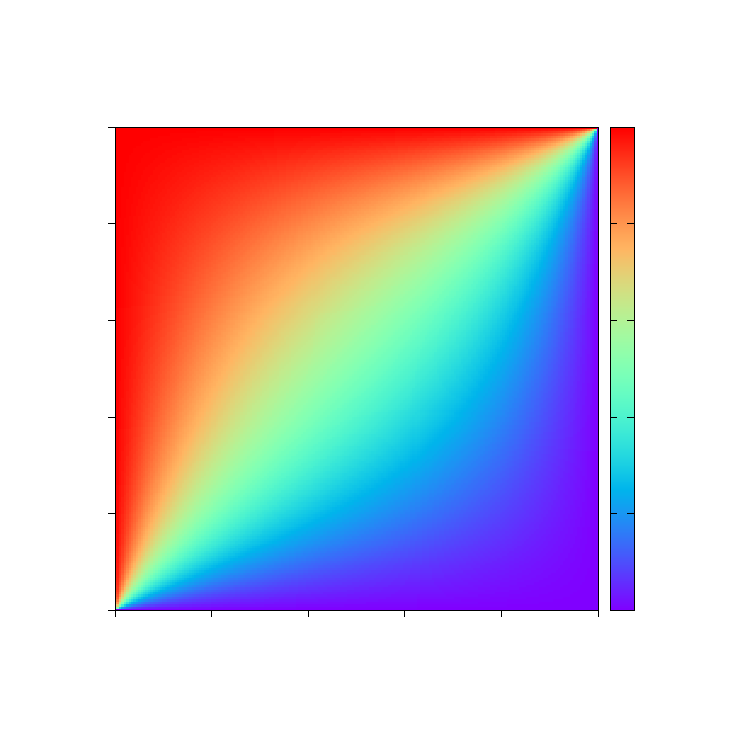
\includegraphics[width={340.10bp},height={340.10bp}]{diagonal_N200_Pe1.0e+00-inc}}%
    \gplfronttext
  \end{picture}%
\endgroup
\end{document}
}
%		% GNUPLOT: LaTeX picture with Postscript
\documentclass{minimal}
% Set font size
\makeatletter
\def\@ptsize{1}
\InputIfFileExists{size11.clo}{}{%
   \GenericError{(gnuplot) \space\space\space\@spaces}{%
      Gnuplot Error: File `size11.clo' not found! Could not set font size%
   }{See the gnuplot documentation for explanation.%
   }{For using a font size a file `size<fontsize>.clo' has to exist.
        Falling back ^^Jto default fontsize 10pt.}%
  \def\@ptsize{0}
  \input{size10.clo}%
}%
\makeatother
% Load packages
\usepackage{calc}
\usepackage{graphicx}
\usepackage{color}
\usepackage[cp1252]{inputenc}
\makeatletter
% Select an appropriate default driver (from TeXLive graphics.cfg)
\begingroup
  \chardef\x=0 %
  % check pdfTeX
  \@ifundefined{pdfoutput}{}{%
    \ifcase\pdfoutput
    \else
      \chardef\x=1 %
    \fi
  }%
  % check VTeX
  \@ifundefined{OpMode}{}{%
    \chardef\x=2 %
  }%
\expandafter\endgroup
\ifcase\x
  % default case
  \PassOptionsToPackage{dvips}{geometry}
\or
  % pdfTeX is running in pdf mode
  \PassOptionsToPackage{pdftex}{geometry}
\else
  % VTeX is running
  \PassOptionsToPackage{vtex}{geometry}
\fi
\makeatother
% Set papersize
\usepackage[papersize={340.10bp,340.10bp},text={340.10bp,340.10bp}]{geometry}
% No page numbers and no paragraph indentation
\pagestyle{empty}
\setlength{\parindent}{0bp}%
% Load configuration file
\InputIfFileExists{gnuplot.cfg}{%
  \typeout{Using configuration file gnuplot.cfg}%
}{%
 \typeout{No configuration file gnuplot.cfg found.}%
}%
%
\begin{document}
\begingroup
  % Encoding inside the plot.  In the header of your document, this encoding
  % should to defined, e.g., by using
  % \usepackage[cp1252,<other encodings>]{inputenc}
  \inputencoding{cp1252}%
  \makeatletter
  \providecommand\color[2][]{%
    \GenericError{(gnuplot) \space\space\space\@spaces}{%
      Package color not loaded in conjunction with
      terminal option `colourtext'%
    }{See the gnuplot documentation for explanation.%
    }{Either use 'blacktext' in gnuplot or load the package
      color.sty in LaTeX.}%
    \renewcommand\color[2][]{}%
  }%
  \providecommand\includegraphics[2][]{%
    \GenericError{(gnuplot) \space\space\space\@spaces}{%
      Package graphicx or graphics not loaded%
    }{See the gnuplot documentation for explanation.%
    }{The gnuplot epslatex terminal needs graphicx.sty or graphics.sty.}%
    \renewcommand\includegraphics[2][]{}%
  }%
  \providecommand\rotatebox[2]{#2}%
  \@ifundefined{ifGPcolor}{%
    \newif\ifGPcolor
    \GPcolortrue
  }{}%
  \@ifundefined{ifGPblacktext}{%
    \newif\ifGPblacktext
    \GPblacktextfalse
  }{}%
  % define a \g@addto@macro without @ in the name:
  \let\gplgaddtomacro\g@addto@macro
  % define empty templates for all commands taking text:
  \gdef\gplbacktext{}%
  \gdef\gplfronttext{}%
  \makeatother
  \ifGPblacktext
    % no textcolor at all
    \def\colorrgb#1{}%
    \def\colorgray#1{}%
  \else
    % gray or color?
    \ifGPcolor
      \def\colorrgb#1{\color[rgb]{#1}}%
      \def\colorgray#1{\color[gray]{#1}}%
      \expandafter\def\csname LTw\endcsname{\color{white}}%
      \expandafter\def\csname LTb\endcsname{\color{black}}%
      \expandafter\def\csname LTa\endcsname{\color{black}}%
      \expandafter\def\csname LT0\endcsname{\color[rgb]{1,0,0}}%
      \expandafter\def\csname LT1\endcsname{\color[rgb]{0,1,0}}%
      \expandafter\def\csname LT2\endcsname{\color[rgb]{0,0,1}}%
      \expandafter\def\csname LT3\endcsname{\color[rgb]{1,0,1}}%
      \expandafter\def\csname LT4\endcsname{\color[rgb]{0,1,1}}%
      \expandafter\def\csname LT5\endcsname{\color[rgb]{1,1,0}}%
      \expandafter\def\csname LT6\endcsname{\color[rgb]{0,0,0}}%
      \expandafter\def\csname LT7\endcsname{\color[rgb]{1,0.3,0}}%
      \expandafter\def\csname LT8\endcsname{\color[rgb]{0.5,0.5,0.5}}%
    \else
      % gray
      \def\colorrgb#1{\color{black}}%
      \def\colorgray#1{\color[gray]{#1}}%
      \expandafter\def\csname LTw\endcsname{\color{white}}%
      \expandafter\def\csname LTb\endcsname{\color{black}}%
      \expandafter\def\csname LTa\endcsname{\color{black}}%
      \expandafter\def\csname LT0\endcsname{\color{black}}%
      \expandafter\def\csname LT1\endcsname{\color{black}}%
      \expandafter\def\csname LT2\endcsname{\color{black}}%
      \expandafter\def\csname LT3\endcsname{\color{black}}%
      \expandafter\def\csname LT4\endcsname{\color{black}}%
      \expandafter\def\csname LT5\endcsname{\color{black}}%
      \expandafter\def\csname LT6\endcsname{\color{black}}%
      \expandafter\def\csname LT7\endcsname{\color{black}}%
      \expandafter\def\csname LT8\endcsname{\color{black}}%
    \fi
  \fi
    \setlength{\unitlength}{0.0500bp}%
    \ifx\gptboxheight\undefined%
      \newlength{\gptboxheight}%
      \newlength{\gptboxwidth}%
      \newsavebox{\gptboxtext}%
    \fi%
    \setlength{\fboxrule}{0.5pt}%
    \setlength{\fboxsep}{1pt}%
    \definecolor{tbcol}{rgb}{1,1,1}%
\begin{picture}(6802.00,6802.00)%
    \gplgaddtomacro\gplbacktext{%
      \csname LTb\endcsname%%
      \put(814,1105){\makebox(0,0)[r]{\strut{}0.0}}%
      \put(814,2032){\makebox(0,0)[r]{\strut{}0.2}}%
      \put(814,2959){\makebox(0,0)[r]{\strut{}0.4}}%
      \put(814,3886){\makebox(0,0)[r]{\strut{}0.6}}%
      \put(814,4813){\makebox(0,0)[r]{\strut{}0.8}}%
      \put(814,5740){\makebox(0,0)[r]{\strut{}1.0}}%
      \put(946,885){\makebox(0,0){\strut{}0.0}}%
      \put(1873,885){\makebox(0,0){\strut{}0.2}}%
      \put(2800,885){\makebox(0,0){\strut{}0.4}}%
      \put(3727,885){\makebox(0,0){\strut{}0.6}}%
      \put(4654,885){\makebox(0,0){\strut{}0.8}}%
      \put(5581,885){\makebox(0,0){\strut{}1.0}}%
    }%
    \gplgaddtomacro\gplfronttext{%
      \csname LTb\endcsname%%
      \put(209,3422){\rotatebox{-270}{\makebox(0,0){\strut{}$y \ (\mathrm{m})$}}}%
      \put(3263,555){\makebox(0,0){\strut{}$x \ (\mathrm{m})$}}%
      \csname LTb\endcsname%%
      \put(6060,1105){\makebox(0,0)[l]{\strut{}0.0}}%
      \put(6060,2032){\makebox(0,0)[l]{\strut{}0.2}}%
      \put(6060,2959){\makebox(0,0)[l]{\strut{}0.4}}%
      \put(6060,3886){\makebox(0,0)[l]{\strut{}0.6}}%
      \put(6060,4813){\makebox(0,0)[l]{\strut{}0.8}}%
      \put(6060,5740){\makebox(0,0)[l]{\strut{}1.0}}%
      \put(6522,3422){\rotatebox{-270}{\makebox(0,0){\strut{}$\phi$}}}%
      \put(3263,6070){\makebox(0,0){\strut{}\textbf{Diagonal case} $(\mathrm{Pe} = 1)$}}%
    }%
    \gplbacktext
    \put(0,0){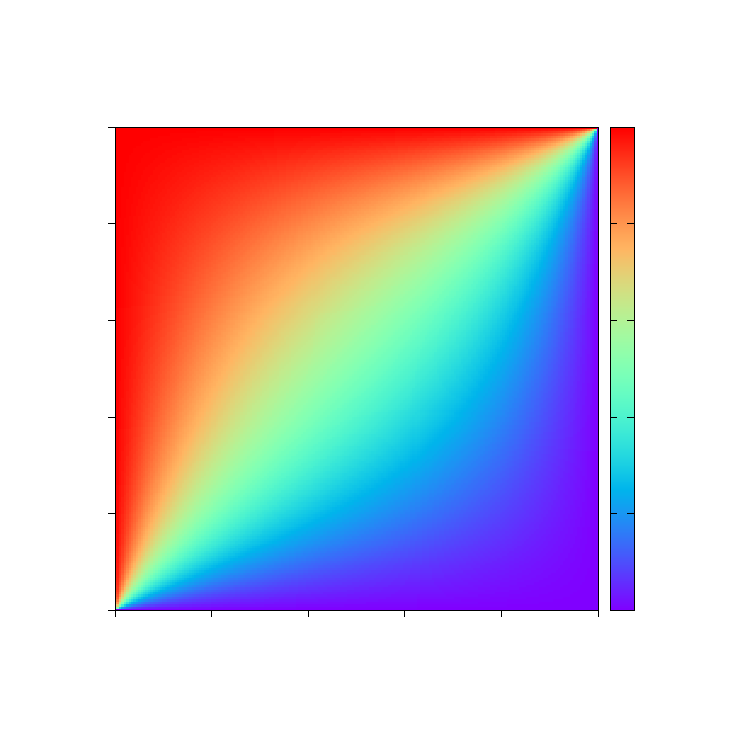
\includegraphics[width={340.10bp},height={340.10bp}]{diagonal_N200_Pe1.0e+00-inc}}%
    \gplfronttext
  \end{picture}%
\endgroup
\end{document}

%		\vspace{-0.75cm}
		\caption{Test}
		\label{fig:test1}
	\end{minipage}%
	\begin{minipage}{.5\textwidth}
		\centering
%		\vspace{-0.75cm}
		\fbox{% GNUPLOT: LaTeX picture with Postscript
\documentclass{minimal}
% Set font size
\makeatletter
\def\@ptsize{1}
\InputIfFileExists{size11.clo}{}{%
   \GenericError{(gnuplot) \space\space\space\@spaces}{%
      Gnuplot Error: File `size11.clo' not found! Could not set font size%
   }{See the gnuplot documentation for explanation.%
   }{For using a font size a file `size<fontsize>.clo' has to exist.
        Falling back ^^Jto default fontsize 10pt.}%
  \def\@ptsize{0}
  \input{size10.clo}%
}%
\makeatother
% Load packages
\usepackage{calc}
\usepackage{graphicx}
\usepackage{color}
\usepackage[cp1252]{inputenc}
\makeatletter
% Select an appropriate default driver (from TeXLive graphics.cfg)
\begingroup
  \chardef\x=0 %
  % check pdfTeX
  \@ifundefined{pdfoutput}{}{%
    \ifcase\pdfoutput
    \else
      \chardef\x=1 %
    \fi
  }%
  % check VTeX
  \@ifundefined{OpMode}{}{%
    \chardef\x=2 %
  }%
\expandafter\endgroup
\ifcase\x
  % default case
  \PassOptionsToPackage{dvips}{geometry}
\or
  % pdfTeX is running in pdf mode
  \PassOptionsToPackage{pdftex}{geometry}
\else
  % VTeX is running
  \PassOptionsToPackage{vtex}{geometry}
\fi
\makeatother
% Set papersize
\usepackage[papersize={340.10bp,340.10bp},text={340.10bp,340.10bp}]{geometry}
% No page numbers and no paragraph indentation
\pagestyle{empty}
\setlength{\parindent}{0bp}%
% Load configuration file
\InputIfFileExists{gnuplot.cfg}{%
  \typeout{Using configuration file gnuplot.cfg}%
}{%
 \typeout{No configuration file gnuplot.cfg found.}%
}%
%
\begin{document}
\begingroup
  % Encoding inside the plot.  In the header of your document, this encoding
  % should to defined, e.g., by using
  % \usepackage[cp1252,<other encodings>]{inputenc}
  \inputencoding{cp1252}%
  \makeatletter
  \providecommand\color[2][]{%
    \GenericError{(gnuplot) \space\space\space\@spaces}{%
      Package color not loaded in conjunction with
      terminal option `colourtext'%
    }{See the gnuplot documentation for explanation.%
    }{Either use 'blacktext' in gnuplot or load the package
      color.sty in LaTeX.}%
    \renewcommand\color[2][]{}%
  }%
  \providecommand\includegraphics[2][]{%
    \GenericError{(gnuplot) \space\space\space\@spaces}{%
      Package graphicx or graphics not loaded%
    }{See the gnuplot documentation for explanation.%
    }{The gnuplot epslatex terminal needs graphicx.sty or graphics.sty.}%
    \renewcommand\includegraphics[2][]{}%
  }%
  \providecommand\rotatebox[2]{#2}%
  \@ifundefined{ifGPcolor}{%
    \newif\ifGPcolor
    \GPcolortrue
  }{}%
  \@ifundefined{ifGPblacktext}{%
    \newif\ifGPblacktext
    \GPblacktextfalse
  }{}%
  % define a \g@addto@macro without @ in the name:
  \let\gplgaddtomacro\g@addto@macro
  % define empty templates for all commands taking text:
  \gdef\gplbacktext{}%
  \gdef\gplfronttext{}%
  \makeatother
  \ifGPblacktext
    % no textcolor at all
    \def\colorrgb#1{}%
    \def\colorgray#1{}%
  \else
    % gray or color?
    \ifGPcolor
      \def\colorrgb#1{\color[rgb]{#1}}%
      \def\colorgray#1{\color[gray]{#1}}%
      \expandafter\def\csname LTw\endcsname{\color{white}}%
      \expandafter\def\csname LTb\endcsname{\color{black}}%
      \expandafter\def\csname LTa\endcsname{\color{black}}%
      \expandafter\def\csname LT0\endcsname{\color[rgb]{1,0,0}}%
      \expandafter\def\csname LT1\endcsname{\color[rgb]{0,1,0}}%
      \expandafter\def\csname LT2\endcsname{\color[rgb]{0,0,1}}%
      \expandafter\def\csname LT3\endcsname{\color[rgb]{1,0,1}}%
      \expandafter\def\csname LT4\endcsname{\color[rgb]{0,1,1}}%
      \expandafter\def\csname LT5\endcsname{\color[rgb]{1,1,0}}%
      \expandafter\def\csname LT6\endcsname{\color[rgb]{0,0,0}}%
      \expandafter\def\csname LT7\endcsname{\color[rgb]{1,0.3,0}}%
      \expandafter\def\csname LT8\endcsname{\color[rgb]{0.5,0.5,0.5}}%
    \else
      % gray
      \def\colorrgb#1{\color{black}}%
      \def\colorgray#1{\color[gray]{#1}}%
      \expandafter\def\csname LTw\endcsname{\color{white}}%
      \expandafter\def\csname LTb\endcsname{\color{black}}%
      \expandafter\def\csname LTa\endcsname{\color{black}}%
      \expandafter\def\csname LT0\endcsname{\color{black}}%
      \expandafter\def\csname LT1\endcsname{\color{black}}%
      \expandafter\def\csname LT2\endcsname{\color{black}}%
      \expandafter\def\csname LT3\endcsname{\color{black}}%
      \expandafter\def\csname LT4\endcsname{\color{black}}%
      \expandafter\def\csname LT5\endcsname{\color{black}}%
      \expandafter\def\csname LT6\endcsname{\color{black}}%
      \expandafter\def\csname LT7\endcsname{\color{black}}%
      \expandafter\def\csname LT8\endcsname{\color{black}}%
    \fi
  \fi
    \setlength{\unitlength}{0.0500bp}%
    \ifx\gptboxheight\undefined%
      \newlength{\gptboxheight}%
      \newlength{\gptboxwidth}%
      \newsavebox{\gptboxtext}%
    \fi%
    \setlength{\fboxrule}{0.5pt}%
    \setlength{\fboxsep}{1pt}%
    \definecolor{tbcol}{rgb}{1,1,1}%
\begin{picture}(6802.00,6802.00)%
    \gplgaddtomacro\gplbacktext{%
      \csname LTb\endcsname%%
      \put(814,1105){\makebox(0,0)[r]{\strut{}0.0}}%
      \put(814,2032){\makebox(0,0)[r]{\strut{}0.2}}%
      \put(814,2959){\makebox(0,0)[r]{\strut{}0.4}}%
      \put(814,3886){\makebox(0,0)[r]{\strut{}0.6}}%
      \put(814,4813){\makebox(0,0)[r]{\strut{}0.8}}%
      \put(814,5740){\makebox(0,0)[r]{\strut{}1.0}}%
      \put(946,885){\makebox(0,0){\strut{}0.0}}%
      \put(1873,885){\makebox(0,0){\strut{}0.2}}%
      \put(2800,885){\makebox(0,0){\strut{}0.4}}%
      \put(3727,885){\makebox(0,0){\strut{}0.6}}%
      \put(4654,885){\makebox(0,0){\strut{}0.8}}%
      \put(5581,885){\makebox(0,0){\strut{}1.0}}%
    }%
    \gplgaddtomacro\gplfronttext{%
      \csname LTb\endcsname%%
      \put(209,3422){\rotatebox{-270}{\makebox(0,0){\strut{}$y \ (\mathrm{m})$}}}%
      \put(3263,555){\makebox(0,0){\strut{}$x \ (\mathrm{m})$}}%
      \csname LTb\endcsname%%
      \put(6060,1105){\makebox(0,0)[l]{\strut{}0.0}}%
      \put(6060,2032){\makebox(0,0)[l]{\strut{}0.2}}%
      \put(6060,2959){\makebox(0,0)[l]{\strut{}0.4}}%
      \put(6060,3886){\makebox(0,0)[l]{\strut{}0.6}}%
      \put(6060,4813){\makebox(0,0)[l]{\strut{}0.8}}%
      \put(6060,5740){\makebox(0,0)[l]{\strut{}1.0}}%
      \put(6522,3422){\rotatebox{-270}{\makebox(0,0){\strut{}$\phi$}}}%
      \put(3263,6070){\makebox(0,0){\strut{}\textbf{Diagonal case} $(\mathrm{Pe} = 1)$}}%
    }%
    \gplbacktext
    \put(0,0){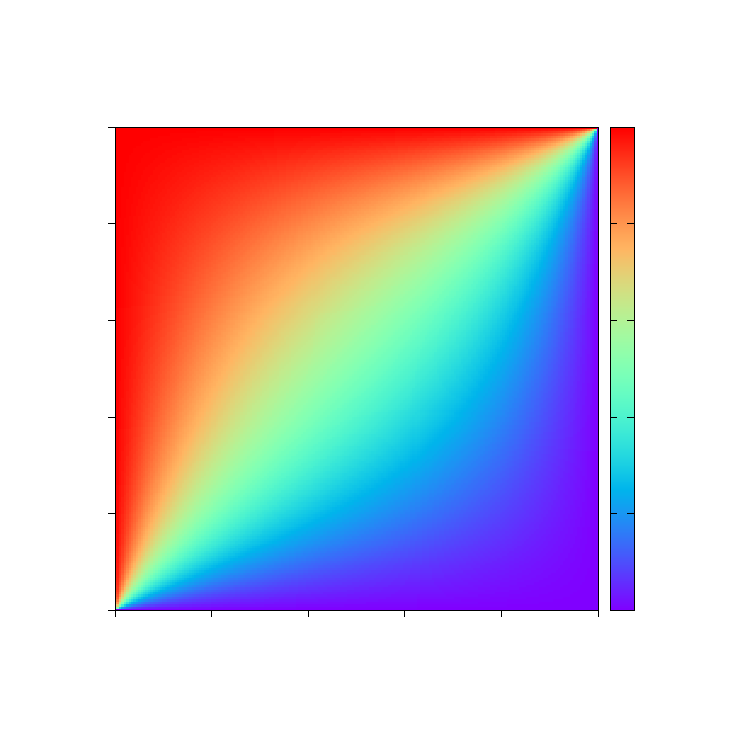
\includegraphics[width={340.10bp},height={340.10bp}]{diagonal_N200_Pe1.0e+00-inc}}%
    \gplfronttext
  \end{picture}%
\endgroup
\end{document}
}
%		% GNUPLOT: LaTeX picture with Postscript
\documentclass{minimal}
% Set font size
\makeatletter
\def\@ptsize{1}
\InputIfFileExists{size11.clo}{}{%
   \GenericError{(gnuplot) \space\space\space\@spaces}{%
      Gnuplot Error: File `size11.clo' not found! Could not set font size%
   }{See the gnuplot documentation for explanation.%
   }{For using a font size a file `size<fontsize>.clo' has to exist.
        Falling back ^^Jto default fontsize 10pt.}%
  \def\@ptsize{0}
  \input{size10.clo}%
}%
\makeatother
% Load packages
\usepackage{calc}
\usepackage{graphicx}
\usepackage{color}
\usepackage[cp1252]{inputenc}
\makeatletter
% Select an appropriate default driver (from TeXLive graphics.cfg)
\begingroup
  \chardef\x=0 %
  % check pdfTeX
  \@ifundefined{pdfoutput}{}{%
    \ifcase\pdfoutput
    \else
      \chardef\x=1 %
    \fi
  }%
  % check VTeX
  \@ifundefined{OpMode}{}{%
    \chardef\x=2 %
  }%
\expandafter\endgroup
\ifcase\x
  % default case
  \PassOptionsToPackage{dvips}{geometry}
\or
  % pdfTeX is running in pdf mode
  \PassOptionsToPackage{pdftex}{geometry}
\else
  % VTeX is running
  \PassOptionsToPackage{vtex}{geometry}
\fi
\makeatother
% Set papersize
\usepackage[papersize={340.10bp,340.10bp},text={340.10bp,340.10bp}]{geometry}
% No page numbers and no paragraph indentation
\pagestyle{empty}
\setlength{\parindent}{0bp}%
% Load configuration file
\InputIfFileExists{gnuplot.cfg}{%
  \typeout{Using configuration file gnuplot.cfg}%
}{%
 \typeout{No configuration file gnuplot.cfg found.}%
}%
%
\begin{document}
\begingroup
  % Encoding inside the plot.  In the header of your document, this encoding
  % should to defined, e.g., by using
  % \usepackage[cp1252,<other encodings>]{inputenc}
  \inputencoding{cp1252}%
  \makeatletter
  \providecommand\color[2][]{%
    \GenericError{(gnuplot) \space\space\space\@spaces}{%
      Package color not loaded in conjunction with
      terminal option `colourtext'%
    }{See the gnuplot documentation for explanation.%
    }{Either use 'blacktext' in gnuplot or load the package
      color.sty in LaTeX.}%
    \renewcommand\color[2][]{}%
  }%
  \providecommand\includegraphics[2][]{%
    \GenericError{(gnuplot) \space\space\space\@spaces}{%
      Package graphicx or graphics not loaded%
    }{See the gnuplot documentation for explanation.%
    }{The gnuplot epslatex terminal needs graphicx.sty or graphics.sty.}%
    \renewcommand\includegraphics[2][]{}%
  }%
  \providecommand\rotatebox[2]{#2}%
  \@ifundefined{ifGPcolor}{%
    \newif\ifGPcolor
    \GPcolortrue
  }{}%
  \@ifundefined{ifGPblacktext}{%
    \newif\ifGPblacktext
    \GPblacktextfalse
  }{}%
  % define a \g@addto@macro without @ in the name:
  \let\gplgaddtomacro\g@addto@macro
  % define empty templates for all commands taking text:
  \gdef\gplbacktext{}%
  \gdef\gplfronttext{}%
  \makeatother
  \ifGPblacktext
    % no textcolor at all
    \def\colorrgb#1{}%
    \def\colorgray#1{}%
  \else
    % gray or color?
    \ifGPcolor
      \def\colorrgb#1{\color[rgb]{#1}}%
      \def\colorgray#1{\color[gray]{#1}}%
      \expandafter\def\csname LTw\endcsname{\color{white}}%
      \expandafter\def\csname LTb\endcsname{\color{black}}%
      \expandafter\def\csname LTa\endcsname{\color{black}}%
      \expandafter\def\csname LT0\endcsname{\color[rgb]{1,0,0}}%
      \expandafter\def\csname LT1\endcsname{\color[rgb]{0,1,0}}%
      \expandafter\def\csname LT2\endcsname{\color[rgb]{0,0,1}}%
      \expandafter\def\csname LT3\endcsname{\color[rgb]{1,0,1}}%
      \expandafter\def\csname LT4\endcsname{\color[rgb]{0,1,1}}%
      \expandafter\def\csname LT5\endcsname{\color[rgb]{1,1,0}}%
      \expandafter\def\csname LT6\endcsname{\color[rgb]{0,0,0}}%
      \expandafter\def\csname LT7\endcsname{\color[rgb]{1,0.3,0}}%
      \expandafter\def\csname LT8\endcsname{\color[rgb]{0.5,0.5,0.5}}%
    \else
      % gray
      \def\colorrgb#1{\color{black}}%
      \def\colorgray#1{\color[gray]{#1}}%
      \expandafter\def\csname LTw\endcsname{\color{white}}%
      \expandafter\def\csname LTb\endcsname{\color{black}}%
      \expandafter\def\csname LTa\endcsname{\color{black}}%
      \expandafter\def\csname LT0\endcsname{\color{black}}%
      \expandafter\def\csname LT1\endcsname{\color{black}}%
      \expandafter\def\csname LT2\endcsname{\color{black}}%
      \expandafter\def\csname LT3\endcsname{\color{black}}%
      \expandafter\def\csname LT4\endcsname{\color{black}}%
      \expandafter\def\csname LT5\endcsname{\color{black}}%
      \expandafter\def\csname LT6\endcsname{\color{black}}%
      \expandafter\def\csname LT7\endcsname{\color{black}}%
      \expandafter\def\csname LT8\endcsname{\color{black}}%
    \fi
  \fi
    \setlength{\unitlength}{0.0500bp}%
    \ifx\gptboxheight\undefined%
      \newlength{\gptboxheight}%
      \newlength{\gptboxwidth}%
      \newsavebox{\gptboxtext}%
    \fi%
    \setlength{\fboxrule}{0.5pt}%
    \setlength{\fboxsep}{1pt}%
    \definecolor{tbcol}{rgb}{1,1,1}%
\begin{picture}(6802.00,6802.00)%
    \gplgaddtomacro\gplbacktext{%
      \csname LTb\endcsname%%
      \put(814,1105){\makebox(0,0)[r]{\strut{}0.0}}%
      \put(814,2032){\makebox(0,0)[r]{\strut{}0.2}}%
      \put(814,2959){\makebox(0,0)[r]{\strut{}0.4}}%
      \put(814,3886){\makebox(0,0)[r]{\strut{}0.6}}%
      \put(814,4813){\makebox(0,0)[r]{\strut{}0.8}}%
      \put(814,5740){\makebox(0,0)[r]{\strut{}1.0}}%
      \put(946,885){\makebox(0,0){\strut{}0.0}}%
      \put(1873,885){\makebox(0,0){\strut{}0.2}}%
      \put(2800,885){\makebox(0,0){\strut{}0.4}}%
      \put(3727,885){\makebox(0,0){\strut{}0.6}}%
      \put(4654,885){\makebox(0,0){\strut{}0.8}}%
      \put(5581,885){\makebox(0,0){\strut{}1.0}}%
    }%
    \gplgaddtomacro\gplfronttext{%
      \csname LTb\endcsname%%
      \put(209,3422){\rotatebox{-270}{\makebox(0,0){\strut{}$y \ (\mathrm{m})$}}}%
      \put(3263,555){\makebox(0,0){\strut{}$x \ (\mathrm{m})$}}%
      \csname LTb\endcsname%%
      \put(6060,1105){\makebox(0,0)[l]{\strut{}0.0}}%
      \put(6060,2032){\makebox(0,0)[l]{\strut{}0.2}}%
      \put(6060,2959){\makebox(0,0)[l]{\strut{}0.4}}%
      \put(6060,3886){\makebox(0,0)[l]{\strut{}0.6}}%
      \put(6060,4813){\makebox(0,0)[l]{\strut{}0.8}}%
      \put(6060,5740){\makebox(0,0)[l]{\strut{}1.0}}%
      \put(6522,3422){\rotatebox{-270}{\makebox(0,0){\strut{}$\phi$}}}%
      \put(3263,6070){\makebox(0,0){\strut{}\textbf{Diagonal case} $(\mathrm{Pe} = 1)$}}%
    }%
    \gplbacktext
    \put(0,0){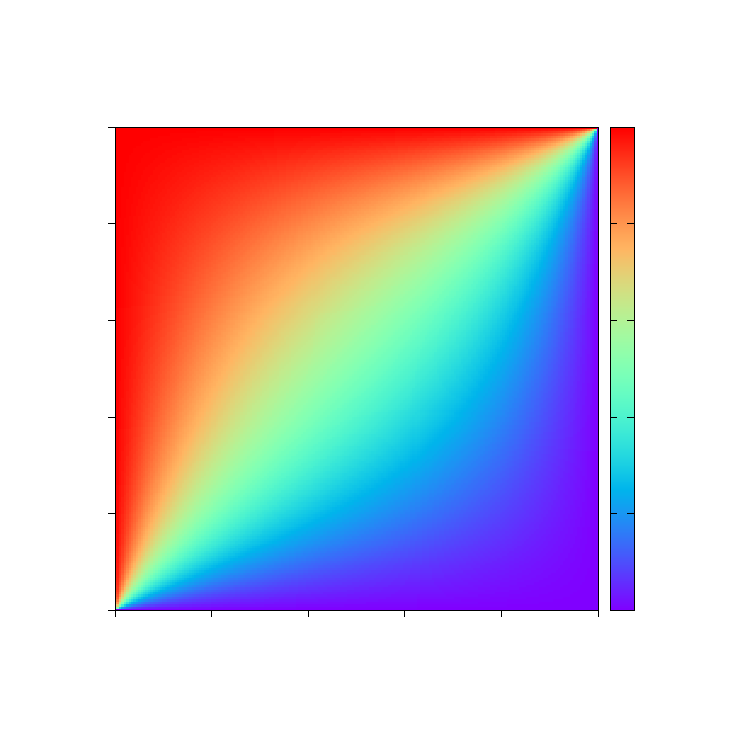
\includegraphics[width={340.10bp},height={340.10bp}]{diagonal_N200_Pe1.0e+00-inc}}%
    \gplfronttext
  \end{picture}%
\endgroup
\end{document}

%		\vspace{-0.75cm}
		\caption{Test}
		\label{fig:test2}
	\end{minipage}
\end{figure}


\clearpage	
\section{Smith--Hutton case} \label{sec:smith_hutton_case}


\subsection{Statement}

This section deals with the steady state version of the problem proposed by
Smith and Hutton (1982) described in \cite{smith1982numerical}. The problem
takes place in the domain $\Omega = (-L,L) \times (0,L) \subset \real^2$ where
$L > 0$ is a constant length. Both density and diffusion coefficient are assumed
to be constant and known values. In $\Omega$ the steady state version of the
general convection--diffusion equation with no source term is considered, that
is,
\begin{equation*}
	\frac{\rho}{\Gamma} \vb{v} \vdot \grad{\phi} = \Delta{\phi}
\end{equation*}
On the boundary of $\Omega$ the following conditions are prescribed:
\begin{itemize}[topsep=0pt]
	\item $\phi = 1 + \tanh(10(2x+1))$ on $C_1 = [-L,0] \times \{ 0 \}$ (inlet
	flow).
	\item $\phi = 1 - \tanh(10)$ on $C_2 = \left( \{ -L \} \times (0,L) \right)
	\cup \left( [-L,L] \times \{ L \} \right) \cup \left( \{ L \} \times [0,L)
	\right)$.
	\item $\phi_y = 0$ on $C_3 = (0,L) \times \{ 0
	\}$ (outlet flow).
\end{itemize}
Notice that the curves $C_1, C_2, C_3$ give a partition of $\partial \Omega$. To
encode the first two boundary conditions in a compact manner, we define the
function $g \colon C_1 \cup C_2 \rightarrow \real$ by
\begin{equation*}
	g(x,y) = 
	\left\{
	\begin{aligned}
		&1 + \tanh(10(2x + 1)) 	& &\text{if } (x,y) \in C_1 \\
		&1 - \tanh(10) 			& &\text{if } (x,y) \in C_2
	\end{aligned}
	\right.
\end{equation*}
The velocity field is given by $u = 2 y (1 - x^2)$ and $v = -2 x (1 - y^2)$. The
resulting Cauchy problem is given by \eqref{eq:smith_hutton_cauchy_problem} and
summarized in figure \ref{fig:smith_hutton_cauchy_problem}.
\begin{equation} \label{eq:smith_hutton_cauchy_problem} 
	\left\{
	\begin{aligned}
		\Delta \phi - \frac{\rho}{\Gamma} \vb{v} \vdot \grad{\phi} &= 0 &
		&\text{in } \Omega \\
		\phi &= g & 
		&\text{on } C_1 \cup C_2 \\
		\phi_y &= 0 & 
		&\text{on } C_3
	\end{aligned}
	\right.
\end{equation}

\begin{figure}[h]
	\centering
	\begin{tikzpicture}
		% Lenghts
		\def\alength{5} \def\L{4.5} \def\mlength{0.1}
		% Domain
		\fill[cyan!70!white] (-\L,0) rectangle (\L, \L); \draw[thick, thick]
		(-\L,0) rectangle (\L, \L);
		% Axis
		\draw[-stealth] (-\alength,0) -- (\alength,0) node[above]{$x$};
		\draw[-stealth] (0,-0.5) -- (0,\alength) node[right]{$y$}; \draw[black,
		thick] (\L,0) node[left, yshift=3mm]{$L$} -- ++(0,-\mlength);
		\draw[black, thick] (-\L,0) node[right, yshift=3mm]{$-L$} --
		++(0,-\mlength);
		% Right boundary condition
		\node[inner sep=0pt] at (\L,{0.5*\L}) (rb) {}; \node[] at
		({\L+2},{0.5*\L+1}) (rbc) {$\phi = 1 - \tanh(10)$}; \path[-latex] (rbc)
		edge[bend left] node [left] {} (rb);
		% Top boundary condition
		\node[inner sep=0pt] at ({0.1*\L},\L) (tb) {}; \node[] at
		({0.1*\L+2},{\L+1}) (tbc) {$\phi = 1 - \tanh(10)$}; \path[-latex] (tbc)
		edge[bend right] node [left] {} (tb);
		% Left boundary condition
		\node[inner sep=0pt] at (-\L,{0.5*\L}) (lb) {}; \node[] at
		(-\L-2,{0.5*\L-1}) (lbc) {$\phi = 1 - \tanh(10)$}; \path[-latex] (lbc)
		edge[bend left] node [left] {} (lb);
		% Right bottom boundary condition
		\node[inner sep=0pt] at ({0.5*\L},0) (bb) {}; \node[] at
		({0.5*\L-1},-0.5) (bbc) {$\partial_y \phi = 0$}; \path[-latex] (bbc)
		edge[bend right] node [left] {} (bb);
		% Left bottom boundary condition
		\node[inner sep=0pt] at ({-0.1*\L},0) (lbb) {}; \node[] at ({-\L},-0.5)
		(lbbc) {$\phi = 1 + \tanh(10(2x+1))$}; \path[-latex] (lbbc) edge[bend
		right] node [left] {} (lbb);
		% PDE outer sep=0pt, greenNode, yshift=3mm, fill=white
		\node[fill=cyan!70!white] at (0,{0.5*\L}) {$\Delta \phi -
		\frac{\rho}{\Gamma} \vb{v} \vdot \grad{\phi} = 0$};
		% Inlet and outlet
		\node[] at ({-0.5*\L},0.3) {Inlet}; \node[] at ({0.5*\L},0.3) {Outlet};
	\end{tikzpicture}
	\caption{Cauchy problem for the diagonal flow case.}
	\label{fig:smith_hutton_cauchy_problem}
\end{figure}







\subsection{Velocity field}

The velocity field for the Smith-Hutton case is given by $\vb{v} = 2 y (1 - x^2)
\vb{i} - 2 x (1 - y^2) \vb{j}$. It verifies the incompressibility condition
since it is divergence--free, \ie $\div{\vb{v}} = 0$. The only points where
$\vb{v}$ vanishes are $(0,0)$ and $(\pm 1, \pm 1)$. In the case of $L < 1$, only
$(0,0)$ belongs to $\overline{\Omega}$. Otherwise, $(0,0)$, $(-1,1)$ and $(1,1)$
the first three points belong to $\overline{\Omega}$. 

Recall that the
stream function is a mapping $\psi \colon U \subset \real^2 \to \real$, where
$U$ is some open subset of $\real^2$ containing $\Omega$, such that
\begin{equation} \label{eq:stream_function_definition}
	u = \pdv{\psi}{y}, \quad
	v = -\pdv{\psi}{x}
\end{equation}
By choosing $u$ and $v$ to be the components of the velocity field $\vb{v}$ and
integrating, one finds the function $\psi(x,y) = x^2 + y^2 (1 - x^2) + C$ where
$C \in \real$ is a constant. Since the constant vanishes when differentiating,
we may choose $C = -1$ so that we obtain the more nice looking
\begin{equation}
	\psi(x,y) = -(1 - x^2)(1 - y^2)
\end{equation}

\colorbox{red}{In this and in the forthcoming sections we shall assume $L = 1$. }

In order to find the analytical solution to problem
\eqref{eq:smith_hutton_cauchy_problem} when $\Gamma = 0$, it will be useful to
know how the streamlines are. Recall that the streamlines are defined as the
curves tangent to the vector field $\vb{v}$ at each point. If $\alpha \colon I
\subset \real \to \Omega$, $s \mapsto \alpha(s) = (x(s), y(s))$ is the
parametrization of a curve in $\Omega$, then it is a streamline provided it
satisifes the following system of ODEs:
\begin{equation} \label{eq:velocity_smith_hutton_odes}
	\left\{
	\begin{aligned}
		x' &= 2 y (1 - x^2) \\
		y' &= - 2 x (1 - y^2)
	\end{aligned}
	\right.
\end{equation}
Equivalently, the streamlines are the curves with normal vector $\grad{\psi}$
at every point. In order to find the streamlines, we can specify an initial
condition and then pose an initial value problem. Consider the mapping $f \colon
\real^2 \longrightarrow \real^2$ defined by
\begin{equation}
	f(x,y) = 
	\begin{pmatrix}
		u(x,y) \\ v(x,y)
	\end{pmatrix} =
	\begin{pmatrix}
		2 y (1 - x^2) \\ - 2 x (1 - y^2)
	\end{pmatrix}
\end{equation}
Then the initial value problem for a streamline with initial condition $(x_0,y_0) \in \overline{\Omega}$ is
\begin{equation} \label{eq:vel_smith_hutton_ivp}
	\left\{
		\begin{aligned}
			\alpha' &= f(\alpha(s)) \\
			\alpha(0) &= (x_0, y_0)
		\end{aligned}
	\right.
\end{equation}

\begin{prop}
	The solution to the initial value problem \eqref{eq:vel_smith_hutton_ivp}
	exists and is unique for every $(x_0, y_0) \in \overline{\Omega}$.
\end{prop}
\begin{proof}
	Let $U = B(0,2L)$, thus $\overline{\Omega} \subset U$. Since both $u$ and
	$v$ are $\mathcal{C}^\infty(\real^2)$ functions, $f$ is
	$\mathcal{C}^\infty(\real^2)$. The restriction of $f$ to $\overline{U}$ is,
	in particular, a $\mathcal{C}^1(\overline{U})$ mapping. By theorem
	\ref{teo:c1_function_implies_lipschitz}, $f$ is Lipschitz on $\overline{U}$.
	Now by the Picard--Lindelöf theorem (Theorem \ref{teo:picard_lindelof}) we
	deduce the existence and uniqueness of solution to
	\eqref{eq:vel_smith_hutton_ivp}.
\end{proof}

Finding the explicit solution to \eqref{eq:vel_smith_hutton_ivp} might be
difficult as the system is non--linear. Nonetheless we can solve it numerically
so as to find the appearance of the streamlines. This is precisely what has been
done to produce figure \eqref{fig:smith_hutton_N201_streamlines}. The RK4
algorithm was applied to the IVP \eqref{eq:vel_smith_hutton_ivp} for $L = 1 \
\meter$ and initial conditions $x_0 = 0.10, \ 0.20, \ 0.30, \ 0.40, \ 0.50, \
0.60, \ 0.70, \ 0.80, \ 0.90, \ 0.99 \ \meter$ and $y_0 = 0$.

\begin{figure}[ht]
	\centering
	%	\fbox{% GNUPLOT: LaTeX picture with Postscript
\begingroup
  % Encoding inside the plot.  In the header of your document, this encoding
  % should to defined, e.g., by using
  % \usepackage[cp1252,<other encodings>]{inputenc}
  \inputencoding{cp1252}%
  \makeatletter
  \providecommand\color[2][]{%
    \GenericError{(gnuplot) \space\space\space\@spaces}{%
      Package color not loaded in conjunction with
      terminal option `colourtext'%
    }{See the gnuplot documentation for explanation.%
    }{Either use 'blacktext' in gnuplot or load the package
      color.sty in LaTeX.}%
    \renewcommand\color[2][]{}%
  }%
  \providecommand\includegraphics[2][]{%
    \GenericError{(gnuplot) \space\space\space\@spaces}{%
      Package graphicx or graphics not loaded%
    }{See the gnuplot documentation for explanation.%
    }{The gnuplot epslatex terminal needs graphicx.sty or graphics.sty.}%
    \renewcommand\includegraphics[2][]{}%
  }%
  \providecommand\rotatebox[2]{#2}%
  \@ifundefined{ifGPcolor}{%
    \newif\ifGPcolor
    \GPcolortrue
  }{}%
  \@ifundefined{ifGPblacktext}{%
    \newif\ifGPblacktext
    \GPblacktextfalse
  }{}%
  % define a \g@addto@macro without @ in the name:
  \let\gplgaddtomacro\g@addto@macro
  % define empty templates for all commands taking text:
  \gdef\gplbacktext{}%
  \gdef\gplfronttext{}%
  \makeatother
  \ifGPblacktext
    % no textcolor at all
    \def\colorrgb#1{}%
    \def\colorgray#1{}%
  \else
    % gray or color?
    \ifGPcolor
      \def\colorrgb#1{\color[rgb]{#1}}%
      \def\colorgray#1{\color[gray]{#1}}%
      \expandafter\def\csname LTw\endcsname{\color{white}}%
      \expandafter\def\csname LTb\endcsname{\color{black}}%
      \expandafter\def\csname LTa\endcsname{\color{black}}%
      \expandafter\def\csname LT0\endcsname{\color[rgb]{1,0,0}}%
      \expandafter\def\csname LT1\endcsname{\color[rgb]{0,1,0}}%
      \expandafter\def\csname LT2\endcsname{\color[rgb]{0,0,1}}%
      \expandafter\def\csname LT3\endcsname{\color[rgb]{1,0,1}}%
      \expandafter\def\csname LT4\endcsname{\color[rgb]{0,1,1}}%
      \expandafter\def\csname LT5\endcsname{\color[rgb]{1,1,0}}%
      \expandafter\def\csname LT6\endcsname{\color[rgb]{0,0,0}}%
      \expandafter\def\csname LT7\endcsname{\color[rgb]{1,0.3,0}}%
      \expandafter\def\csname LT8\endcsname{\color[rgb]{0.5,0.5,0.5}}%
    \else
      % gray
      \def\colorrgb#1{\color{black}}%
      \def\colorgray#1{\color[gray]{#1}}%
      \expandafter\def\csname LTw\endcsname{\color{white}}%
      \expandafter\def\csname LTb\endcsname{\color{black}}%
      \expandafter\def\csname LTa\endcsname{\color{black}}%
      \expandafter\def\csname LT0\endcsname{\color{black}}%
      \expandafter\def\csname LT1\endcsname{\color{black}}%
      \expandafter\def\csname LT2\endcsname{\color{black}}%
      \expandafter\def\csname LT3\endcsname{\color{black}}%
      \expandafter\def\csname LT4\endcsname{\color{black}}%
      \expandafter\def\csname LT5\endcsname{\color{black}}%
      \expandafter\def\csname LT6\endcsname{\color{black}}%
      \expandafter\def\csname LT7\endcsname{\color{black}}%
      \expandafter\def\csname LT8\endcsname{\color{black}}%
    \fi
  \fi
    \setlength{\unitlength}{0.0500bp}%
    \ifx\gptboxheight\undefined%
      \newlength{\gptboxheight}%
      \newlength{\gptboxwidth}%
      \newsavebox{\gptboxtext}%
    \fi%
    \setlength{\fboxrule}{0.5pt}%
    \setlength{\fboxsep}{1pt}%
    \definecolor{tbcol}{rgb}{1,1,1}%
\begin{picture}(7370.00,3968.00)%
    \gplgaddtomacro\gplbacktext{%
      \csname LTb\endcsname%%
      \put(814,719){\makebox(0,0)[r]{\strut{}0.0}}%
      \put(814,1234){\makebox(0,0)[r]{\strut{}0.2}}%
      \put(814,1748){\makebox(0,0)[r]{\strut{}0.4}}%
      \put(814,2263){\makebox(0,0)[r]{\strut{}0.6}}%
      \put(814,2777){\makebox(0,0)[r]{\strut{}0.8}}%
      \put(814,3292){\makebox(0,0)[r]{\strut{}1.0}}%
      \put(946,499){\makebox(0,0){\strut{}-1.0}}%
      \put(2233,499){\makebox(0,0){\strut{}-0.5}}%
      \put(3520,499){\makebox(0,0){\strut{}0.0}}%
      \put(4806,499){\makebox(0,0){\strut{}0.5}}%
      \put(6093,499){\makebox(0,0){\strut{}1.0}}%
    }%
    \gplgaddtomacro\gplfronttext{%
      \csname LTb\endcsname%%
      \put(209,2005){\rotatebox{-270}{\makebox(0,0){\strut{}$y \ (\mathrm{m})$}}}%
      \put(3519,169){\makebox(0,0){\strut{}$x \ (\mathrm{m})$}}%
      \csname LTb\endcsname%%
      \put(6611,719){\makebox(0,0)[l]{\strut{}0.0}}%
      \put(6611,1362){\makebox(0,0)[l]{\strut{}0.5}}%
      \put(6611,2005){\makebox(0,0)[l]{\strut{}1.0}}%
      \put(6611,2648){\makebox(0,0)[l]{\strut{}1.5}}%
      \put(6611,3292){\makebox(0,0)[l]{\strut{}2.0}}%
      \put(7073,2005){\rotatebox{-270}{\makebox(0,0){\strut{}$\phi$}}}%
      \put(3519,3622){\makebox(0,0){\strut{}\textbf{Smith--Hutton case} $(\mathrm{Pe} = 10^{2})$}}%
    }%
    \gplbacktext
    \put(0,0){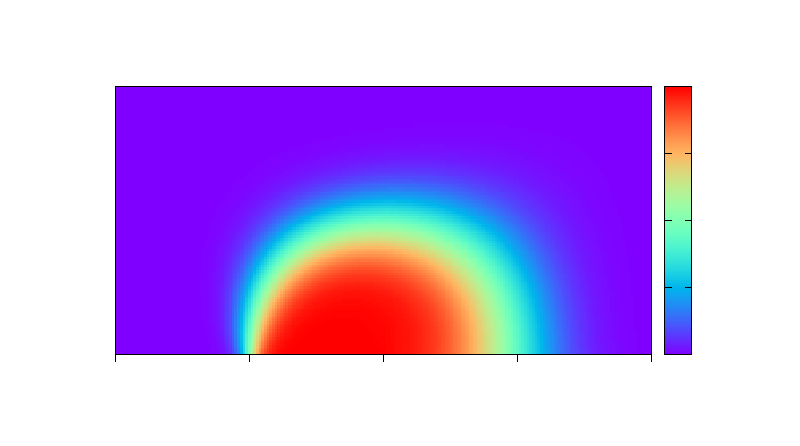
\includegraphics[width={368.50bp},height={198.40bp}]{figures/case_smith_hutton/smith_hutton_N201_Pe1.0e+02}}%
    \gplfronttext
  \end{picture}%
\endgroup
}
	% GNUPLOT: LaTeX picture with Postscript
\begingroup
  % Encoding inside the plot.  In the header of your document, this encoding
  % should to defined, e.g., by using
  % \usepackage[cp1252,<other encodings>]{inputenc}
  \inputencoding{cp1252}%
  \makeatletter
  \providecommand\color[2][]{%
    \GenericError{(gnuplot) \space\space\space\@spaces}{%
      Package color not loaded in conjunction with
      terminal option `colourtext'%
    }{See the gnuplot documentation for explanation.%
    }{Either use 'blacktext' in gnuplot or load the package
      color.sty in LaTeX.}%
    \renewcommand\color[2][]{}%
  }%
  \providecommand\includegraphics[2][]{%
    \GenericError{(gnuplot) \space\space\space\@spaces}{%
      Package graphicx or graphics not loaded%
    }{See the gnuplot documentation for explanation.%
    }{The gnuplot epslatex terminal needs graphicx.sty or graphics.sty.}%
    \renewcommand\includegraphics[2][]{}%
  }%
  \providecommand\rotatebox[2]{#2}%
  \@ifundefined{ifGPcolor}{%
    \newif\ifGPcolor
    \GPcolortrue
  }{}%
  \@ifundefined{ifGPblacktext}{%
    \newif\ifGPblacktext
    \GPblacktextfalse
  }{}%
  % define a \g@addto@macro without @ in the name:
  \let\gplgaddtomacro\g@addto@macro
  % define empty templates for all commands taking text:
  \gdef\gplbacktext{}%
  \gdef\gplfronttext{}%
  \makeatother
  \ifGPblacktext
    % no textcolor at all
    \def\colorrgb#1{}%
    \def\colorgray#1{}%
  \else
    % gray or color?
    \ifGPcolor
      \def\colorrgb#1{\color[rgb]{#1}}%
      \def\colorgray#1{\color[gray]{#1}}%
      \expandafter\def\csname LTw\endcsname{\color{white}}%
      \expandafter\def\csname LTb\endcsname{\color{black}}%
      \expandafter\def\csname LTa\endcsname{\color{black}}%
      \expandafter\def\csname LT0\endcsname{\color[rgb]{1,0,0}}%
      \expandafter\def\csname LT1\endcsname{\color[rgb]{0,1,0}}%
      \expandafter\def\csname LT2\endcsname{\color[rgb]{0,0,1}}%
      \expandafter\def\csname LT3\endcsname{\color[rgb]{1,0,1}}%
      \expandafter\def\csname LT4\endcsname{\color[rgb]{0,1,1}}%
      \expandafter\def\csname LT5\endcsname{\color[rgb]{1,1,0}}%
      \expandafter\def\csname LT6\endcsname{\color[rgb]{0,0,0}}%
      \expandafter\def\csname LT7\endcsname{\color[rgb]{1,0.3,0}}%
      \expandafter\def\csname LT8\endcsname{\color[rgb]{0.5,0.5,0.5}}%
    \else
      % gray
      \def\colorrgb#1{\color{black}}%
      \def\colorgray#1{\color[gray]{#1}}%
      \expandafter\def\csname LTw\endcsname{\color{white}}%
      \expandafter\def\csname LTb\endcsname{\color{black}}%
      \expandafter\def\csname LTa\endcsname{\color{black}}%
      \expandafter\def\csname LT0\endcsname{\color{black}}%
      \expandafter\def\csname LT1\endcsname{\color{black}}%
      \expandafter\def\csname LT2\endcsname{\color{black}}%
      \expandafter\def\csname LT3\endcsname{\color{black}}%
      \expandafter\def\csname LT4\endcsname{\color{black}}%
      \expandafter\def\csname LT5\endcsname{\color{black}}%
      \expandafter\def\csname LT6\endcsname{\color{black}}%
      \expandafter\def\csname LT7\endcsname{\color{black}}%
      \expandafter\def\csname LT8\endcsname{\color{black}}%
    \fi
  \fi
    \setlength{\unitlength}{0.0500bp}%
    \ifx\gptboxheight\undefined%
      \newlength{\gptboxheight}%
      \newlength{\gptboxwidth}%
      \newsavebox{\gptboxtext}%
    \fi%
    \setlength{\fboxrule}{0.5pt}%
    \setlength{\fboxsep}{1pt}%
    \definecolor{tbcol}{rgb}{1,1,1}%
\begin{picture}(7370.00,3968.00)%
    \gplgaddtomacro\gplbacktext{%
      \csname LTb\endcsname%%
      \put(814,733){\makebox(0,0)[r]{\strut{}$0$}}%
      \put(814,1242){\makebox(0,0)[r]{\strut{}$0.2$}}%
      \put(814,1751){\makebox(0,0)[r]{\strut{}$0.4$}}%
      \put(814,2260){\makebox(0,0)[r]{\strut{}$0.6$}}%
      \put(814,2769){\makebox(0,0)[r]{\strut{}$0.8$}}%
      \put(814,3278){\makebox(0,0)[r]{\strut{}$1$}}%
      \put(1009,513){\makebox(0,0){\strut{}-1.0}}%
      \put(2282,513){\makebox(0,0){\strut{}-0.5}}%
      \put(3554,513){\makebox(0,0){\strut{}0.0}}%
      \put(4827,513){\makebox(0,0){\strut{}0.5}}%
      \put(6099,513){\makebox(0,0){\strut{}1.0}}%
    }%
    \gplgaddtomacro\gplfronttext{%
      \csname LTb\endcsname%%
      \put(209,2005){\rotatebox{-270}{\makebox(0,0){\strut{}$y \ (\mathrm{m})$}}}%
      \put(3554,183){\makebox(0,0){\strut{}$x \ (\mathrm{m})$}}%
      \csname LTb\endcsname%%
      \put(6612,733){\makebox(0,0)[l]{\strut{}0.0}}%
      \put(6612,1369){\makebox(0,0)[l]{\strut{}0.5}}%
      \put(6612,2005){\makebox(0,0)[l]{\strut{}1.0}}%
      \put(6612,2641){\makebox(0,0)[l]{\strut{}1.5}}%
      \put(6612,3278){\makebox(0,0)[l]{\strut{}2.0}}%
      \put(7074,2005){\rotatebox{-270}{\makebox(0,0){\strut{}$\norm{\vb{v}} \ (\mathrm{m} / \mathrm{s})$}}}%
      \put(3554,3608){\makebox(0,0){\strut{}\textbf{Smith--Hutton case -- Velocity field}}}%
    }%
    \gplbacktext
    \put(0,0){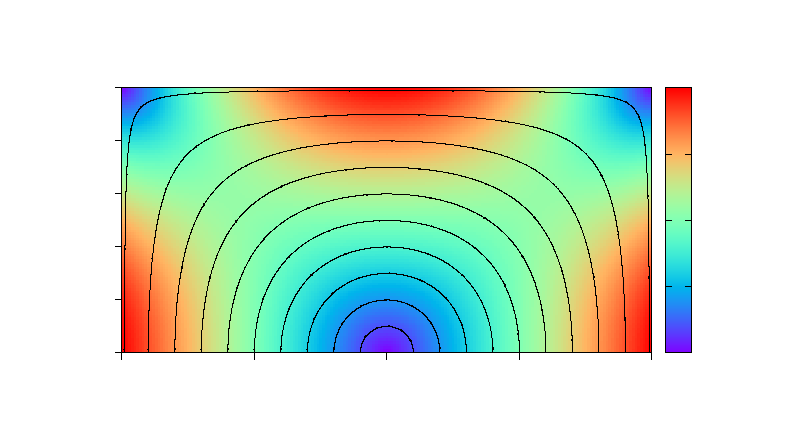
\includegraphics[width={368.50bp},height={198.40bp}]{figures/case_smith_hutton/smith_hutton_N201_streamlines}}%
    \gplfronttext
  \end{picture}%
\endgroup

	\captionsetup{width=0.75\textwidth}
	\caption{Norm of the Smith--Hutton velocity field and streamlines for $x_0 =
	0.10, \ 0.20, \ 0.30, \ 0.40, \ 0.50, \ 0.60, \ 0.70, \ 0.80, \ 0.90$ and
	$0.99 \ \meter$. The vectors tangent to the streamlines are normalized and
	then scaled down by a factor of $\sqrt{2}/50$.}
	\label{fig:smith_hutton_N201_streamlines}
\end{figure}

\subsection{Analytical solution}

As we have previously seen, Péclet's number is defined as
\begin{equation}
	\peclet = 
	\frac{\text{convection transport rate}}{\text{diffusion transport rate}} = 
	\frac{\rho v_0 L}{\Gamma}
\end{equation}
Note that the factor $\beta$ in the PDE from problem
\eqref{eq:diagonal_case_cauchy_problem} is a constant determined by the
geometry, whereas Peclet's number depends on the fluid and on the velocity
field. Since no more factors intervene on the PDE, this tells us that the
behaviour of the solution will depend greatly on Peclet's number. 

\subsubsection{Classical solution for \texorpdfstring{$\peclet =
\infty$}{infinite Péclet's number}}

Whenever $\peclet \to +\infty$, it implies $\Gamma \to 0^+$ since infinite
values for the density, velocity or characteristic length make no physical
sense. Therefore the difussion coefficient tends to $0$, which means the
Laplacian term, linked to the diffusion process, is negligible. Dividing the PDE
from \eqref{eq:diagonal_case_cauchy_problem} by Péclet's number results in the
following equation
\begin{equation} \label{eq:diagonal_case_cauchy_problem_infinite_peclet_eq1}
	\phi_x + \phi_y = 0 \quad \text{in } \Omega
\end{equation}
The following natural step would be considering equation
\eqref{eq:diagonal_case_cauchy_problem_infinite_peclet_eq1} with $g$ as boundary
condition on all $\partial \Omega$, that is to say, the following problem:
\begin{equation} \label{eq:diagonal_case_cauchy_problem_infinite_peclet_overdetermined_problem}
	\left\{
	\begin{aligned}
		\phi_x + \phi_y &= 0 &
		&\text{in } \Omega \\
		\phi &= g &
		&\text{on } \partial \Omega
	\end{aligned}
	\right.
\end{equation}
Nonetheless, problem
\eqref{eq:diagonal_case_cauchy_problem_infinite_peclet_overdetermined_problem}
is ``overdetermined'', which means a part of the boundary condition is
unnecessary due to the geometric properties of the PDE as we shall see. In order
to obtain a problem we can solve, take the curve $C = \left( [0,L] \times \{ 0
\} \right) \cup \left( \{ 0 \} \times (0,L] \right)$, and let $\tilde{g} \colon
C \subset \real^2 \rightarrow \real$ be
\begin{equation*}
	\tilde{g}(x,y) = 
	\left\{
	\begin{aligned}
		&\phi_\text{low} 	& &\text{if } (x,y) \in [0,L] \times \{ 0 \} \\
		&\phi_\text{high} 	& &\text{if } (x,y) \in \{ 0 \} \times (0,L] \\
	\end{aligned}
	\right.
\end{equation*}
which is the restriction of $g$ to $C$, that is to say, $\tilde{g} = g
\rvert_C$. The resulting Cauchy problem is
\begin{equation} \label{eq:diagonal_case_cauchy_problem_infinite_peclet}
	\left\{
	\begin{aligned}
		\phi_x + \phi_y &= 0 &
		&\text{in } \Omega \\
		\phi &= \tilde{g} &
		&\text{on } C
	\end{aligned}
	\right.
\end{equation}
The PDE from \eqref{eq:diagonal_case_cauchy_problem_infinite_peclet} is known as
the transport equation, which is a first--order linear PDE. In our case it has
constant coefficients, making it easier to solve analitically.\footnote{Actually
equation \eqref{eq:diagonal_case_cauchy_problem_infinite_peclet} is not the
transport equation, since neither $x$ nor $y$ are time variables but space
variables. The homogeneous transport equation is $u_t + b \vdot \grad{u} = 0$ in
$\real^n \times (0,\infty)$ where $u \colon \real^n \times [0,\infty) \to \real$
is the unknown. The importance of the time variable is that it gives the
``cylinder'' $\real^n \times [0,\infty) \subset \real^{n+1}$ where the equation
occurs. Nonetheless problem
\eqref{eq:diagonal_case_cauchy_problem_infinite_peclet} takes place in the
domain $(0, L) \times (0, L)$ which is a cylinder as well, hence the $y$
variable can be regarded as a time variable and solve the equation.}

\begin{definition*}
	A classical solution to problem
	\eqref{eq:diagonal_case_cauchy_problem_infinite_peclet} is a function $\phi
	\colon \overline{\Omega} \rightarrow \real$ such that:
	\begin{enumerate}[label={(\roman*)}, topsep=0pt]
		\item $\phi \in \mathcal{C}^1(\overline{\Omega})$, \ie $\phi$ is a
		$\mathcal{C}^1(\Omega)$ function that admits a $\mathcal{C}^1$ extension
		to an open neighbourhood of every point in $\partial \Omega$,
		\item $\phi$ satisfies the PDE and
		\item $\phi$ satisfies the boundary conditions.
	\end{enumerate}
\end{definition*}
\noindent
In order to find the solution to
\eqref{eq:diagonal_case_cauchy_problem_infinite_peclet}, we will assume $\phi$
is a $\mathcal{C}^1(\overline{\Omega})$ function. Once we find the solution we
will be able to tell whether $\phi$ is a classical solution. Moreover, so as to
find a candidate of solution, we will make some assumptions motivated by
intuiton and with lack of rigour, and later we shall justify them properly. This
is a common practice in PDE theory.

We introduce some notation that will be useful. Given $m$ vectors $\vb{w}_1,
\ldots, \vb{w}_m \in \real^n$, the set $[\vb{w}_1, \ldots, \vb{w}_m] = \{
\sum_{i=1}^m \lambda_i \vb{w}_i \mid \lambda_1, \ldots, \lambda_m \in \real \}$
is the vector subspace of $\real^n$ spanned by $\vb{w}_1, \ldots, \vb{w}_m$. If
$W \subset \real^m$ is a vector subspace, $W^\perp = \{ v \in \real^n \mid v
\vdot w = 0 \ \forall w \in W \}$ is the vector subspace orthogonal to $W$.

The method we will follow to find the solution is known as the method of
characteristics. Using $\grad{\phi}$ we can write the PDE as
\begin{equation} \label{eq:diagonal_case_cauchy_problem_infinite_peclet_orthogonal_vectors}
	\left( 1, 1 \right)
	\vdot
	\grad{\phi}(x,y) = 
	\left( 1, 1 \right)
	\vdot
	\begin{pmatrix}
		\phi_x(x,y) \\ \phi_y(x,y)
	\end{pmatrix} = 
	\phi_x(x,y) + \phi_y(x,y) = 0
\end{equation}
Recall from vector calculus that the gradient vector of $\phi$ gives the
direction of maximum growth of $\phi$ at each point, whilst a non--zero vector
$\vb{w} \in [\grad{\phi}(x,y)]^\perp$ provides the direction at $(x,y)$ along
which $\phi$ remains constant. Equation
\eqref{eq:diagonal_case_cauchy_problem_infinite_peclet_orthogonal_vectors} tells
us that at each point $(x,y) \in \Omega$, $\phi$ is constant along the direction
given by $(1, 1)$. To prove this, we exploit the fact that the PDE is
first--order linear and use the chain rule to rewrite
\eqref{eq:diagonal_case_cauchy_problem_infinite_peclet_orthogonal_vectors}.
Consider a $\mathcal{C}^1$ mapping $\alpha(s) = (\alpha_1(s), \alpha_2(s))$ such
that $\alpha_1' = \alpha_2' = 1$ for all $s$. Since $\alpha$ is a mapping from
some subset of $\real$ to $\real^2$, its image
\begin{equation*}
	A = 
	\image \alpha = 
	\left\{ (x,y) \in \real^2 \mid x = \alpha_1(s), \ y = \alpha_2(s), \ s \in \real \right\}
\end{equation*}
can be thought of as a $\mathcal{C}^1$ curve. Moreover, we may choose the curve to
pass through $\Omega \cup C$ as we shall see in a moment. The restriction of $\phi$
to $A$, given by the composition $\varphi = \phi \circ \alpha \colon I \subset
\real \rightarrow \real$, is also a $\mathcal{C}^1$ function as it is
composition of $\mathcal{C}^1$ functions. By the chain rule,
\begin{equation} \label{eq:diagonal_case_cauchy_problem_infinite_peclet_chain_rule}
	\frac{\dd}{\dd{s}} \varphi(s) = 
	\frac{\dd}{\dd{s}} \phi(\alpha_1(s), \alpha_2(s)) = 
	\phi_x (\alpha_1(s), \alpha_2(s)) \alpha_1'(s) +  	
	\phi_y (\alpha_1(s), \alpha_2(s)) \alpha_2'(s) =
	\phi_x + \phi_y = 0
\end{equation}
where the last equality holds whenever $\alpha(s) \in \Omega$. Equation
\eqref{eq:diagonal_case_cauchy_problem_infinite_peclet_chain_rule} implies that
$\phi$ is constant on every connected component of $A \cap
\Omega$, thereby proving our claim. 

The following step is to find the curve $A$. Consider the mapping 
\begin{equation*}
	\begin{aligned}
		f \colon \real^3 &\longrightarrow \real^2 \\
		(s,x,y) &\longmapsto f(s,x,y) = (1,1)
	\end{aligned}
\end{equation*}
By taking a point $(x_0, y_0) \in \Omega \cup C$, we can find the curve $A$
passing by $(x_0, y_0)$:
\begin{equation} \label{eq:diagonal_case_cauchy_problem_infinite_peclet_characteristics_problem}
	\left\{
		\begin{aligned}
			&\alpha' = f(s,\alpha) = (1,1) & &\text{in } I \subset \real \\
			&\alpha(0) = (x_0, y_0)
		\end{aligned}
	\right.
\end{equation}
The function $f$ is constant, therefore is Lipschitz continuous on $(x,y)$ and
uniformly with respect to $s$, thus the solution to
\eqref{eq:diagonal_case_cauchy_problem_infinite_peclet_characteristics_problem}
exists and is unique due to the Picard--Lindelöf Theorem (Theorem
\ref{teo:picard_lindelof}). In addition, it is given by
\begin{equation} \label{eq:diagonal_case_cauchy_problem_infinite_peclet_characteristics_solution}
	\alpha(s) = (x_0 + s, y_0 + s) = (x_0, y_0) + s(1, 1) \quad s \in I \subset \real
\end{equation}
whence $A$ is the line passing by $(x_0, y_0)$ with director subspace $[(1,
1)]$. Moreover $A$ is not a single line, but rather a family of lines with
different initial condition. Hereinafter, we will take $(x_0,y_0) \in
C$\footnote{At the points $(x_0,y_0) \in C$ we have the boundary condition, \ie
we have information about the solution $\phi$.}. To distinguish the solutions
\eqref{eq:diagonal_case_cauchy_problem_infinite_peclet_characteristics_problem}
we will denote them by $\alpha(s; x_0, y_0)$, and the curves by $A_{(x_0,y_0)}$.

\begin{figure}[ht]
	\centering
	\begin{tikzpicture}
		% Lenghts
		\def\alength{5}
		\def\L{4.5}
		\def\mlength{0.1}
		% Axis
		\draw[-stealth] (0,-0.5) -- (0,\alength) node[right]{$y$};
		\draw[-stealth] (-0.5,0) -- (\alength,0) node[above]{$x$};
		\draw[black, thick] (\L,0) -- ++(0,-\mlength) node[below]{$L$};
		\draw[black, thick] (0,\L) -- ++(-\mlength,0) node[left]{$L$};
		% Domain
		\fill[cyan!70!white,opacity=0.7] (0,0) rectangle (\L, \L);
		\draw[thick, thick] (0,\L) -- (0,0) -- (\L,0);
		% Characteristics
%		\draw[black] (0,0) -- node[midway, above, rotate=45]{\tiny{$x - y = 0$}} (\L, \L);
		\node[blue] at ({0.5*\L}, {0.5*\L}) {$\Omega$};
		\draw[black] (0,0) -- ({0.45*\L}, {0.45*\L});
		\draw[black] ({0.55*\L}, {0.55*\L}) -- (\L, \L);		
		\draw[black] ({0.25*\L}, 0) -- (\L, {0.75*\L});
		\draw[black] ({0.50*\L}, 0) -- (\L, {0.50*\L});
		\draw[black] ({0.75*\L}, 0) -- (\L, {0.25*\L});		
		\draw[black] (0, {0.25*\L}) -- ({0.75*\L}, \L);
		\draw[black] (0, {0.50*\L}) -- ({0.50*\L}, \L);
		\draw[black] (0, {0.75*\L}) -- ({0.25*\L}, \L);
		% Points
		\filldraw[black] (0,{0.75*\L}) circle (1.5pt);
		\filldraw[black] (0,{0.50*\L}) circle (1.5pt);
		\filldraw[black] (0,{0.25*\L}) circle (1.5pt);
		\filldraw[black] (0,0) circle (1.5pt);
		\filldraw[black] ({0.25*\L},0) circle (1.5pt);
		\filldraw[black] ({0.50*\L},0) circle (1.5pt);
		\filldraw[black] ({0.75*\L},0) circle (1.5pt);
		% Text
		\node[black, anchor=east] at (0,{0.75*\L}) {\tiny{$(0,3L/4)$}};
		\node[black, anchor=east] at (0,{0.50*\L}) {\tiny{$(0,L/2)$}};
		\node[black, anchor=east] at (0,{0.25*\L}) {\tiny{$(0,L/4)$}};
		\node[black, anchor=north east] at (0,0) {\tiny{$(0,0)$}};
		\node[black, anchor=north] at ({0.25*\L},0) {\tiny{$(L/4,0)$}};
		\node[black, anchor=north] at ({0.50*\L},0) {\tiny{$(L/2,0)$}};
		\node[black, anchor=north] at ({0.75*\L},0) {\tiny{$(3L/4,0)$}};
	\end{tikzpicture}
	\captionsetup{width=0.70\linewidth}
	\caption{Some of the lines given by
	\eqref{eq:diagonal_case_cauchy_problem_infinite_peclet_characteristics_solution}
	with initial condition $(x_0,y_0) \in C$ extended to the top and right
	boundaries of $\Omega$.}
	\label{fig:diagonal_case_cauchy_problem_infinite_peclet_lines_from_C}
\end{figure}

We claim that a solution
\eqref{eq:diagonal_case_cauchy_problem_infinite_peclet_characteristics_solution}
can be extended so that $\alpha(s;x_0,y_0)$ eventually reaches the top or right
boundaries of $\Omega$ as shown in figure
\ref{fig:diagonal_case_cauchy_problem_infinite_peclet_lines_from_C}. Take $T >
0$ and $\delta > 0$ to be some constants to be determined and let $V = [0, T]
\times \overline{B((x_0,y_0), \delta)} \subset \real^3$. Since $f$ is a constant
function, we have
\begin{equation*}
	M = 
	\sup_{(s,x,y) \in V} \norm{f(s,x,y)} = 
	\max_{(s,x,y) \in V} \norm{f(s,x,y)} = 
	\sqrt{2}
\end{equation*} 
Again, by the Picard--Lindelöf theorem, the solution
\eqref{eq:diagonal_case_cauchy_problem_infinite_peclet_characteristics_solution}
exists for $s \in I = [0, T_0] \subset \real$ and remains in
$\overline{B((x_0,y_0), \delta)}$ where $T_0 = \min{\left\{ T, \frac{\delta}{M}
\right\}}$. By taking $\delta = \sqrt{2} L$ and $T = L$, applying the theorem we
obtain $T_0 = L$ and the solution stays in $\overline{B((x_0,y_0), \sqrt{2}
L)}$. Since $\sqrt{2} L$ is the maximum of the distances between two points
belonging to $\overline{\Omega}$, we have proved our claim. As a consequence, by
changing $(x_0,y_0)$ we can fill $\overline{\Omega}$ with these curves. All
except one of the solutions $\alpha(s;x_0,y_0)$ actually exit
$\overline{\Omega}$, however we do not care about the part of the curve outside
$\overline{\Omega}$\footnote{We have such freedom to choose the constants $T$
and $\delta$ because $f$ is a constant function.}.

Up to now, we have found out the following:
\begin{enumerate}[label={(\roman*)}, topsep=0pt]
	\item The lines given by $\alpha(s;x_0,y_0)$ can be extended so that both
	ends touch $\partial \Omega$. The implicit form of these is
	\begin{equation} \label{eq:diagonal_case_cauchy_problem_infinite_peclet_characteristics_implicit_form}
		A_{(x_0,y_0)} \colon x - y = x_0 - y_0, \quad (x_0,y_0) \in C
	\end{equation}
	\item The lines
	\eqref{eq:diagonal_case_cauchy_problem_infinite_peclet_characteristics_implicit_form}
	fill $\overline{\Omega}$.
	\item By equation
	\eqref{eq:diagonal_case_cauchy_problem_infinite_peclet_chain_rule}, the
	function $\phi$ is constant on every line
	\eqref{eq:diagonal_case_cauchy_problem_infinite_peclet_characteristics_implicit_form}.
	\label{eq:infinite_peclet_point_2}
\end{enumerate}
The curves
\eqref{eq:diagonal_case_cauchy_problem_infinite_peclet_characteristics_implicit_form}
are known as the characteristic lines (or simply characteristics) of problem
\eqref{eq:diagonal_case_cauchy_problem_infinite_peclet}. Some of them are
picture in figure
\ref{fig:diagonal_case_cauchy_problem_infinite_peclet_characteristics_problem}.

\begin{figure}[ht]
	\centering
	\begin{tikzpicture}
		% Lenghts
		\def\alength{5}
		\def\L{4.5}
		\def\mlength{0.1}
		% Axis
		\draw[-stealth] (0,-0.5) -- (0,\alength) node[right]{$y$};
		\draw[-stealth] (-0.5,0) -- (\alength,0) node[above]{$x$};
		\draw[black, thick] (\L,0) -- ++(0,-\mlength) node[below]{$L$};
		\draw[black, thick] (0,\L) -- ++(-\mlength,0) node[left]{$L$};
		% Domain
		\fill[cyan!70!white,opacity=0.7] (0,0) rectangle (\L, \L);
		\draw[thick, thick] (0,0) rectangle (\L, \L);
		% Characteristics
%		\draw[black] (0,0) -- node[midway, above, rotate=45]{\tiny{$x - y = 0$}} (\L, \L);
		\node[rotate=45] at ({0.5*\L}, {0.5*\L}) {\tiny{$x - y = 0$}};
		\draw[black] (0,0) -- ({0.4*\L}, {0.4*\L});
		\draw[black] ({0.6*\L}, {0.6*\L}) -- (\L, \L);
		
		\draw[black] ({0.25*\L}, 0) -- node[midway, above, rotate=45]{\tiny{$x - y = L/4$}} 
		(\L, {0.75*\L});
		\draw[black] ({0.50*\L}, 0) -- node[midway, above, rotate=45]{\tiny{$x - y = L/2$}} 
		(\L, {0.50*\L});
		\draw[black] ({0.75*\L}, 0) -- node[midway, above, rotate=45]{\tiny{$x - y = 3L/4$}} 
		(\L, {0.25*\L});
		
		
		
		\draw[black] (0, {0.25*\L}) -- node[midway, below, rotate=45]{\tiny{$x - y = -L/4$}} 
		({0.75*\L}, \L);
		\draw[black] (0, {0.50*\L}) -- node[midway, below, rotate=45]{\tiny{$x - y = -L/2$}} 
		({0.50*\L}, \L);
		\draw[black] (0, {0.75*\L}) -- node[midway, below, rotate=45]{\tiny{$x - y = -3L/4$}} 
		({0.25*\L}, \L);
	\end{tikzpicture}
	\caption{Some characteristics of problem \eqref{eq:diagonal_case_cauchy_problem_infinite_peclet}.}
	\label{fig:diagonal_case_cauchy_problem_infinite_peclet_characteristics_problem}
\end{figure}

We know the value of $\phi$ at $(x_0,y_0) \in C$ and $\phi$ is constant along
the curve $A_{(x_0,y_0)}$. Therefore the value of $\phi$ at $(x,y) \in
A_{(x_0,y_0)}$ is $\phi(x,y) = \phi(x_0,y_0) = \tilde{g}(x_0,y_0)$. As
$(x_0,y_0) \in C$ implies either $x_0 = 0$ or $y_0 = 0$ (or both), we have the following:
\begin{itemize}[topsep=0pt]
	\item If $y \leq x$ then $\phi(x,y) = \phi(x-y,0) = \tilde{g}(x-y,0)$.
	\item If $y > x$ then $\phi(x,y) = \phi(0,y-x) = \tilde{g}(0,y-x)$.
\end{itemize}
With this in mind, the solution to \eqref{eq:diagonal_case_cauchy_problem_infinite_peclet} is:
\begin{equation} \label{eq:diag_inf_pe_solution}
	\phi(x,y) = 
	\left\{
		\begin{aligned}
			&\tilde{g}(x-y,0) = \phi_\text{low} & &\text{if } y \leq x \\
			&\tilde{g}(0,y-x) = \phi_\text{high} & &\text{if } y > x \\
		\end{aligned}
	\right.
	\quad
	(x,y) \in \overline{\Omega}
\end{equation}
Intuitively, the characteristics give the paths in $\real^2$ through which the
information of the boundary conditions is transported. 

After finding the solution, we should check if $\phi \in
\mathcal{C}^1(\overline{\Omega})$. First consider the case when $\phi_\text{low}
= \phi_\text{high}$.

\begin{theorem}
	Assume $\phi_\text{low} = \phi_\text{high}$. Then the solution to problem
	\eqref{eq:diagonal_case_cauchy_problem_infinite_peclet} exists and is
	unique. Moreover it is a solution in the classical sense.
\end{theorem}
\begin{proof}
	We have proved the existence of a solution by giving formula
	\eqref{eq:diag_inf_pe_solution}. The uniqueness is a consequence of the
	method of characteristics. In it we have seen that $\phi$ is constant on
	each the characteristic, then we have found the equation of characteristics
	and and proved that given an initial condition $(x_0,y_0) \in C$, the curve
	is unique. Finally $\phi$ is a $\mathcal{C}^1(\Omega) \cap
	\mathcal{C}(\overline{\Omega})$ function because it is constant on
	$\overline{\Omega}$ and clearly satisfies the boundary condition by
	construction and the PDE.
\end{proof}

Assume $\phi_\text{low} < \phi_\text{high}$, then $\phi$ is not continuous on
the segment $\{ x - y = 0 \} \cap \overline{\Omega}$ thus it cannot be a
differentiable function, implying that function \eqref{eq:diag_inf_pe_solution}
is not a classical solution. This could be warned from the beginning, since any
function satisfying the boundary condition of problem
 is not continuous at
$(0,0)$.

The fact that a classical solution does not exist in the case of
$\phi_\text{low} < \phi_\text{high}$ is not exclusive of problem
\eqref{eq:diagonal_case_cauchy_problem_infinite_peclet}. The method of
characteristics in some problems yields solutions that are not smooth
\cite{evans1998pde}. In order to solve this problem, there exists a theory that
studies a weaker notion of solution to initial value problems involving scalar
conservation laws
\begin{equation*}
	\left\{
		\begin{aligned}
			u_t + F(u)_x &= 0 & &\text{in } \real \times (0,\infty) \\
			u &= g & &\text{on } \real \times \{ t = 0 \}
		\end{aligned}
	\right.
\end{equation*}
where $F \colon \real \to \real$ and $g \colon \real \to \real$ are given and $u
\colon \real \times [0,\infty)$ is the unknown function. Nonetheless we will not
explore this possibility. The interested reader can refer to section 3.4 of
Lawrence C. Evan's excellent book ``Partial Differential Equations'' \cite{evans1998pde}.



\subsubsection{Weak solution for \texorpdfstring{$\peclet =
\infty$}{infinite Péclet's number}}


As we have seen in the previous subsection, problem 

\begin{definition}
	A function $\psi \colon \overline{\Omega} \rightarrow \real$ is said to be a
	weak solution of problem
	\eqref{eq:diagonal_case_cauchy_problem_infinite_peclet} if for all test
	functions $\psi \in \mathcal{C}^1_c (\overline{\Omega})$ the following
	integral equation is satisfied:
	\begin{equation}
		\int_\Omega 
	\end{equation}
	
	A function $\psi \colon \overline{\Omega} \rightarrow \real$
	is said a weak solution of
	\eqref{eq:diagonal_case_cauchy_problem_infinite_peclet} if 
	\[
		\int_\Omega 
	\]
\end{definition}


Notice that each characteristic starting on $C_1$ ends on $C_1$, and the same
holds for $C_2$. 

y definition of the Cauchy problem, $\phi$ is
constant on $C_1$ and on $C_2$. Therefore the value of $\phi$ on the
characteristic $x - y = c$ is the value that $g$ takes on the part of the
boundary the characteristic intersects.
\subsubsection{Classical solution for \texorpdfstring{$0 \leq \peclet <
\infty$}{finite Péclet's number}}

Now we focus in problem \eqref{eq:diagonal_case_cauchy_problem} with $0 \leq
\peclet < \infty$ and $\phi_\text{low} < \phi_\text{high}$. The PDE we are
dealing with is a second--order elliptic equation with constant coefficients.
First of all, we would like to know whether a classical solution exists:

\begin{definition}
	A classical solution to problem
	\eqref{eq:diagonal_case_cauchy_problem_infinite_peclet} is a function $\phi
	\colon \overline{\Omega} \rightarrow \real$ such that:
	\begin{enumerate}[label={(\roman*)}, topsep=0pt]
		\item $\phi \in \mathcal{C}^2(\overline{\Omega})$, \ie $\phi$ is a
		$\mathcal{C}^2(\Omega)$ function that admits a $\mathcal{C}^2$ extension
		to an open neighbourhood of every point in $\partial \Omega$,
		\item $\phi$ satisfies the PDE and
		\item $\phi$ satisfies the boundary conditions.
	\end{enumerate}
\end{definition}

\noindent
The function $g$ giving the boundary condition is not continuous at $(0,0)$ nor
at $(L, L)$ unless $\phi_\text{low} = \phi_\text{high}$. Therefore problem
\eqref{eq:diagonal_case_cauchy_problem} cannot have a classical solution,
however it might have a solution in the weak sense.



\subsubsection{Weak solution for \texorpdfstring{$0 \leq \peclet <
\infty$}{finite Péclet's number}}

The theory that studies the existence and uniqueness of weak solutions to Cauchy
problems involving second--order elliptic equations requires a prior knowledge
in measure theory and functional analysis. The interested reader can consult
appendix \ref{ap:measure_theory} for a quick reference in some basic concepts of
measure theory. We will not introduce functional analysis concepts in order not
to complicate the exposition needlessly. Rather than focusing on problem
\eqref{eq:diagonal_case_cauchy_problem}, we shall study the theory for a general
second--order elliptic equation and then particularize to our case. The
reference for this subsection is Lawrence C. Evans' excellent book on Partial
Differential Equations \cite{evans1998pde}, in particular chapter 6.

\subsubsection*{General theory for weak solutions}

Consider the Cauchy problem
\begin{equation} \label{eq:second_order_elliptic_problem}
	\left\{
		\begin{aligned}
			L u &= f & &\text{in } U \\
			u &= 0 & &\text{on } \partial U
		\end{aligned}
	\right.
\end{equation}
where $U \subset \real^n$ is an open bounded subset, $u \colon \overline{U}
\rightarrow \real$ is the unknown function (shall not be confused with the
$x$--component of the velocity field) and $f \colon U \rightarrow \real$ is a
given function. $L$ is a second--order partial differential operator having one
of the two following forms
\begin{gather}
	L u = - \sum_{i,j=1}^n (a^{ij}(x) u_{x_i})_{x_j} + \sum_{i=1}^n b^i(x) u_{x_i} + c(x) u \label{eq:divergence_form}\\
	L u = - \sum_{i,j=1}^n a^{ij}(x) u_{x_i x_j} + \sum_{i=1}^n b^i(x) u_{x_i} + c(x) u	
	\label{eq:nondivergence_form}
\end{gather}
being $a^{ij}, \, b^i, \, c$ for $i, j = 1, \ldots, n$ given functions.
Aditionally, we shall assume $a^{ij}, \, b^i, \, c \in L^\infty(U)$ for all $i,
j = 1, \ldots, n$ and $f \in L^2(U)$. We say $L$ is in divergence form when is
given by \eqref{eq:divergence_form}, whereas $L$ is in non--divergence form when
expressed by \eqref{eq:nondivergence_form}.

\begin{prop}
	Whenever $a^{ij} \in \mathcal{C}^1(U)$ for $i, j = 1, \ldots, n$, a partial
	differential operator in divergence form can be rewritten in non--divergence
	form and viceversa.
\end{prop}
\begin{proof}
	Assume $L$ is given in divergence form, then
	\begin{align*}
		L u &= -\sum_{i,j=1}^n (a^{ij}(x) u_{x_i})x_j + \sum_{i=1}^n b^i(x) u_{x_i} + c(x) u \\
		&=
		-\sum_{i,j=1}^n \left\{ a^{ij}(x) u_{x_i x_j} + a_{x_j}^{ij}(x) u_{x_i} \right\} + \sum_{i=1}^n b^i(x) u_{x_i} + c(x) u \\
		&= 
		-\sum_{i,j=1}^na^{ij}(x) u_{x_i x_j} + \sum_{i=1}^n \left\{ b^i(x) - \sum_{j=1}^n a_{x_j}^{ij}(x) \right\} u_{x_i} + c(x) u
	\end{align*}
	which is in non--divergence form. Conversely, assume $L$ is given in non--divergence form, thus
	\begin{align*}		
		L u &= - \sum_{i,j=1}^n a^{ij}(x) u_{x_i x_j} + \sum_{i=1}^n b^i(x) u_{x_i} + c(x) u \\
		&=
		- \sum_{i,j=1}^n \left\{ a^{ij}(x) u_{x_i x_j} + a_{x_j}^{ij}(x) u_{x_i} - a_{x_j}^{ij}(x) u_{x_i} \right\}
		+ \sum_{i=1}^n b^i(x) u_{x_i} + c(x) u \\
		&=
		- \sum_{i,j=1}^n (a^{ij}(x) u_{x_i})_{x_j} + \sum_{i=1}^n \left\{ b^i(x) + \sum_{j=1}^n a_{x_j}^{ij}(x) \right\} u_{x_i} + c(x) u \\
	\end{align*}
	giving the divergence form of $L$.
\end{proof}

\begin{definition}
	\begin{enumerate}[label={(\roman*)}, topsep=0pt]
		\item[]
		\item We say the partial differential operator $L$ is symmetric provided 
		\begin{equation} \label{eq:operator_L_symmetry}
			a^{ij} = a^{ji}
		\end{equation}
		for all $i, j = 1, \ldots, n$.
		\item We say the partial differential operator $L$ is (uniformly)
		elliptic if there exists a constant $\theta > 0$ such that
		\begin{equation} \label{eq:operator_L_uniformly_elliptic}
			\sum_{i,j=1}^n a^{ij}(x) \, \xi_i \xi_j \geq \theta \norm{\xi}^2
		\end{equation}
	\end{enumerate}
	for a.e. $x \in U$ and all $\xi \in \real^n$.
\end{definition}

Hereinafter we will assume operator $L$ satisfies both the symmetry and the
uniform ellipticity conditions. Before giving the definition of weak solution,
we shall gain some intuition about it. Suppose $L$ is given in divergence form.
Let us assume that $u$ is a smooth solution to
\eqref{eq:second_order_elliptic_problem}, \ie $u$ is a differentiable enough
function. Let $v \in \mathcal{C}_c^\infty(U)$ be a smooth test function, where
$\mathcal{C}_c^\infty(U)$ is the set of infinitely differentiable functions with
compact support in $U$. We multiply $L u = f$ by $v$ and integrate over $U$:
\begin{equation} \label{eq:second_order_elliptic_by_parts_1}
	\int_U - \sum_{i,j=1}^n (a^{ij}(x) u_{x_i})_{x_j} v \dd{x} + 
	\int_U \sum_{i=1}^n b^i(x) u_{x_i} v \dd{x} + 
	\int_U c(x) u v \dd{x} = 
	\int_U f v \dd{x}
\end{equation}
We may rewrite the first term on the left--hand side integrating by parts
\begin{align}
	\int_U - \sum_{i,j=1}^n (a^{ij}(x) u_{x_i})_{x_j} v \dd{x} &= 
	\int_U \sum_{i,j=1}^n a^{ij}(x) u_{x_i} v_{x_j} \dd{x} - 
	\int_{\partial U} \sum_{i,j=1}^n a^{ij}(x) u_{x_i} v \nu^j \dd{\sigma} \nonumber \\
	&= \int_U \sum_{i,j=1}^n a^{ij}(x) u_{x_i} v_{x_j} \dd{x} \label{eq:second_order_elliptic_by_parts_2}
\end{align}
In \eqref{eq:second_order_elliptic_by_parts_2}, $\nu^j$ denotes the $j$--th
component of the exterior normal vector to $\partial U$ and $\dd{\sigma}$ is the
``surface'' element of $\partial U$. The integral over $\partial U$ is zero as
$v$ vanishes on it as a consequence of being in $\mathcal{C}^\infty_c(U)$.
Introducing \eqref{eq:second_order_elliptic_by_parts_2} in
\eqref{eq:second_order_elliptic_by_parts_1} yields
\begin{equation} \label{eq:second_order_elliptic_by_parts_3}
	\int_U \sum_{i,j=1}^n a^{ij} u_{x_i} v_{x_j} + \sum_{i=1}^n b^i u_{x_i} v + c u v \dd{x} =
	\int_U f v \dd{x}
\end{equation}
The left--hand side of \eqref{eq:second_order_elliptic_by_parts_3} is the
bilinear form
\begin{equation}
	B[u,v] = 
	\int_U \sum_{i,j=1}^n a^{ij} u_{x_i} v_{x_j} + \sum_{i=1}^n b^i u_{x_i} v + c u v \dd{x}
\end{equation}
for $u, v \in H^1_0(U)$, and is associated to the operator $L$ in divergence
form. Thus equality \eqref{eq:second_order_elliptic_by_parts_3} is rewritten as
\begin{equation}
	B[u,v] = (f, v)
\end{equation}
where $(f, v) = \int_U f v \dd{x}$ is the scalar product in $L^2(U)$. Once we
have introduced $B[\cdot,\cdot]$, we can define the concept of weak solution.

\begin{definition} \label{def:weak_solution}
	A function $u \in H^1_0(U)$ is weak solution of the boundary value problem
	\eqref{eq:second_order_elliptic_problem} if
	\begin{equation} \label{eq:definition_weak_solution}
		B[u,v] = (f,v) \quad \text{for all } v \in H^1_0(U)
	\end{equation}
\end{definition}

\noindent
The intuition behind the definition of weak solution is the following: when a
function $u \in H^1_0(U)$ is fixed, and equality
\eqref{eq:definition_weak_solution} holds for any other function $v \in
H^1_0(U)$, following the development we have made, necessarily $u$ is a solution
to $L u = f$ in $U \subset \real^n$. The theorem that makes this intuition
precise, although some further hypothesis on $B$ are necessary, is the
Lax--Milgram theorem. 

Before stating the theorem on the existence and uniqueness of solution to
\eqref{eq:second_order_elliptic_problem}, other results such as Lax--Milgram's
theorem or energy estimates are necessary, however we shall not present them
here so as not to complicate the exposition. The interested reader can refer to
\cite{evans1998pde}. The following is Theorem 4 from section 6.2 of Evan's book.

\begin{theorem}[Second Existence Theorem for weak solutions] \label{teo:weak_solution}	
	\begin{enumerate}[label={(\arabic*)}, topsep=0pt]
		\item[]
		\item Precisely one of the following statements holds:
		\begin{enumerate}[label={(1.\arabic*)}, topsep=0pt]
			\item For each $f \in L^2(U)$ there exists a unique weak solution $u$ of
			the boundary value problem \label{item:alpha}
			\begin{equation} \label{eq:boundary_value_problem_alpha}
				\left\{
					\begin{aligned}
						L u &= f & &\text{in } U \\
						u &= 0 & &\text{on } \partial U
					\end{aligned}
				\right.
			\end{equation}
			\item There exists a weak solution $u \not\equiv 0$ of the homogeneous
			problem \label{item:beta}
			\begin{equation} \label{eq:boundary_value_problem_beta}
				\left\{
					\begin{aligned}
						L u &= 0 & &\text{in } U \\
						u &= 0 & &\text{on } \partial U
					\end{aligned}
				\right.
			\end{equation}
		\end{enumerate}
		\item Furthermore, should assertion \ref{item:beta} hold, the dimension
		of the subspace $N \subset H_0^1(U)$ of weak solutions of
		\eqref{eq:boundary_value_problem_beta} is finite and equals the
		dimension of the subspace $N^\ast \subset H_0^1(U)$ of weak solutions of
		\begin{equation}			
			\left\{
				\begin{aligned}
					L^\ast v &= 0 & &\text{in } U \\
					v &= 0 & &\text{on } \partial U
				\end{aligned}
			\right.
		\end{equation}
		\item Finally, the boundary--value problem
		\eqref{eq:boundary_value_problem_alpha} has a weak solution if and only if 
		\begin{equation}
			(f, v) = 0 \quad \text{for all } v \in N^\ast
		\end{equation}
	\end{enumerate}
\end{theorem}


\begin{theorem}[Infinite differentiability in the interior]
	Assume
	\[
		a^{ij}, \, b^i, \, c \in \mathcal{C}^\infty(U) \quad 
		(i,j = 1, \ldots, n)	
	\]
	and
	\[
		f \in \mathcal{C}^\infty(U)
	\]
	Suppose $u \in H^1(U)$ is a weak solution of the elliptic PDE
	\[
		\begin{aligned}
			L u &= f & &\text{in } U
		\end{aligned}	
	\]
	Then
	\[
		u \in \mathcal{C}^\infty(U)
	\]
\end{theorem}

\subsubsection*{Weak solution for \texorpdfstring{$0 \leq \peclet <
\infty$}{finite Péclet's number}}

Now we shall apply the previous theory to problem
\eqref{eq:diagonal_case_cauchy_problem}. Observe that the PDE is equivalent to
\begin{equation} \label{eq:weak_solution_pde_1}
	-\Delta \phi + (\phi_x + \phi_y) \beta \, \peclet = 
	-\phi_{xx} - \phi_{yy} + (\phi_x + \phi_y) \beta \, \peclet = 0
\end{equation}
So as to express \eqref{eq:weak_solution_pde_1} with an operator $L$ such as the
ones described above, we define
\begin{equation} \label{eq:weak_solution_pde_2}
	\begin{aligned}
		a^{11} &= 1 	& 	a^{12} &= 0 	& 	b^1 &= \beta \, \peclet	& 	c &= 0 \\
		a^{21} &= 0 	& 	a^{22} &= 1 	& 	b^2 &= \beta \, \peclet
	\end{aligned}
\end{equation}
therefore the operator $L$ encoding \eqref{eq:weak_solution_pde_1} is simply
\begin{equation} \label{eq:weak_solution_pde_3}
	L \phi = 
	-\sum_{i,j=1}^2 (a^{ij} \phi_{x_i})_{x_j} + \sum_{i=1}^n b^i \phi_{x_i} + c \phi =
	-\phi_{xx} - \phi_{yy} + (\phi_x + \phi_y) \beta \, \peclet 
\end{equation}
where $x_1 \equiv x, \, x_2 \equiv y$. Moreover, since the functions in
\eqref{eq:weak_solution_pde_2} are constant, these belong to $L^\infty(\Omega)$
and the divergence form and non--divergence form of
\eqref{eq:weak_solution_pde_3} are the same. It is obvious that $L$ is
symmetric, as $a^{12} = a^{21} = 0$, and it is uniformly elliptic with $\theta = 1$ as a result of
\begin{equation}
	\sum_{i,j=1}^2 a^{ij} \xi_i \xi_j = 
	{\xi_1}^2 + {\xi_2}^2 = \theta \norm{\xi}^2
\end{equation}
for all $\xi \in \real^2$.

Now we shall transform the boundary--value problem
\eqref{eq:diagonal_case_cauchy_problem} into a problem having the form
\eqref{eq:second_order_elliptic_problem}. Observe that the boundary condition in
\eqref{eq:second_order_elliptic_problem} is homogeneous, \ie $u = 0$ on
$\partial U$, whilst in \eqref{eq:diagonal_case_cauchy_problem} this is not
true. Assume $\phi$ is a weak solution to
\eqref{eq:diagonal_case_cauchy_problem}, then $\tilde{\phi} = \phi - g$ is a solution to
\begin{equation} \label{eq:weak_solution_pde_4}
	\left\{
		\begin{aligned}
			L \tilde{\phi} &= 0 & &\text{in } \Omega \\
			\tilde{\phi} &= 0 	& &\text{on } \partial \Omega 
		\end{aligned}
	\right.
\end{equation}
since $L \tilde{\phi} = L \phi - L g = L \phi$.

\begin{remark*}
	Notice that weak solutions given by theorem \eqref{teo:weak_solution} are functions 
\end{remark*}

By theorem \ref{teo:weak_solution}, problem \eqref{eq:weak_solution_pde_4} has a
weak solution. Nonetheless, we cannot specify whether there is unique solution
or not due to dichotomy \ref{item:alpha}--\ref{item:beta}, which is known as the
Fredholm alternative.




\subsection{Numerical solution}

In this section we present the numerical solution to problem
\eqref{eq:smith_hutton_cauchy_problem} for several values of the quotient $\rho
/ \Gamma$. The characteristic length taken is $L = 1 \ \meter$. The density is
kept constant at $\rho = 1000 \ \kilo\gram / \meter^3$ and the diffusion
coefficient $\Gamma$ is varied. A uniform mesh has been used to discretize the
domain, with $N_x = 201$ nodes in the $x$--axis and $N_y = 101$ nodes in the
$y$--axis. The tolerance to stop Gauss--Seidel's iteration has been of
$10^{-12}$. The convective properties have been evaluated applying the
Power law Scheme. 

As it has been said, the characteristic length of the problem is $L = 1 \
\meter$, while the characteristic velocity is unknown. Nonetheless, it must be
constant as the velocity field $\vb{v}$ does not depend on time, hence Péclet's
number depends on the quotient $\rho / \Gamma$. This implies that $\rho /
\Gamma$ gives an idea of the relation convection transport rate/diffusion
transport rate.

Figure \ref{fig:smith_hutton_N201_Pe1.0e+00} shows the numerical solution to the
Smith--Hutton case for $\rho / \Gamma = 1$. Both processes, transport and
diffusion, apparently have a similar strength. There is clearly transport
phenomena taking the information about $\phi$ from the inlet zone $(-1, 0]
\times \{ 0 \}$ to the outlet zone $(0,1) \times \{ 0 \}$. For instance, the
inlet zone with $\phi \approx 1.0$ (green zone) occupies a rather small part of
the inlet around $x = -0.5 \ \meter$. However, as the transport occurs the band
corresponding to $\phi \approx 1$ becomes wider due to the diffusion process.
This influence of diffusion can also be ssen for $\phi \approx 0.5$ (light blue
band) and for $\phi \approx 1.5$ (orange band).

\begin{figure}[ht]
	\centering
	%	\fbox{% GNUPLOT: LaTeX picture with Postscript
\begingroup
  % Encoding inside the plot.  In the header of your document, this encoding
  % should to defined, e.g., by using
  % \usepackage[cp1252,<other encodings>]{inputenc}
  \inputencoding{cp1252}%
  \makeatletter
  \providecommand\color[2][]{%
    \GenericError{(gnuplot) \space\space\space\@spaces}{%
      Package color not loaded in conjunction with
      terminal option `colourtext'%
    }{See the gnuplot documentation for explanation.%
    }{Either use 'blacktext' in gnuplot or load the package
      color.sty in LaTeX.}%
    \renewcommand\color[2][]{}%
  }%
  \providecommand\includegraphics[2][]{%
    \GenericError{(gnuplot) \space\space\space\@spaces}{%
      Package graphicx or graphics not loaded%
    }{See the gnuplot documentation for explanation.%
    }{The gnuplot epslatex terminal needs graphicx.sty or graphics.sty.}%
    \renewcommand\includegraphics[2][]{}%
  }%
  \providecommand\rotatebox[2]{#2}%
  \@ifundefined{ifGPcolor}{%
    \newif\ifGPcolor
    \GPcolortrue
  }{}%
  \@ifundefined{ifGPblacktext}{%
    \newif\ifGPblacktext
    \GPblacktextfalse
  }{}%
  % define a \g@addto@macro without @ in the name:
  \let\gplgaddtomacro\g@addto@macro
  % define empty templates for all commands taking text:
  \gdef\gplbacktext{}%
  \gdef\gplfronttext{}%
  \makeatother
  \ifGPblacktext
    % no textcolor at all
    \def\colorrgb#1{}%
    \def\colorgray#1{}%
  \else
    % gray or color?
    \ifGPcolor
      \def\colorrgb#1{\color[rgb]{#1}}%
      \def\colorgray#1{\color[gray]{#1}}%
      \expandafter\def\csname LTw\endcsname{\color{white}}%
      \expandafter\def\csname LTb\endcsname{\color{black}}%
      \expandafter\def\csname LTa\endcsname{\color{black}}%
      \expandafter\def\csname LT0\endcsname{\color[rgb]{1,0,0}}%
      \expandafter\def\csname LT1\endcsname{\color[rgb]{0,1,0}}%
      \expandafter\def\csname LT2\endcsname{\color[rgb]{0,0,1}}%
      \expandafter\def\csname LT3\endcsname{\color[rgb]{1,0,1}}%
      \expandafter\def\csname LT4\endcsname{\color[rgb]{0,1,1}}%
      \expandafter\def\csname LT5\endcsname{\color[rgb]{1,1,0}}%
      \expandafter\def\csname LT6\endcsname{\color[rgb]{0,0,0}}%
      \expandafter\def\csname LT7\endcsname{\color[rgb]{1,0.3,0}}%
      \expandafter\def\csname LT8\endcsname{\color[rgb]{0.5,0.5,0.5}}%
    \else
      % gray
      \def\colorrgb#1{\color{black}}%
      \def\colorgray#1{\color[gray]{#1}}%
      \expandafter\def\csname LTw\endcsname{\color{white}}%
      \expandafter\def\csname LTb\endcsname{\color{black}}%
      \expandafter\def\csname LTa\endcsname{\color{black}}%
      \expandafter\def\csname LT0\endcsname{\color{black}}%
      \expandafter\def\csname LT1\endcsname{\color{black}}%
      \expandafter\def\csname LT2\endcsname{\color{black}}%
      \expandafter\def\csname LT3\endcsname{\color{black}}%
      \expandafter\def\csname LT4\endcsname{\color{black}}%
      \expandafter\def\csname LT5\endcsname{\color{black}}%
      \expandafter\def\csname LT6\endcsname{\color{black}}%
      \expandafter\def\csname LT7\endcsname{\color{black}}%
      \expandafter\def\csname LT8\endcsname{\color{black}}%
    \fi
  \fi
    \setlength{\unitlength}{0.0500bp}%
    \ifx\gptboxheight\undefined%
      \newlength{\gptboxheight}%
      \newlength{\gptboxwidth}%
      \newsavebox{\gptboxtext}%
    \fi%
    \setlength{\fboxrule}{0.5pt}%
    \setlength{\fboxsep}{1pt}%
    \definecolor{tbcol}{rgb}{1,1,1}%
\begin{picture}(7370.00,3968.00)%
    \gplgaddtomacro\gplbacktext{%
      \csname LTb\endcsname%%
      \put(814,719){\makebox(0,0)[r]{\strut{}0.0}}%
      \put(814,1234){\makebox(0,0)[r]{\strut{}0.2}}%
      \put(814,1748){\makebox(0,0)[r]{\strut{}0.4}}%
      \put(814,2263){\makebox(0,0)[r]{\strut{}0.6}}%
      \put(814,2777){\makebox(0,0)[r]{\strut{}0.8}}%
      \put(814,3292){\makebox(0,0)[r]{\strut{}1.0}}%
      \put(946,499){\makebox(0,0){\strut{}-1.0}}%
      \put(2233,499){\makebox(0,0){\strut{}-0.5}}%
      \put(3520,499){\makebox(0,0){\strut{}0.0}}%
      \put(4806,499){\makebox(0,0){\strut{}0.5}}%
      \put(6093,499){\makebox(0,0){\strut{}1.0}}%
    }%
    \gplgaddtomacro\gplfronttext{%
      \csname LTb\endcsname%%
      \put(209,2005){\rotatebox{-270}{\makebox(0,0){\strut{}$y \ (\mathrm{m})$}}}%
      \put(3519,169){\makebox(0,0){\strut{}$x \ (\mathrm{m})$}}%
      \csname LTb\endcsname%%
      \put(6611,719){\makebox(0,0)[l]{\strut{}0.0}}%
      \put(6611,1362){\makebox(0,0)[l]{\strut{}0.5}}%
      \put(6611,2005){\makebox(0,0)[l]{\strut{}1.0}}%
      \put(6611,2648){\makebox(0,0)[l]{\strut{}1.5}}%
      \put(6611,3292){\makebox(0,0)[l]{\strut{}2.0}}%
      \put(7073,2005){\rotatebox{-270}{\makebox(0,0){\strut{}$\phi$}}}%
      \put(3519,3622){\makebox(0,0){\strut{}\textbf{Smith--Hutton case} $(\mathrm{Pe} = 1)$}}%
    }%
    \gplbacktext
    \put(0,0){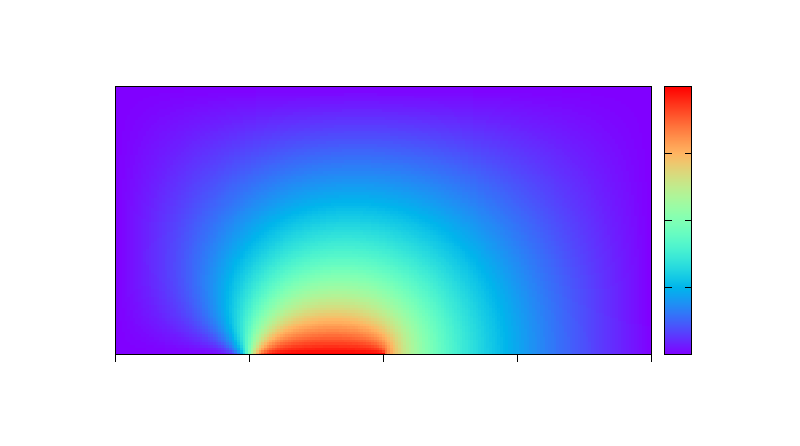
\includegraphics[width={368.50bp},height={198.40bp}]{figures/case_smith_hutton/smith_hutton_N201_Pe1.0e+00}}%
    \gplfronttext
  \end{picture}%
\endgroup
}
	% GNUPLOT: LaTeX picture with Postscript
\begingroup
  % Encoding inside the plot.  In the header of your document, this encoding
  % should to defined, e.g., by using
  % \usepackage[cp1252,<other encodings>]{inputenc}
  \inputencoding{cp1252}%
  \makeatletter
  \providecommand\color[2][]{%
    \GenericError{(gnuplot) \space\space\space\@spaces}{%
      Package color not loaded in conjunction with
      terminal option `colourtext'%
    }{See the gnuplot documentation for explanation.%
    }{Either use 'blacktext' in gnuplot or load the package
      color.sty in LaTeX.}%
    \renewcommand\color[2][]{}%
  }%
  \providecommand\includegraphics[2][]{%
    \GenericError{(gnuplot) \space\space\space\@spaces}{%
      Package graphicx or graphics not loaded%
    }{See the gnuplot documentation for explanation.%
    }{The gnuplot epslatex terminal needs graphicx.sty or graphics.sty.}%
    \renewcommand\includegraphics[2][]{}%
  }%
  \providecommand\rotatebox[2]{#2}%
  \@ifundefined{ifGPcolor}{%
    \newif\ifGPcolor
    \GPcolortrue
  }{}%
  \@ifundefined{ifGPblacktext}{%
    \newif\ifGPblacktext
    \GPblacktextfalse
  }{}%
  % define a \g@addto@macro without @ in the name:
  \let\gplgaddtomacro\g@addto@macro
  % define empty templates for all commands taking text:
  \gdef\gplbacktext{}%
  \gdef\gplfronttext{}%
  \makeatother
  \ifGPblacktext
    % no textcolor at all
    \def\colorrgb#1{}%
    \def\colorgray#1{}%
  \else
    % gray or color?
    \ifGPcolor
      \def\colorrgb#1{\color[rgb]{#1}}%
      \def\colorgray#1{\color[gray]{#1}}%
      \expandafter\def\csname LTw\endcsname{\color{white}}%
      \expandafter\def\csname LTb\endcsname{\color{black}}%
      \expandafter\def\csname LTa\endcsname{\color{black}}%
      \expandafter\def\csname LT0\endcsname{\color[rgb]{1,0,0}}%
      \expandafter\def\csname LT1\endcsname{\color[rgb]{0,1,0}}%
      \expandafter\def\csname LT2\endcsname{\color[rgb]{0,0,1}}%
      \expandafter\def\csname LT3\endcsname{\color[rgb]{1,0,1}}%
      \expandafter\def\csname LT4\endcsname{\color[rgb]{0,1,1}}%
      \expandafter\def\csname LT5\endcsname{\color[rgb]{1,1,0}}%
      \expandafter\def\csname LT6\endcsname{\color[rgb]{0,0,0}}%
      \expandafter\def\csname LT7\endcsname{\color[rgb]{1,0.3,0}}%
      \expandafter\def\csname LT8\endcsname{\color[rgb]{0.5,0.5,0.5}}%
    \else
      % gray
      \def\colorrgb#1{\color{black}}%
      \def\colorgray#1{\color[gray]{#1}}%
      \expandafter\def\csname LTw\endcsname{\color{white}}%
      \expandafter\def\csname LTb\endcsname{\color{black}}%
      \expandafter\def\csname LTa\endcsname{\color{black}}%
      \expandafter\def\csname LT0\endcsname{\color{black}}%
      \expandafter\def\csname LT1\endcsname{\color{black}}%
      \expandafter\def\csname LT2\endcsname{\color{black}}%
      \expandafter\def\csname LT3\endcsname{\color{black}}%
      \expandafter\def\csname LT4\endcsname{\color{black}}%
      \expandafter\def\csname LT5\endcsname{\color{black}}%
      \expandafter\def\csname LT6\endcsname{\color{black}}%
      \expandafter\def\csname LT7\endcsname{\color{black}}%
      \expandafter\def\csname LT8\endcsname{\color{black}}%
    \fi
  \fi
    \setlength{\unitlength}{0.0500bp}%
    \ifx\gptboxheight\undefined%
      \newlength{\gptboxheight}%
      \newlength{\gptboxwidth}%
      \newsavebox{\gptboxtext}%
    \fi%
    \setlength{\fboxrule}{0.5pt}%
    \setlength{\fboxsep}{1pt}%
    \definecolor{tbcol}{rgb}{1,1,1}%
\begin{picture}(7370.00,3968.00)%
    \gplgaddtomacro\gplbacktext{%
      \csname LTb\endcsname%%
      \put(814,719){\makebox(0,0)[r]{\strut{}0.0}}%
      \put(814,1234){\makebox(0,0)[r]{\strut{}0.2}}%
      \put(814,1748){\makebox(0,0)[r]{\strut{}0.4}}%
      \put(814,2263){\makebox(0,0)[r]{\strut{}0.6}}%
      \put(814,2777){\makebox(0,0)[r]{\strut{}0.8}}%
      \put(814,3292){\makebox(0,0)[r]{\strut{}1.0}}%
      \put(946,499){\makebox(0,0){\strut{}-1.0}}%
      \put(2233,499){\makebox(0,0){\strut{}-0.5}}%
      \put(3520,499){\makebox(0,0){\strut{}0.0}}%
      \put(4806,499){\makebox(0,0){\strut{}0.5}}%
      \put(6093,499){\makebox(0,0){\strut{}1.0}}%
    }%
    \gplgaddtomacro\gplfronttext{%
      \csname LTb\endcsname%%
      \put(209,2005){\rotatebox{-270}{\makebox(0,0){\strut{}$y \ (\mathrm{m})$}}}%
      \put(3519,169){\makebox(0,0){\strut{}$x \ (\mathrm{m})$}}%
      \csname LTb\endcsname%%
      \put(6611,719){\makebox(0,0)[l]{\strut{}0.0}}%
      \put(6611,1362){\makebox(0,0)[l]{\strut{}0.5}}%
      \put(6611,2005){\makebox(0,0)[l]{\strut{}1.0}}%
      \put(6611,2648){\makebox(0,0)[l]{\strut{}1.5}}%
      \put(6611,3292){\makebox(0,0)[l]{\strut{}2.0}}%
      \put(7073,2005){\rotatebox{-270}{\makebox(0,0){\strut{}$\phi$}}}%
      \put(3519,3622){\makebox(0,0){\strut{}\textbf{Smith--Hutton case} $(\mathrm{Pe} = 1)$}}%
    }%
    \gplbacktext
    \put(0,0){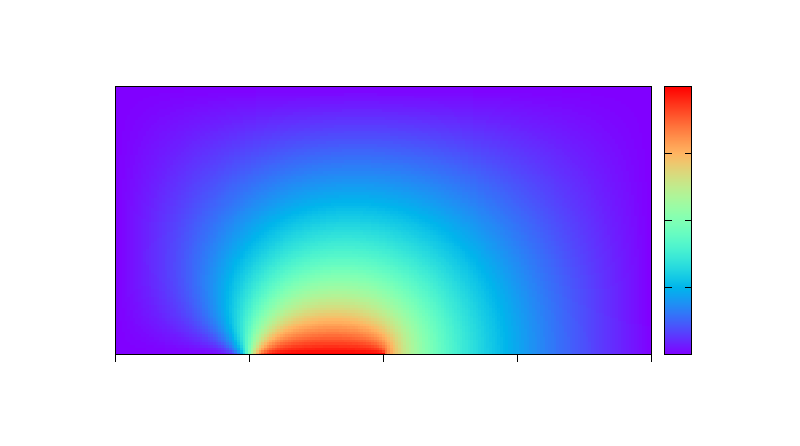
\includegraphics[width={368.50bp},height={198.40bp}]{figures/case_smith_hutton/smith_hutton_N201_Pe1.0e+00}}%
    \gplfronttext
  \end{picture}%
\endgroup

	\caption{Numerical solution the the Smith--Hutton case for $\rho / \Gamma = 1$.}
	\label{fig:smith_hutton_N201_Pe1.0e+00}
\end{figure}

\clearpage
Figures \ref{fig:smith_hutton_N201_Pe1.0e+01} and
\ref{fig:smith_hutton_N201_Pe1.0e+02} show the numerical solution to the
Smith--Hutton problem for $\rho / \Gamma = 10$ and $\rho / \Gamma = 100$,
respectively. Some differences between the solutions for $\rho / \Gamma = 1$ and
$\rho / \Gamma = 10$, although not too obvious, can be spotted. Clearly the
light blue, green and orange bands now occupy a larger portion of $\Omega$,
while the smooth transitions between them are still present. In contrast to the
$\rho / \Gamma = 10$ case, the change for $\rho / \Gamma = 100$ is more
apparent. Now the transition zones between the different color bands are
thinner, implying the diffusion process has lost strength with respect to the
transport process. However there is still diffusion, since the green band widens
along the streamlines.

\begin{figure}[ht]
	\centering
	%	\fbox{% GNUPLOT: LaTeX picture with Postscript
\documentclass{minimal}
% Set font size
\makeatletter
\def\@ptsize{1}
\InputIfFileExists{size11.clo}{}{%
   \GenericError{(gnuplot) \space\space\space\@spaces}{%
      Gnuplot Error: File `size11.clo' not found! Could not set font size%
   }{See the gnuplot documentation for explanation.%
   }{For using a font size a file `size<fontsize>.clo' has to exist.
        Falling back ^^Jto default fontsize 10pt.}%
  \def\@ptsize{0}
  \input{size10.clo}%
}%
\makeatother
% Load packages
\usepackage{calc}
\usepackage{graphicx}
\usepackage{color}
\usepackage[cp1252]{inputenc}
\makeatletter
% Select an appropriate default driver (from TeXLive graphics.cfg)
\begingroup
  \chardef\x=0 %
  % check pdfTeX
  \@ifundefined{pdfoutput}{}{%
    \ifcase\pdfoutput
    \else
      \chardef\x=1 %
    \fi
  }%
  % check VTeX
  \@ifundefined{OpMode}{}{%
    \chardef\x=2 %
  }%
\expandafter\endgroup
\ifcase\x
  % default case
  \PassOptionsToPackage{dvips}{geometry}
\or
  % pdfTeX is running in pdf mode
  \PassOptionsToPackage{pdftex}{geometry}
\else
  % VTeX is running
  \PassOptionsToPackage{vtex}{geometry}
\fi
\makeatother
% Set papersize
\usepackage[papersize={368.50bp,198.40bp},text={368.50bp,198.40bp}]{geometry}
% No page numbers and no paragraph indentation
\pagestyle{empty}
\setlength{\parindent}{0bp}%
% Load configuration file
\InputIfFileExists{gnuplot.cfg}{%
  \typeout{Using configuration file gnuplot.cfg}%
}{%
 \typeout{No configuration file gnuplot.cfg found.}%
}%
%
\begin{document}
\begingroup
  % Encoding inside the plot.  In the header of your document, this encoding
  % should to defined, e.g., by using
  % \usepackage[cp1252,<other encodings>]{inputenc}
  \inputencoding{cp1252}%
  \makeatletter
  \providecommand\color[2][]{%
    \GenericError{(gnuplot) \space\space\space\@spaces}{%
      Package color not loaded in conjunction with
      terminal option `colourtext'%
    }{See the gnuplot documentation for explanation.%
    }{Either use 'blacktext' in gnuplot or load the package
      color.sty in LaTeX.}%
    \renewcommand\color[2][]{}%
  }%
  \providecommand\includegraphics[2][]{%
    \GenericError{(gnuplot) \space\space\space\@spaces}{%
      Package graphicx or graphics not loaded%
    }{See the gnuplot documentation for explanation.%
    }{The gnuplot epslatex terminal needs graphicx.sty or graphics.sty.}%
    \renewcommand\includegraphics[2][]{}%
  }%
  \providecommand\rotatebox[2]{#2}%
  \@ifundefined{ifGPcolor}{%
    \newif\ifGPcolor
    \GPcolortrue
  }{}%
  \@ifundefined{ifGPblacktext}{%
    \newif\ifGPblacktext
    \GPblacktextfalse
  }{}%
  % define a \g@addto@macro without @ in the name:
  \let\gplgaddtomacro\g@addto@macro
  % define empty templates for all commands taking text:
  \gdef\gplbacktext{}%
  \gdef\gplfronttext{}%
  \makeatother
  \ifGPblacktext
    % no textcolor at all
    \def\colorrgb#1{}%
    \def\colorgray#1{}%
  \else
    % gray or color?
    \ifGPcolor
      \def\colorrgb#1{\color[rgb]{#1}}%
      \def\colorgray#1{\color[gray]{#1}}%
      \expandafter\def\csname LTw\endcsname{\color{white}}%
      \expandafter\def\csname LTb\endcsname{\color{black}}%
      \expandafter\def\csname LTa\endcsname{\color{black}}%
      \expandafter\def\csname LT0\endcsname{\color[rgb]{1,0,0}}%
      \expandafter\def\csname LT1\endcsname{\color[rgb]{0,1,0}}%
      \expandafter\def\csname LT2\endcsname{\color[rgb]{0,0,1}}%
      \expandafter\def\csname LT3\endcsname{\color[rgb]{1,0,1}}%
      \expandafter\def\csname LT4\endcsname{\color[rgb]{0,1,1}}%
      \expandafter\def\csname LT5\endcsname{\color[rgb]{1,1,0}}%
      \expandafter\def\csname LT6\endcsname{\color[rgb]{0,0,0}}%
      \expandafter\def\csname LT7\endcsname{\color[rgb]{1,0.3,0}}%
      \expandafter\def\csname LT8\endcsname{\color[rgb]{0.5,0.5,0.5}}%
    \else
      % gray
      \def\colorrgb#1{\color{black}}%
      \def\colorgray#1{\color[gray]{#1}}%
      \expandafter\def\csname LTw\endcsname{\color{white}}%
      \expandafter\def\csname LTb\endcsname{\color{black}}%
      \expandafter\def\csname LTa\endcsname{\color{black}}%
      \expandafter\def\csname LT0\endcsname{\color{black}}%
      \expandafter\def\csname LT1\endcsname{\color{black}}%
      \expandafter\def\csname LT2\endcsname{\color{black}}%
      \expandafter\def\csname LT3\endcsname{\color{black}}%
      \expandafter\def\csname LT4\endcsname{\color{black}}%
      \expandafter\def\csname LT5\endcsname{\color{black}}%
      \expandafter\def\csname LT6\endcsname{\color{black}}%
      \expandafter\def\csname LT7\endcsname{\color{black}}%
      \expandafter\def\csname LT8\endcsname{\color{black}}%
    \fi
  \fi
    \setlength{\unitlength}{0.0500bp}%
    \ifx\gptboxheight\undefined%
      \newlength{\gptboxheight}%
      \newlength{\gptboxwidth}%
      \newsavebox{\gptboxtext}%
    \fi%
    \setlength{\fboxrule}{0.5pt}%
    \setlength{\fboxsep}{1pt}%
    \definecolor{tbcol}{rgb}{1,1,1}%
\begin{picture}(7370.00,3968.00)%
    \gplgaddtomacro\gplbacktext{%
      \csname LTb\endcsname%%
      \put(814,733){\makebox(0,0)[r]{\strut{}0.0}}%
      \put(814,1242){\makebox(0,0)[r]{\strut{}0.2}}%
      \put(814,1751){\makebox(0,0)[r]{\strut{}0.4}}%
      \put(814,2260){\makebox(0,0)[r]{\strut{}0.6}}%
      \put(814,2769){\makebox(0,0)[r]{\strut{}0.8}}%
      \put(814,3278){\makebox(0,0)[r]{\strut{}1.0}}%
      \put(1009,513){\makebox(0,0){\strut{}-1.0}}%
      \put(2282,513){\makebox(0,0){\strut{}-0.5}}%
      \put(3554,513){\makebox(0,0){\strut{}0.0}}%
      \put(4827,513){\makebox(0,0){\strut{}0.5}}%
      \put(6099,513){\makebox(0,0){\strut{}1.0}}%
    }%
    \gplgaddtomacro\gplfronttext{%
      \csname LTb\endcsname%%
      \put(209,2005){\rotatebox{-270}{\makebox(0,0){\strut{}$y \ (\mathrm{m})$}}}%
      \put(3554,183){\makebox(0,0){\strut{}$x \ (\mathrm{m})$}}%
      \csname LTb\endcsname%%
      \put(6612,733){\makebox(0,0)[l]{\strut{}0.0}}%
      \put(6612,1369){\makebox(0,0)[l]{\strut{}0.5}}%
      \put(6612,2005){\makebox(0,0)[l]{\strut{}1.0}}%
      \put(6612,2641){\makebox(0,0)[l]{\strut{}1.5}}%
      \put(6612,3278){\makebox(0,0)[l]{\strut{}2.0}}%
      \put(7074,2005){\rotatebox{-270}{\makebox(0,0){\strut{}$\phi$}}}%
      \put(3554,3608){\makebox(0,0){\strut{}\textbf{Smith--Hutton case} $(\rho / \Gamma = 10)$}}%
    }%
    \gplbacktext
    \put(0,0){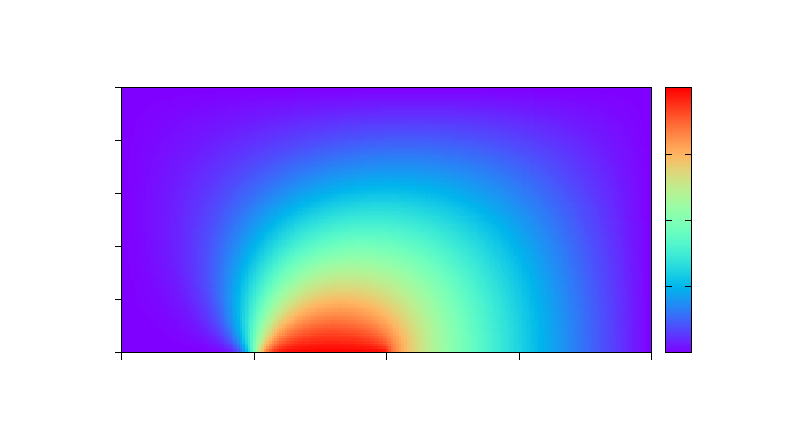
\includegraphics[width={368.50bp},height={198.40bp}]{smith_hutton_N201_Pe1.0e+01-inc}}%
    \gplfronttext
  \end{picture}%
\endgroup
\end{document}
}
	% GNUPLOT: LaTeX picture with Postscript
\documentclass{minimal}
% Set font size
\makeatletter
\def\@ptsize{1}
\InputIfFileExists{size11.clo}{}{%
   \GenericError{(gnuplot) \space\space\space\@spaces}{%
      Gnuplot Error: File `size11.clo' not found! Could not set font size%
   }{See the gnuplot documentation for explanation.%
   }{For using a font size a file `size<fontsize>.clo' has to exist.
        Falling back ^^Jto default fontsize 10pt.}%
  \def\@ptsize{0}
  \input{size10.clo}%
}%
\makeatother
% Load packages
\usepackage{calc}
\usepackage{graphicx}
\usepackage{color}
\usepackage[cp1252]{inputenc}
\makeatletter
% Select an appropriate default driver (from TeXLive graphics.cfg)
\begingroup
  \chardef\x=0 %
  % check pdfTeX
  \@ifundefined{pdfoutput}{}{%
    \ifcase\pdfoutput
    \else
      \chardef\x=1 %
    \fi
  }%
  % check VTeX
  \@ifundefined{OpMode}{}{%
    \chardef\x=2 %
  }%
\expandafter\endgroup
\ifcase\x
  % default case
  \PassOptionsToPackage{dvips}{geometry}
\or
  % pdfTeX is running in pdf mode
  \PassOptionsToPackage{pdftex}{geometry}
\else
  % VTeX is running
  \PassOptionsToPackage{vtex}{geometry}
\fi
\makeatother
% Set papersize
\usepackage[papersize={368.50bp,198.40bp},text={368.50bp,198.40bp}]{geometry}
% No page numbers and no paragraph indentation
\pagestyle{empty}
\setlength{\parindent}{0bp}%
% Load configuration file
\InputIfFileExists{gnuplot.cfg}{%
  \typeout{Using configuration file gnuplot.cfg}%
}{%
 \typeout{No configuration file gnuplot.cfg found.}%
}%
%
\begin{document}
\begingroup
  % Encoding inside the plot.  In the header of your document, this encoding
  % should to defined, e.g., by using
  % \usepackage[cp1252,<other encodings>]{inputenc}
  \inputencoding{cp1252}%
  \makeatletter
  \providecommand\color[2][]{%
    \GenericError{(gnuplot) \space\space\space\@spaces}{%
      Package color not loaded in conjunction with
      terminal option `colourtext'%
    }{See the gnuplot documentation for explanation.%
    }{Either use 'blacktext' in gnuplot or load the package
      color.sty in LaTeX.}%
    \renewcommand\color[2][]{}%
  }%
  \providecommand\includegraphics[2][]{%
    \GenericError{(gnuplot) \space\space\space\@spaces}{%
      Package graphicx or graphics not loaded%
    }{See the gnuplot documentation for explanation.%
    }{The gnuplot epslatex terminal needs graphicx.sty or graphics.sty.}%
    \renewcommand\includegraphics[2][]{}%
  }%
  \providecommand\rotatebox[2]{#2}%
  \@ifundefined{ifGPcolor}{%
    \newif\ifGPcolor
    \GPcolortrue
  }{}%
  \@ifundefined{ifGPblacktext}{%
    \newif\ifGPblacktext
    \GPblacktextfalse
  }{}%
  % define a \g@addto@macro without @ in the name:
  \let\gplgaddtomacro\g@addto@macro
  % define empty templates for all commands taking text:
  \gdef\gplbacktext{}%
  \gdef\gplfronttext{}%
  \makeatother
  \ifGPblacktext
    % no textcolor at all
    \def\colorrgb#1{}%
    \def\colorgray#1{}%
  \else
    % gray or color?
    \ifGPcolor
      \def\colorrgb#1{\color[rgb]{#1}}%
      \def\colorgray#1{\color[gray]{#1}}%
      \expandafter\def\csname LTw\endcsname{\color{white}}%
      \expandafter\def\csname LTb\endcsname{\color{black}}%
      \expandafter\def\csname LTa\endcsname{\color{black}}%
      \expandafter\def\csname LT0\endcsname{\color[rgb]{1,0,0}}%
      \expandafter\def\csname LT1\endcsname{\color[rgb]{0,1,0}}%
      \expandafter\def\csname LT2\endcsname{\color[rgb]{0,0,1}}%
      \expandafter\def\csname LT3\endcsname{\color[rgb]{1,0,1}}%
      \expandafter\def\csname LT4\endcsname{\color[rgb]{0,1,1}}%
      \expandafter\def\csname LT5\endcsname{\color[rgb]{1,1,0}}%
      \expandafter\def\csname LT6\endcsname{\color[rgb]{0,0,0}}%
      \expandafter\def\csname LT7\endcsname{\color[rgb]{1,0.3,0}}%
      \expandafter\def\csname LT8\endcsname{\color[rgb]{0.5,0.5,0.5}}%
    \else
      % gray
      \def\colorrgb#1{\color{black}}%
      \def\colorgray#1{\color[gray]{#1}}%
      \expandafter\def\csname LTw\endcsname{\color{white}}%
      \expandafter\def\csname LTb\endcsname{\color{black}}%
      \expandafter\def\csname LTa\endcsname{\color{black}}%
      \expandafter\def\csname LT0\endcsname{\color{black}}%
      \expandafter\def\csname LT1\endcsname{\color{black}}%
      \expandafter\def\csname LT2\endcsname{\color{black}}%
      \expandafter\def\csname LT3\endcsname{\color{black}}%
      \expandafter\def\csname LT4\endcsname{\color{black}}%
      \expandafter\def\csname LT5\endcsname{\color{black}}%
      \expandafter\def\csname LT6\endcsname{\color{black}}%
      \expandafter\def\csname LT7\endcsname{\color{black}}%
      \expandafter\def\csname LT8\endcsname{\color{black}}%
    \fi
  \fi
    \setlength{\unitlength}{0.0500bp}%
    \ifx\gptboxheight\undefined%
      \newlength{\gptboxheight}%
      \newlength{\gptboxwidth}%
      \newsavebox{\gptboxtext}%
    \fi%
    \setlength{\fboxrule}{0.5pt}%
    \setlength{\fboxsep}{1pt}%
    \definecolor{tbcol}{rgb}{1,1,1}%
\begin{picture}(7370.00,3968.00)%
    \gplgaddtomacro\gplbacktext{%
      \csname LTb\endcsname%%
      \put(814,733){\makebox(0,0)[r]{\strut{}0.0}}%
      \put(814,1242){\makebox(0,0)[r]{\strut{}0.2}}%
      \put(814,1751){\makebox(0,0)[r]{\strut{}0.4}}%
      \put(814,2260){\makebox(0,0)[r]{\strut{}0.6}}%
      \put(814,2769){\makebox(0,0)[r]{\strut{}0.8}}%
      \put(814,3278){\makebox(0,0)[r]{\strut{}1.0}}%
      \put(1009,513){\makebox(0,0){\strut{}-1.0}}%
      \put(2282,513){\makebox(0,0){\strut{}-0.5}}%
      \put(3554,513){\makebox(0,0){\strut{}0.0}}%
      \put(4827,513){\makebox(0,0){\strut{}0.5}}%
      \put(6099,513){\makebox(0,0){\strut{}1.0}}%
    }%
    \gplgaddtomacro\gplfronttext{%
      \csname LTb\endcsname%%
      \put(209,2005){\rotatebox{-270}{\makebox(0,0){\strut{}$y \ (\mathrm{m})$}}}%
      \put(3554,183){\makebox(0,0){\strut{}$x \ (\mathrm{m})$}}%
      \csname LTb\endcsname%%
      \put(6612,733){\makebox(0,0)[l]{\strut{}0.0}}%
      \put(6612,1369){\makebox(0,0)[l]{\strut{}0.5}}%
      \put(6612,2005){\makebox(0,0)[l]{\strut{}1.0}}%
      \put(6612,2641){\makebox(0,0)[l]{\strut{}1.5}}%
      \put(6612,3278){\makebox(0,0)[l]{\strut{}2.0}}%
      \put(7074,2005){\rotatebox{-270}{\makebox(0,0){\strut{}$\phi$}}}%
      \put(3554,3608){\makebox(0,0){\strut{}\textbf{Smith--Hutton case} $(\rho / \Gamma = 10)$}}%
    }%
    \gplbacktext
    \put(0,0){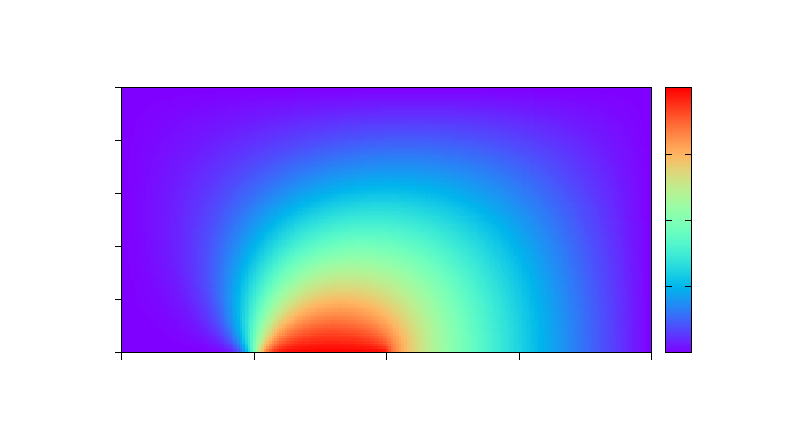
\includegraphics[width={368.50bp},height={198.40bp}]{smith_hutton_N201_Pe1.0e+01-inc}}%
    \gplfronttext
  \end{picture}%
\endgroup
\end{document}

	\caption{Numerical solution the the Smith--Hutton case for $\rho / \Gamma = 10$.}
	\label{fig:smith_hutton_N201_Pe1.0e+01}
	\vspace{1cm}
	% GNUPLOT: LaTeX picture with Postscript
\begingroup
  % Encoding inside the plot.  In the header of your document, this encoding
  % should to defined, e.g., by using
  % \usepackage[cp1252,<other encodings>]{inputenc}
  \inputencoding{cp1252}%
  \makeatletter
  \providecommand\color[2][]{%
    \GenericError{(gnuplot) \space\space\space\@spaces}{%
      Package color not loaded in conjunction with
      terminal option `colourtext'%
    }{See the gnuplot documentation for explanation.%
    }{Either use 'blacktext' in gnuplot or load the package
      color.sty in LaTeX.}%
    \renewcommand\color[2][]{}%
  }%
  \providecommand\includegraphics[2][]{%
    \GenericError{(gnuplot) \space\space\space\@spaces}{%
      Package graphicx or graphics not loaded%
    }{See the gnuplot documentation for explanation.%
    }{The gnuplot epslatex terminal needs graphicx.sty or graphics.sty.}%
    \renewcommand\includegraphics[2][]{}%
  }%
  \providecommand\rotatebox[2]{#2}%
  \@ifundefined{ifGPcolor}{%
    \newif\ifGPcolor
    \GPcolortrue
  }{}%
  \@ifundefined{ifGPblacktext}{%
    \newif\ifGPblacktext
    \GPblacktextfalse
  }{}%
  % define a \g@addto@macro without @ in the name:
  \let\gplgaddtomacro\g@addto@macro
  % define empty templates for all commands taking text:
  \gdef\gplbacktext{}%
  \gdef\gplfronttext{}%
  \makeatother
  \ifGPblacktext
    % no textcolor at all
    \def\colorrgb#1{}%
    \def\colorgray#1{}%
  \else
    % gray or color?
    \ifGPcolor
      \def\colorrgb#1{\color[rgb]{#1}}%
      \def\colorgray#1{\color[gray]{#1}}%
      \expandafter\def\csname LTw\endcsname{\color{white}}%
      \expandafter\def\csname LTb\endcsname{\color{black}}%
      \expandafter\def\csname LTa\endcsname{\color{black}}%
      \expandafter\def\csname LT0\endcsname{\color[rgb]{1,0,0}}%
      \expandafter\def\csname LT1\endcsname{\color[rgb]{0,1,0}}%
      \expandafter\def\csname LT2\endcsname{\color[rgb]{0,0,1}}%
      \expandafter\def\csname LT3\endcsname{\color[rgb]{1,0,1}}%
      \expandafter\def\csname LT4\endcsname{\color[rgb]{0,1,1}}%
      \expandafter\def\csname LT5\endcsname{\color[rgb]{1,1,0}}%
      \expandafter\def\csname LT6\endcsname{\color[rgb]{0,0,0}}%
      \expandafter\def\csname LT7\endcsname{\color[rgb]{1,0.3,0}}%
      \expandafter\def\csname LT8\endcsname{\color[rgb]{0.5,0.5,0.5}}%
    \else
      % gray
      \def\colorrgb#1{\color{black}}%
      \def\colorgray#1{\color[gray]{#1}}%
      \expandafter\def\csname LTw\endcsname{\color{white}}%
      \expandafter\def\csname LTb\endcsname{\color{black}}%
      \expandafter\def\csname LTa\endcsname{\color{black}}%
      \expandafter\def\csname LT0\endcsname{\color{black}}%
      \expandafter\def\csname LT1\endcsname{\color{black}}%
      \expandafter\def\csname LT2\endcsname{\color{black}}%
      \expandafter\def\csname LT3\endcsname{\color{black}}%
      \expandafter\def\csname LT4\endcsname{\color{black}}%
      \expandafter\def\csname LT5\endcsname{\color{black}}%
      \expandafter\def\csname LT6\endcsname{\color{black}}%
      \expandafter\def\csname LT7\endcsname{\color{black}}%
      \expandafter\def\csname LT8\endcsname{\color{black}}%
    \fi
  \fi
    \setlength{\unitlength}{0.0500bp}%
    \ifx\gptboxheight\undefined%
      \newlength{\gptboxheight}%
      \newlength{\gptboxwidth}%
      \newsavebox{\gptboxtext}%
    \fi%
    \setlength{\fboxrule}{0.5pt}%
    \setlength{\fboxsep}{1pt}%
    \definecolor{tbcol}{rgb}{1,1,1}%
\begin{picture}(7370.00,3968.00)%
    \gplgaddtomacro\gplbacktext{%
      \csname LTb\endcsname%%
      \put(814,719){\makebox(0,0)[r]{\strut{}0.0}}%
      \put(814,1234){\makebox(0,0)[r]{\strut{}0.2}}%
      \put(814,1748){\makebox(0,0)[r]{\strut{}0.4}}%
      \put(814,2263){\makebox(0,0)[r]{\strut{}0.6}}%
      \put(814,2777){\makebox(0,0)[r]{\strut{}0.8}}%
      \put(814,3292){\makebox(0,0)[r]{\strut{}1.0}}%
      \put(946,499){\makebox(0,0){\strut{}-1.0}}%
      \put(2233,499){\makebox(0,0){\strut{}-0.5}}%
      \put(3520,499){\makebox(0,0){\strut{}0.0}}%
      \put(4806,499){\makebox(0,0){\strut{}0.5}}%
      \put(6093,499){\makebox(0,0){\strut{}1.0}}%
    }%
    \gplgaddtomacro\gplfronttext{%
      \csname LTb\endcsname%%
      \put(209,2005){\rotatebox{-270}{\makebox(0,0){\strut{}$y \ (\mathrm{m})$}}}%
      \put(3519,169){\makebox(0,0){\strut{}$x \ (\mathrm{m})$}}%
      \csname LTb\endcsname%%
      \put(6611,719){\makebox(0,0)[l]{\strut{}0.0}}%
      \put(6611,1362){\makebox(0,0)[l]{\strut{}0.5}}%
      \put(6611,2005){\makebox(0,0)[l]{\strut{}1.0}}%
      \put(6611,2648){\makebox(0,0)[l]{\strut{}1.5}}%
      \put(6611,3292){\makebox(0,0)[l]{\strut{}2.0}}%
      \put(7073,2005){\rotatebox{-270}{\makebox(0,0){\strut{}$\phi$}}}%
      \put(3519,3622){\makebox(0,0){\strut{}\textbf{Smith--Hutton case} $(\mathrm{Pe} = 10^{2})$}}%
    }%
    \gplbacktext
    \put(0,0){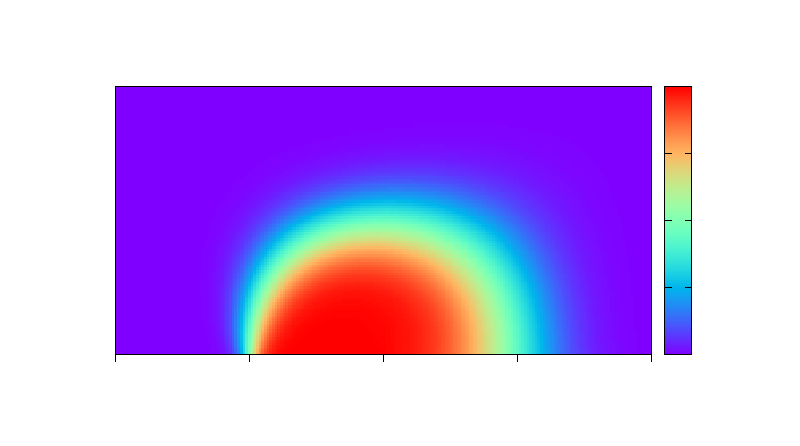
\includegraphics[width={368.50bp},height={198.40bp}]{figures/case_smith_hutton/smith_hutton_N201_Pe1.0e+02}}%
    \gplfronttext
  \end{picture}%
\endgroup

	\caption{Numerical solution the the Smith--Hutton case for $\rho / \Gamma = 10^2$.}
	\label{fig:smith_hutton_N201_Pe1.0e+02}
\end{figure}

% \begin{figure}[ht]
% 	\centering
% 	%	\fbox{% GNUPLOT: LaTeX picture with Postscript
\documentclass{minimal}
% Set font size
\makeatletter
\def\@ptsize{1}
\InputIfFileExists{size11.clo}{}{%
   \GenericError{(gnuplot) \space\space\space\@spaces}{%
      Gnuplot Error: File `size11.clo' not found! Could not set font size%
   }{See the gnuplot documentation for explanation.%
   }{For using a font size a file `size<fontsize>.clo' has to exist.
        Falling back ^^Jto default fontsize 10pt.}%
  \def\@ptsize{0}
  \input{size10.clo}%
}%
\makeatother
% Load packages
\usepackage{calc}
\usepackage{graphicx}
\usepackage{color}
\usepackage[cp1252]{inputenc}
\makeatletter
% Select an appropriate default driver (from TeXLive graphics.cfg)
\begingroup
  \chardef\x=0 %
  % check pdfTeX
  \@ifundefined{pdfoutput}{}{%
    \ifcase\pdfoutput
    \else
      \chardef\x=1 %
    \fi
  }%
  % check VTeX
  \@ifundefined{OpMode}{}{%
    \chardef\x=2 %
  }%
\expandafter\endgroup
\ifcase\x
  % default case
  \PassOptionsToPackage{dvips}{geometry}
\or
  % pdfTeX is running in pdf mode
  \PassOptionsToPackage{pdftex}{geometry}
\else
  % VTeX is running
  \PassOptionsToPackage{vtex}{geometry}
\fi
\makeatother
% Set papersize
\usepackage[papersize={368.50bp,198.40bp},text={368.50bp,198.40bp}]{geometry}
% No page numbers and no paragraph indentation
\pagestyle{empty}
\setlength{\parindent}{0bp}%
% Load configuration file
\InputIfFileExists{gnuplot.cfg}{%
  \typeout{Using configuration file gnuplot.cfg}%
}{%
 \typeout{No configuration file gnuplot.cfg found.}%
}%
%
\begin{document}
\begingroup
  % Encoding inside the plot.  In the header of your document, this encoding
  % should to defined, e.g., by using
  % \usepackage[cp1252,<other encodings>]{inputenc}
  \inputencoding{cp1252}%
  \makeatletter
  \providecommand\color[2][]{%
    \GenericError{(gnuplot) \space\space\space\@spaces}{%
      Package color not loaded in conjunction with
      terminal option `colourtext'%
    }{See the gnuplot documentation for explanation.%
    }{Either use 'blacktext' in gnuplot or load the package
      color.sty in LaTeX.}%
    \renewcommand\color[2][]{}%
  }%
  \providecommand\includegraphics[2][]{%
    \GenericError{(gnuplot) \space\space\space\@spaces}{%
      Package graphicx or graphics not loaded%
    }{See the gnuplot documentation for explanation.%
    }{The gnuplot epslatex terminal needs graphicx.sty or graphics.sty.}%
    \renewcommand\includegraphics[2][]{}%
  }%
  \providecommand\rotatebox[2]{#2}%
  \@ifundefined{ifGPcolor}{%
    \newif\ifGPcolor
    \GPcolortrue
  }{}%
  \@ifundefined{ifGPblacktext}{%
    \newif\ifGPblacktext
    \GPblacktextfalse
  }{}%
  % define a \g@addto@macro without @ in the name:
  \let\gplgaddtomacro\g@addto@macro
  % define empty templates for all commands taking text:
  \gdef\gplbacktext{}%
  \gdef\gplfronttext{}%
  \makeatother
  \ifGPblacktext
    % no textcolor at all
    \def\colorrgb#1{}%
    \def\colorgray#1{}%
  \else
    % gray or color?
    \ifGPcolor
      \def\colorrgb#1{\color[rgb]{#1}}%
      \def\colorgray#1{\color[gray]{#1}}%
      \expandafter\def\csname LTw\endcsname{\color{white}}%
      \expandafter\def\csname LTb\endcsname{\color{black}}%
      \expandafter\def\csname LTa\endcsname{\color{black}}%
      \expandafter\def\csname LT0\endcsname{\color[rgb]{1,0,0}}%
      \expandafter\def\csname LT1\endcsname{\color[rgb]{0,1,0}}%
      \expandafter\def\csname LT2\endcsname{\color[rgb]{0,0,1}}%
      \expandafter\def\csname LT3\endcsname{\color[rgb]{1,0,1}}%
      \expandafter\def\csname LT4\endcsname{\color[rgb]{0,1,1}}%
      \expandafter\def\csname LT5\endcsname{\color[rgb]{1,1,0}}%
      \expandafter\def\csname LT6\endcsname{\color[rgb]{0,0,0}}%
      \expandafter\def\csname LT7\endcsname{\color[rgb]{1,0.3,0}}%
      \expandafter\def\csname LT8\endcsname{\color[rgb]{0.5,0.5,0.5}}%
    \else
      % gray
      \def\colorrgb#1{\color{black}}%
      \def\colorgray#1{\color[gray]{#1}}%
      \expandafter\def\csname LTw\endcsname{\color{white}}%
      \expandafter\def\csname LTb\endcsname{\color{black}}%
      \expandafter\def\csname LTa\endcsname{\color{black}}%
      \expandafter\def\csname LT0\endcsname{\color{black}}%
      \expandafter\def\csname LT1\endcsname{\color{black}}%
      \expandafter\def\csname LT2\endcsname{\color{black}}%
      \expandafter\def\csname LT3\endcsname{\color{black}}%
      \expandafter\def\csname LT4\endcsname{\color{black}}%
      \expandafter\def\csname LT5\endcsname{\color{black}}%
      \expandafter\def\csname LT6\endcsname{\color{black}}%
      \expandafter\def\csname LT7\endcsname{\color{black}}%
      \expandafter\def\csname LT8\endcsname{\color{black}}%
    \fi
  \fi
    \setlength{\unitlength}{0.0500bp}%
    \ifx\gptboxheight\undefined%
      \newlength{\gptboxheight}%
      \newlength{\gptboxwidth}%
      \newsavebox{\gptboxtext}%
    \fi%
    \setlength{\fboxrule}{0.5pt}%
    \setlength{\fboxsep}{1pt}%
    \definecolor{tbcol}{rgb}{1,1,1}%
\begin{picture}(7370.00,3968.00)%
    \gplgaddtomacro\gplbacktext{%
      \csname LTb\endcsname%%
      \put(814,733){\makebox(0,0)[r]{\strut{}0.0}}%
      \put(814,1242){\makebox(0,0)[r]{\strut{}0.2}}%
      \put(814,1751){\makebox(0,0)[r]{\strut{}0.4}}%
      \put(814,2260){\makebox(0,0)[r]{\strut{}0.6}}%
      \put(814,2769){\makebox(0,0)[r]{\strut{}0.8}}%
      \put(814,3278){\makebox(0,0)[r]{\strut{}1.0}}%
      \put(1009,513){\makebox(0,0){\strut{}-1.0}}%
      \put(2282,513){\makebox(0,0){\strut{}-0.5}}%
      \put(3554,513){\makebox(0,0){\strut{}0.0}}%
      \put(4827,513){\makebox(0,0){\strut{}0.5}}%
      \put(6099,513){\makebox(0,0){\strut{}1.0}}%
    }%
    \gplgaddtomacro\gplfronttext{%
      \csname LTb\endcsname%%
      \put(209,2005){\rotatebox{-270}{\makebox(0,0){\strut{}$y \ (\mathrm{m})$}}}%
      \put(3554,183){\makebox(0,0){\strut{}$x \ (\mathrm{m})$}}%
      \csname LTb\endcsname%%
      \put(6612,733){\makebox(0,0)[l]{\strut{}0.0}}%
      \put(6612,1369){\makebox(0,0)[l]{\strut{}0.5}}%
      \put(6612,2005){\makebox(0,0)[l]{\strut{}1.0}}%
      \put(6612,2641){\makebox(0,0)[l]{\strut{}1.5}}%
      \put(6612,3278){\makebox(0,0)[l]{\strut{}2.0}}%
      \put(7074,2005){\rotatebox{-270}{\makebox(0,0){\strut{}$\phi$}}}%
      \put(3554,3608){\makebox(0,0){\strut{}\textbf{Smith--Hutton case} $(\rho / \Gamma = 10)$}}%
    }%
    \gplbacktext
    \put(0,0){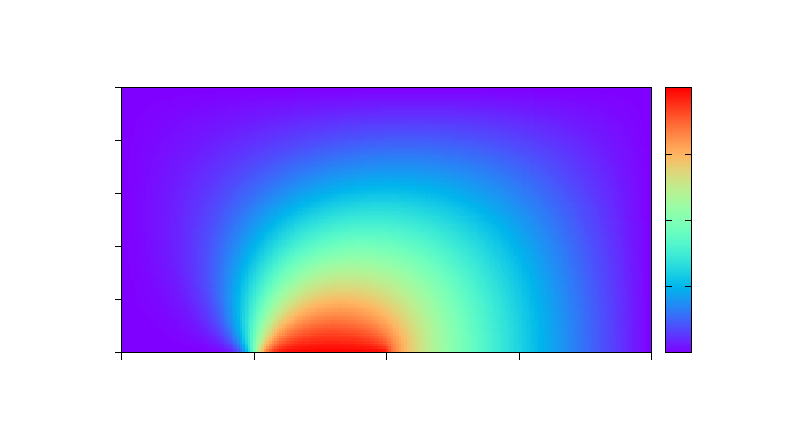
\includegraphics[width={368.50bp},height={198.40bp}]{smith_hutton_N201_Pe1.0e+01-inc}}%
    \gplfronttext
  \end{picture}%
\endgroup
\end{document}
}
% 	% GNUPLOT: LaTeX picture with Postscript
\documentclass{minimal}
% Set font size
\makeatletter
\def\@ptsize{1}
\InputIfFileExists{size11.clo}{}{%
   \GenericError{(gnuplot) \space\space\space\@spaces}{%
      Gnuplot Error: File `size11.clo' not found! Could not set font size%
   }{See the gnuplot documentation for explanation.%
   }{For using a font size a file `size<fontsize>.clo' has to exist.
        Falling back ^^Jto default fontsize 10pt.}%
  \def\@ptsize{0}
  \input{size10.clo}%
}%
\makeatother
% Load packages
\usepackage{calc}
\usepackage{graphicx}
\usepackage{color}
\usepackage[cp1252]{inputenc}
\makeatletter
% Select an appropriate default driver (from TeXLive graphics.cfg)
\begingroup
  \chardef\x=0 %
  % check pdfTeX
  \@ifundefined{pdfoutput}{}{%
    \ifcase\pdfoutput
    \else
      \chardef\x=1 %
    \fi
  }%
  % check VTeX
  \@ifundefined{OpMode}{}{%
    \chardef\x=2 %
  }%
\expandafter\endgroup
\ifcase\x
  % default case
  \PassOptionsToPackage{dvips}{geometry}
\or
  % pdfTeX is running in pdf mode
  \PassOptionsToPackage{pdftex}{geometry}
\else
  % VTeX is running
  \PassOptionsToPackage{vtex}{geometry}
\fi
\makeatother
% Set papersize
\usepackage[papersize={368.50bp,198.40bp},text={368.50bp,198.40bp}]{geometry}
% No page numbers and no paragraph indentation
\pagestyle{empty}
\setlength{\parindent}{0bp}%
% Load configuration file
\InputIfFileExists{gnuplot.cfg}{%
  \typeout{Using configuration file gnuplot.cfg}%
}{%
 \typeout{No configuration file gnuplot.cfg found.}%
}%
%
\begin{document}
\begingroup
  % Encoding inside the plot.  In the header of your document, this encoding
  % should to defined, e.g., by using
  % \usepackage[cp1252,<other encodings>]{inputenc}
  \inputencoding{cp1252}%
  \makeatletter
  \providecommand\color[2][]{%
    \GenericError{(gnuplot) \space\space\space\@spaces}{%
      Package color not loaded in conjunction with
      terminal option `colourtext'%
    }{See the gnuplot documentation for explanation.%
    }{Either use 'blacktext' in gnuplot or load the package
      color.sty in LaTeX.}%
    \renewcommand\color[2][]{}%
  }%
  \providecommand\includegraphics[2][]{%
    \GenericError{(gnuplot) \space\space\space\@spaces}{%
      Package graphicx or graphics not loaded%
    }{See the gnuplot documentation for explanation.%
    }{The gnuplot epslatex terminal needs graphicx.sty or graphics.sty.}%
    \renewcommand\includegraphics[2][]{}%
  }%
  \providecommand\rotatebox[2]{#2}%
  \@ifundefined{ifGPcolor}{%
    \newif\ifGPcolor
    \GPcolortrue
  }{}%
  \@ifundefined{ifGPblacktext}{%
    \newif\ifGPblacktext
    \GPblacktextfalse
  }{}%
  % define a \g@addto@macro without @ in the name:
  \let\gplgaddtomacro\g@addto@macro
  % define empty templates for all commands taking text:
  \gdef\gplbacktext{}%
  \gdef\gplfronttext{}%
  \makeatother
  \ifGPblacktext
    % no textcolor at all
    \def\colorrgb#1{}%
    \def\colorgray#1{}%
  \else
    % gray or color?
    \ifGPcolor
      \def\colorrgb#1{\color[rgb]{#1}}%
      \def\colorgray#1{\color[gray]{#1}}%
      \expandafter\def\csname LTw\endcsname{\color{white}}%
      \expandafter\def\csname LTb\endcsname{\color{black}}%
      \expandafter\def\csname LTa\endcsname{\color{black}}%
      \expandafter\def\csname LT0\endcsname{\color[rgb]{1,0,0}}%
      \expandafter\def\csname LT1\endcsname{\color[rgb]{0,1,0}}%
      \expandafter\def\csname LT2\endcsname{\color[rgb]{0,0,1}}%
      \expandafter\def\csname LT3\endcsname{\color[rgb]{1,0,1}}%
      \expandafter\def\csname LT4\endcsname{\color[rgb]{0,1,1}}%
      \expandafter\def\csname LT5\endcsname{\color[rgb]{1,1,0}}%
      \expandafter\def\csname LT6\endcsname{\color[rgb]{0,0,0}}%
      \expandafter\def\csname LT7\endcsname{\color[rgb]{1,0.3,0}}%
      \expandafter\def\csname LT8\endcsname{\color[rgb]{0.5,0.5,0.5}}%
    \else
      % gray
      \def\colorrgb#1{\color{black}}%
      \def\colorgray#1{\color[gray]{#1}}%
      \expandafter\def\csname LTw\endcsname{\color{white}}%
      \expandafter\def\csname LTb\endcsname{\color{black}}%
      \expandafter\def\csname LTa\endcsname{\color{black}}%
      \expandafter\def\csname LT0\endcsname{\color{black}}%
      \expandafter\def\csname LT1\endcsname{\color{black}}%
      \expandafter\def\csname LT2\endcsname{\color{black}}%
      \expandafter\def\csname LT3\endcsname{\color{black}}%
      \expandafter\def\csname LT4\endcsname{\color{black}}%
      \expandafter\def\csname LT5\endcsname{\color{black}}%
      \expandafter\def\csname LT6\endcsname{\color{black}}%
      \expandafter\def\csname LT7\endcsname{\color{black}}%
      \expandafter\def\csname LT8\endcsname{\color{black}}%
    \fi
  \fi
    \setlength{\unitlength}{0.0500bp}%
    \ifx\gptboxheight\undefined%
      \newlength{\gptboxheight}%
      \newlength{\gptboxwidth}%
      \newsavebox{\gptboxtext}%
    \fi%
    \setlength{\fboxrule}{0.5pt}%
    \setlength{\fboxsep}{1pt}%
    \definecolor{tbcol}{rgb}{1,1,1}%
\begin{picture}(7370.00,3968.00)%
    \gplgaddtomacro\gplbacktext{%
      \csname LTb\endcsname%%
      \put(814,733){\makebox(0,0)[r]{\strut{}0.0}}%
      \put(814,1242){\makebox(0,0)[r]{\strut{}0.2}}%
      \put(814,1751){\makebox(0,0)[r]{\strut{}0.4}}%
      \put(814,2260){\makebox(0,0)[r]{\strut{}0.6}}%
      \put(814,2769){\makebox(0,0)[r]{\strut{}0.8}}%
      \put(814,3278){\makebox(0,0)[r]{\strut{}1.0}}%
      \put(1009,513){\makebox(0,0){\strut{}-1.0}}%
      \put(2282,513){\makebox(0,0){\strut{}-0.5}}%
      \put(3554,513){\makebox(0,0){\strut{}0.0}}%
      \put(4827,513){\makebox(0,0){\strut{}0.5}}%
      \put(6099,513){\makebox(0,0){\strut{}1.0}}%
    }%
    \gplgaddtomacro\gplfronttext{%
      \csname LTb\endcsname%%
      \put(209,2005){\rotatebox{-270}{\makebox(0,0){\strut{}$y \ (\mathrm{m})$}}}%
      \put(3554,183){\makebox(0,0){\strut{}$x \ (\mathrm{m})$}}%
      \csname LTb\endcsname%%
      \put(6612,733){\makebox(0,0)[l]{\strut{}0.0}}%
      \put(6612,1369){\makebox(0,0)[l]{\strut{}0.5}}%
      \put(6612,2005){\makebox(0,0)[l]{\strut{}1.0}}%
      \put(6612,2641){\makebox(0,0)[l]{\strut{}1.5}}%
      \put(6612,3278){\makebox(0,0)[l]{\strut{}2.0}}%
      \put(7074,2005){\rotatebox{-270}{\makebox(0,0){\strut{}$\phi$}}}%
      \put(3554,3608){\makebox(0,0){\strut{}\textbf{Smith--Hutton case} $(\rho / \Gamma = 10)$}}%
    }%
    \gplbacktext
    \put(0,0){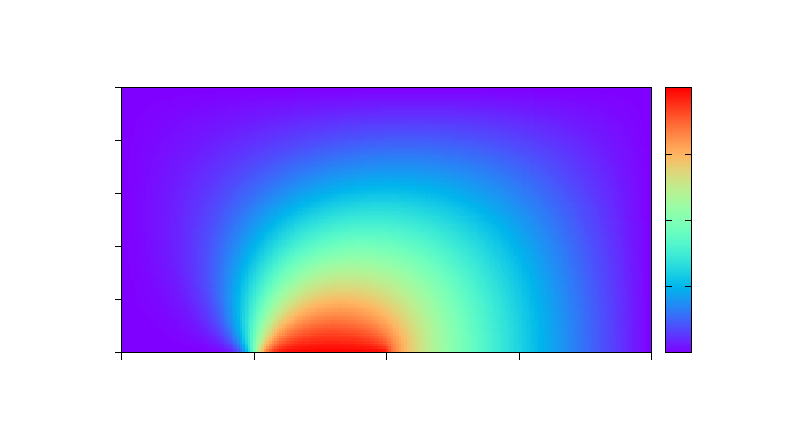
\includegraphics[width={368.50bp},height={198.40bp}]{smith_hutton_N201_Pe1.0e+01-inc}}%
    \gplfronttext
  \end{picture}%
\endgroup
\end{document}

% 	\caption{Numerical solution the the Smith--Hutton case for $\rho / \Gamma = 10$.}
% 	\label{fig:smith_hutton_N201_Pe1.0e+01}
% \end{figure}

% \begin{figure}[ht]
% 	\centering
% 	%	\fbox{% GNUPLOT: LaTeX picture with Postscript
\begingroup
  % Encoding inside the plot.  In the header of your document, this encoding
  % should to defined, e.g., by using
  % \usepackage[cp1252,<other encodings>]{inputenc}
  \inputencoding{cp1252}%
  \makeatletter
  \providecommand\color[2][]{%
    \GenericError{(gnuplot) \space\space\space\@spaces}{%
      Package color not loaded in conjunction with
      terminal option `colourtext'%
    }{See the gnuplot documentation for explanation.%
    }{Either use 'blacktext' in gnuplot or load the package
      color.sty in LaTeX.}%
    \renewcommand\color[2][]{}%
  }%
  \providecommand\includegraphics[2][]{%
    \GenericError{(gnuplot) \space\space\space\@spaces}{%
      Package graphicx or graphics not loaded%
    }{See the gnuplot documentation for explanation.%
    }{The gnuplot epslatex terminal needs graphicx.sty or graphics.sty.}%
    \renewcommand\includegraphics[2][]{}%
  }%
  \providecommand\rotatebox[2]{#2}%
  \@ifundefined{ifGPcolor}{%
    \newif\ifGPcolor
    \GPcolortrue
  }{}%
  \@ifundefined{ifGPblacktext}{%
    \newif\ifGPblacktext
    \GPblacktextfalse
  }{}%
  % define a \g@addto@macro without @ in the name:
  \let\gplgaddtomacro\g@addto@macro
  % define empty templates for all commands taking text:
  \gdef\gplbacktext{}%
  \gdef\gplfronttext{}%
  \makeatother
  \ifGPblacktext
    % no textcolor at all
    \def\colorrgb#1{}%
    \def\colorgray#1{}%
  \else
    % gray or color?
    \ifGPcolor
      \def\colorrgb#1{\color[rgb]{#1}}%
      \def\colorgray#1{\color[gray]{#1}}%
      \expandafter\def\csname LTw\endcsname{\color{white}}%
      \expandafter\def\csname LTb\endcsname{\color{black}}%
      \expandafter\def\csname LTa\endcsname{\color{black}}%
      \expandafter\def\csname LT0\endcsname{\color[rgb]{1,0,0}}%
      \expandafter\def\csname LT1\endcsname{\color[rgb]{0,1,0}}%
      \expandafter\def\csname LT2\endcsname{\color[rgb]{0,0,1}}%
      \expandafter\def\csname LT3\endcsname{\color[rgb]{1,0,1}}%
      \expandafter\def\csname LT4\endcsname{\color[rgb]{0,1,1}}%
      \expandafter\def\csname LT5\endcsname{\color[rgb]{1,1,0}}%
      \expandafter\def\csname LT6\endcsname{\color[rgb]{0,0,0}}%
      \expandafter\def\csname LT7\endcsname{\color[rgb]{1,0.3,0}}%
      \expandafter\def\csname LT8\endcsname{\color[rgb]{0.5,0.5,0.5}}%
    \else
      % gray
      \def\colorrgb#1{\color{black}}%
      \def\colorgray#1{\color[gray]{#1}}%
      \expandafter\def\csname LTw\endcsname{\color{white}}%
      \expandafter\def\csname LTb\endcsname{\color{black}}%
      \expandafter\def\csname LTa\endcsname{\color{black}}%
      \expandafter\def\csname LT0\endcsname{\color{black}}%
      \expandafter\def\csname LT1\endcsname{\color{black}}%
      \expandafter\def\csname LT2\endcsname{\color{black}}%
      \expandafter\def\csname LT3\endcsname{\color{black}}%
      \expandafter\def\csname LT4\endcsname{\color{black}}%
      \expandafter\def\csname LT5\endcsname{\color{black}}%
      \expandafter\def\csname LT6\endcsname{\color{black}}%
      \expandafter\def\csname LT7\endcsname{\color{black}}%
      \expandafter\def\csname LT8\endcsname{\color{black}}%
    \fi
  \fi
    \setlength{\unitlength}{0.0500bp}%
    \ifx\gptboxheight\undefined%
      \newlength{\gptboxheight}%
      \newlength{\gptboxwidth}%
      \newsavebox{\gptboxtext}%
    \fi%
    \setlength{\fboxrule}{0.5pt}%
    \setlength{\fboxsep}{1pt}%
    \definecolor{tbcol}{rgb}{1,1,1}%
\begin{picture}(7370.00,3968.00)%
    \gplgaddtomacro\gplbacktext{%
      \csname LTb\endcsname%%
      \put(814,719){\makebox(0,0)[r]{\strut{}0.0}}%
      \put(814,1234){\makebox(0,0)[r]{\strut{}0.2}}%
      \put(814,1748){\makebox(0,0)[r]{\strut{}0.4}}%
      \put(814,2263){\makebox(0,0)[r]{\strut{}0.6}}%
      \put(814,2777){\makebox(0,0)[r]{\strut{}0.8}}%
      \put(814,3292){\makebox(0,0)[r]{\strut{}1.0}}%
      \put(946,499){\makebox(0,0){\strut{}-1.0}}%
      \put(2233,499){\makebox(0,0){\strut{}-0.5}}%
      \put(3520,499){\makebox(0,0){\strut{}0.0}}%
      \put(4806,499){\makebox(0,0){\strut{}0.5}}%
      \put(6093,499){\makebox(0,0){\strut{}1.0}}%
    }%
    \gplgaddtomacro\gplfronttext{%
      \csname LTb\endcsname%%
      \put(209,2005){\rotatebox{-270}{\makebox(0,0){\strut{}$y \ (\mathrm{m})$}}}%
      \put(3519,169){\makebox(0,0){\strut{}$x \ (\mathrm{m})$}}%
      \csname LTb\endcsname%%
      \put(6611,719){\makebox(0,0)[l]{\strut{}0.0}}%
      \put(6611,1362){\makebox(0,0)[l]{\strut{}0.5}}%
      \put(6611,2005){\makebox(0,0)[l]{\strut{}1.0}}%
      \put(6611,2648){\makebox(0,0)[l]{\strut{}1.5}}%
      \put(6611,3292){\makebox(0,0)[l]{\strut{}2.0}}%
      \put(7073,2005){\rotatebox{-270}{\makebox(0,0){\strut{}$\phi$}}}%
      \put(3519,3622){\makebox(0,0){\strut{}\textbf{Smith--Hutton case} $(\mathrm{Pe} = 10^{2})$}}%
    }%
    \gplbacktext
    \put(0,0){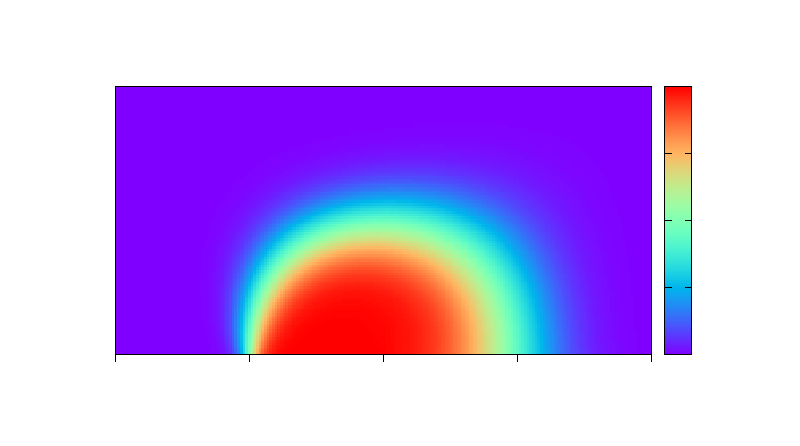
\includegraphics[width={368.50bp},height={198.40bp}]{figures/case_smith_hutton/smith_hutton_N201_Pe1.0e+02}}%
    \gplfronttext
  \end{picture}%
\endgroup
}
% 	% GNUPLOT: LaTeX picture with Postscript
\begingroup
  % Encoding inside the plot.  In the header of your document, this encoding
  % should to defined, e.g., by using
  % \usepackage[cp1252,<other encodings>]{inputenc}
  \inputencoding{cp1252}%
  \makeatletter
  \providecommand\color[2][]{%
    \GenericError{(gnuplot) \space\space\space\@spaces}{%
      Package color not loaded in conjunction with
      terminal option `colourtext'%
    }{See the gnuplot documentation for explanation.%
    }{Either use 'blacktext' in gnuplot or load the package
      color.sty in LaTeX.}%
    \renewcommand\color[2][]{}%
  }%
  \providecommand\includegraphics[2][]{%
    \GenericError{(gnuplot) \space\space\space\@spaces}{%
      Package graphicx or graphics not loaded%
    }{See the gnuplot documentation for explanation.%
    }{The gnuplot epslatex terminal needs graphicx.sty or graphics.sty.}%
    \renewcommand\includegraphics[2][]{}%
  }%
  \providecommand\rotatebox[2]{#2}%
  \@ifundefined{ifGPcolor}{%
    \newif\ifGPcolor
    \GPcolortrue
  }{}%
  \@ifundefined{ifGPblacktext}{%
    \newif\ifGPblacktext
    \GPblacktextfalse
  }{}%
  % define a \g@addto@macro without @ in the name:
  \let\gplgaddtomacro\g@addto@macro
  % define empty templates for all commands taking text:
  \gdef\gplbacktext{}%
  \gdef\gplfronttext{}%
  \makeatother
  \ifGPblacktext
    % no textcolor at all
    \def\colorrgb#1{}%
    \def\colorgray#1{}%
  \else
    % gray or color?
    \ifGPcolor
      \def\colorrgb#1{\color[rgb]{#1}}%
      \def\colorgray#1{\color[gray]{#1}}%
      \expandafter\def\csname LTw\endcsname{\color{white}}%
      \expandafter\def\csname LTb\endcsname{\color{black}}%
      \expandafter\def\csname LTa\endcsname{\color{black}}%
      \expandafter\def\csname LT0\endcsname{\color[rgb]{1,0,0}}%
      \expandafter\def\csname LT1\endcsname{\color[rgb]{0,1,0}}%
      \expandafter\def\csname LT2\endcsname{\color[rgb]{0,0,1}}%
      \expandafter\def\csname LT3\endcsname{\color[rgb]{1,0,1}}%
      \expandafter\def\csname LT4\endcsname{\color[rgb]{0,1,1}}%
      \expandafter\def\csname LT5\endcsname{\color[rgb]{1,1,0}}%
      \expandafter\def\csname LT6\endcsname{\color[rgb]{0,0,0}}%
      \expandafter\def\csname LT7\endcsname{\color[rgb]{1,0.3,0}}%
      \expandafter\def\csname LT8\endcsname{\color[rgb]{0.5,0.5,0.5}}%
    \else
      % gray
      \def\colorrgb#1{\color{black}}%
      \def\colorgray#1{\color[gray]{#1}}%
      \expandafter\def\csname LTw\endcsname{\color{white}}%
      \expandafter\def\csname LTb\endcsname{\color{black}}%
      \expandafter\def\csname LTa\endcsname{\color{black}}%
      \expandafter\def\csname LT0\endcsname{\color{black}}%
      \expandafter\def\csname LT1\endcsname{\color{black}}%
      \expandafter\def\csname LT2\endcsname{\color{black}}%
      \expandafter\def\csname LT3\endcsname{\color{black}}%
      \expandafter\def\csname LT4\endcsname{\color{black}}%
      \expandafter\def\csname LT5\endcsname{\color{black}}%
      \expandafter\def\csname LT6\endcsname{\color{black}}%
      \expandafter\def\csname LT7\endcsname{\color{black}}%
      \expandafter\def\csname LT8\endcsname{\color{black}}%
    \fi
  \fi
    \setlength{\unitlength}{0.0500bp}%
    \ifx\gptboxheight\undefined%
      \newlength{\gptboxheight}%
      \newlength{\gptboxwidth}%
      \newsavebox{\gptboxtext}%
    \fi%
    \setlength{\fboxrule}{0.5pt}%
    \setlength{\fboxsep}{1pt}%
    \definecolor{tbcol}{rgb}{1,1,1}%
\begin{picture}(7370.00,3968.00)%
    \gplgaddtomacro\gplbacktext{%
      \csname LTb\endcsname%%
      \put(814,719){\makebox(0,0)[r]{\strut{}0.0}}%
      \put(814,1234){\makebox(0,0)[r]{\strut{}0.2}}%
      \put(814,1748){\makebox(0,0)[r]{\strut{}0.4}}%
      \put(814,2263){\makebox(0,0)[r]{\strut{}0.6}}%
      \put(814,2777){\makebox(0,0)[r]{\strut{}0.8}}%
      \put(814,3292){\makebox(0,0)[r]{\strut{}1.0}}%
      \put(946,499){\makebox(0,0){\strut{}-1.0}}%
      \put(2233,499){\makebox(0,0){\strut{}-0.5}}%
      \put(3520,499){\makebox(0,0){\strut{}0.0}}%
      \put(4806,499){\makebox(0,0){\strut{}0.5}}%
      \put(6093,499){\makebox(0,0){\strut{}1.0}}%
    }%
    \gplgaddtomacro\gplfronttext{%
      \csname LTb\endcsname%%
      \put(209,2005){\rotatebox{-270}{\makebox(0,0){\strut{}$y \ (\mathrm{m})$}}}%
      \put(3519,169){\makebox(0,0){\strut{}$x \ (\mathrm{m})$}}%
      \csname LTb\endcsname%%
      \put(6611,719){\makebox(0,0)[l]{\strut{}0.0}}%
      \put(6611,1362){\makebox(0,0)[l]{\strut{}0.5}}%
      \put(6611,2005){\makebox(0,0)[l]{\strut{}1.0}}%
      \put(6611,2648){\makebox(0,0)[l]{\strut{}1.5}}%
      \put(6611,3292){\makebox(0,0)[l]{\strut{}2.0}}%
      \put(7073,2005){\rotatebox{-270}{\makebox(0,0){\strut{}$\phi$}}}%
      \put(3519,3622){\makebox(0,0){\strut{}\textbf{Smith--Hutton case} $(\mathrm{Pe} = 10^{2})$}}%
    }%
    \gplbacktext
    \put(0,0){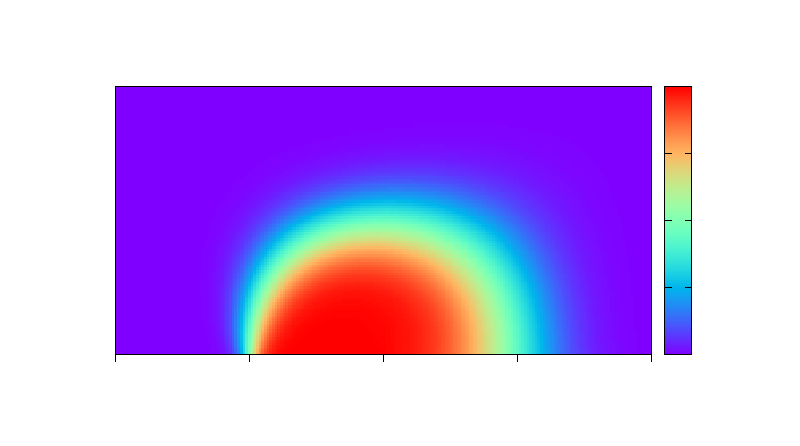
\includegraphics[width={368.50bp},height={198.40bp}]{figures/case_smith_hutton/smith_hutton_N201_Pe1.0e+02}}%
    \gplfronttext
  \end{picture}%
\endgroup

% 	\caption{Numerical solution the the Smith--Hutton case for $\rho / \Gamma = 10^2$.}
% 	\label{fig:smith_hutton_N201_Pe1.0e+02}
% \end{figure}


\clearpage
Figures \ref{fig:smith_hutton_N201_Pe1.0e+04} and
\ref{fig:smith_hutton_N201_Pe1.0e+09} show the numerical solution to the
Smith--Hutton case for $\rho / \Gamma = 10^4$ and $10^9$ respectively. There is
no apparent difference between two solution, what induces to think that for
$\rho / \Gamma > 10^4$ the solution stays approximately the same. There are
apparent discrepancies between the cases $\rho / \Gamma = 10^2$ and $\rho /
\Gamma = 10^4$. In the latter transport clearly takes over diffusion, as the
several color bands have approximately the same width, meaning diffusion has
much less strength than transport. 

\begin{figure}[ht]
	\centering
	% GNUPLOT: LaTeX picture with Postscript
\begingroup
  % Encoding inside the plot.  In the header of your document, this encoding
  % should to defined, e.g., by using
  % \usepackage[cp1252,<other encodings>]{inputenc}
  \inputencoding{cp1252}%
  \makeatletter
  \providecommand\color[2][]{%
    \GenericError{(gnuplot) \space\space\space\@spaces}{%
      Package color not loaded in conjunction with
      terminal option `colourtext'%
    }{See the gnuplot documentation for explanation.%
    }{Either use 'blacktext' in gnuplot or load the package
      color.sty in LaTeX.}%
    \renewcommand\color[2][]{}%
  }%
  \providecommand\includegraphics[2][]{%
    \GenericError{(gnuplot) \space\space\space\@spaces}{%
      Package graphicx or graphics not loaded%
    }{See the gnuplot documentation for explanation.%
    }{The gnuplot epslatex terminal needs graphicx.sty or graphics.sty.}%
    \renewcommand\includegraphics[2][]{}%
  }%
  \providecommand\rotatebox[2]{#2}%
  \@ifundefined{ifGPcolor}{%
    \newif\ifGPcolor
    \GPcolortrue
  }{}%
  \@ifundefined{ifGPblacktext}{%
    \newif\ifGPblacktext
    \GPblacktextfalse
  }{}%
  % define a \g@addto@macro without @ in the name:
  \let\gplgaddtomacro\g@addto@macro
  % define empty templates for all commands taking text:
  \gdef\gplbacktext{}%
  \gdef\gplfronttext{}%
  \makeatother
  \ifGPblacktext
    % no textcolor at all
    \def\colorrgb#1{}%
    \def\colorgray#1{}%
  \else
    % gray or color?
    \ifGPcolor
      \def\colorrgb#1{\color[rgb]{#1}}%
      \def\colorgray#1{\color[gray]{#1}}%
      \expandafter\def\csname LTw\endcsname{\color{white}}%
      \expandafter\def\csname LTb\endcsname{\color{black}}%
      \expandafter\def\csname LTa\endcsname{\color{black}}%
      \expandafter\def\csname LT0\endcsname{\color[rgb]{1,0,0}}%
      \expandafter\def\csname LT1\endcsname{\color[rgb]{0,1,0}}%
      \expandafter\def\csname LT2\endcsname{\color[rgb]{0,0,1}}%
      \expandafter\def\csname LT3\endcsname{\color[rgb]{1,0,1}}%
      \expandafter\def\csname LT4\endcsname{\color[rgb]{0,1,1}}%
      \expandafter\def\csname LT5\endcsname{\color[rgb]{1,1,0}}%
      \expandafter\def\csname LT6\endcsname{\color[rgb]{0,0,0}}%
      \expandafter\def\csname LT7\endcsname{\color[rgb]{1,0.3,0}}%
      \expandafter\def\csname LT8\endcsname{\color[rgb]{0.5,0.5,0.5}}%
    \else
      % gray
      \def\colorrgb#1{\color{black}}%
      \def\colorgray#1{\color[gray]{#1}}%
      \expandafter\def\csname LTw\endcsname{\color{white}}%
      \expandafter\def\csname LTb\endcsname{\color{black}}%
      \expandafter\def\csname LTa\endcsname{\color{black}}%
      \expandafter\def\csname LT0\endcsname{\color{black}}%
      \expandafter\def\csname LT1\endcsname{\color{black}}%
      \expandafter\def\csname LT2\endcsname{\color{black}}%
      \expandafter\def\csname LT3\endcsname{\color{black}}%
      \expandafter\def\csname LT4\endcsname{\color{black}}%
      \expandafter\def\csname LT5\endcsname{\color{black}}%
      \expandafter\def\csname LT6\endcsname{\color{black}}%
      \expandafter\def\csname LT7\endcsname{\color{black}}%
      \expandafter\def\csname LT8\endcsname{\color{black}}%
    \fi
  \fi
    \setlength{\unitlength}{0.0500bp}%
    \ifx\gptboxheight\undefined%
      \newlength{\gptboxheight}%
      \newlength{\gptboxwidth}%
      \newsavebox{\gptboxtext}%
    \fi%
    \setlength{\fboxrule}{0.5pt}%
    \setlength{\fboxsep}{1pt}%
    \definecolor{tbcol}{rgb}{1,1,1}%
\begin{picture}(7370.00,3968.00)%
    \gplgaddtomacro\gplbacktext{%
      \csname LTb\endcsname%%
      \put(814,719){\makebox(0,0)[r]{\strut{}0.0}}%
      \put(814,1234){\makebox(0,0)[r]{\strut{}0.2}}%
      \put(814,1748){\makebox(0,0)[r]{\strut{}0.4}}%
      \put(814,2263){\makebox(0,0)[r]{\strut{}0.6}}%
      \put(814,2777){\makebox(0,0)[r]{\strut{}0.8}}%
      \put(814,3292){\makebox(0,0)[r]{\strut{}1.0}}%
      \put(946,499){\makebox(0,0){\strut{}-1.0}}%
      \put(2233,499){\makebox(0,0){\strut{}-0.5}}%
      \put(3520,499){\makebox(0,0){\strut{}0.0}}%
      \put(4806,499){\makebox(0,0){\strut{}0.5}}%
      \put(6093,499){\makebox(0,0){\strut{}1.0}}%
    }%
    \gplgaddtomacro\gplfronttext{%
      \csname LTb\endcsname%%
      \put(209,2005){\rotatebox{-270}{\makebox(0,0){\strut{}$y \ (\mathrm{m})$}}}%
      \put(3519,169){\makebox(0,0){\strut{}$x \ (\mathrm{m})$}}%
      \csname LTb\endcsname%%
      \put(6611,719){\makebox(0,0)[l]{\strut{}0.0}}%
      \put(6611,1362){\makebox(0,0)[l]{\strut{}0.5}}%
      \put(6611,2005){\makebox(0,0)[l]{\strut{}1.0}}%
      \put(6611,2648){\makebox(0,0)[l]{\strut{}1.5}}%
      \put(6611,3292){\makebox(0,0)[l]{\strut{}2.0}}%
      \put(7073,2005){\rotatebox{-270}{\makebox(0,0){\strut{}$\phi$}}}%
      \put(3519,3622){\makebox(0,0){\strut{}\textbf{Smith--Hutton case} $(\mathrm{Pe} = 10^{4})$}}%
    }%
    \gplbacktext
    \put(0,0){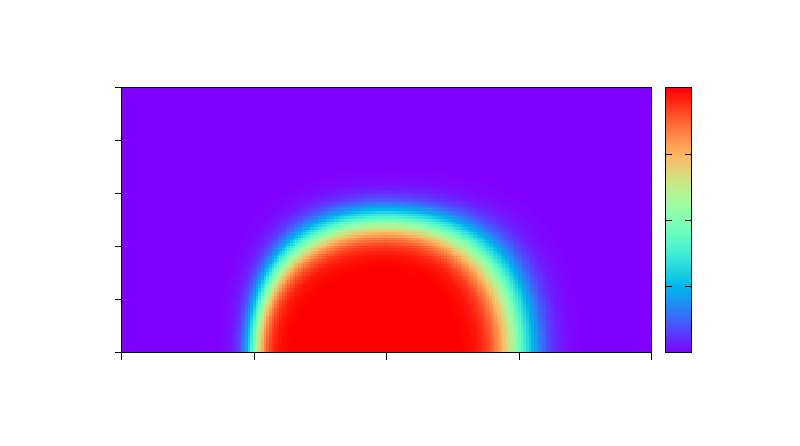
\includegraphics[width={368.50bp},height={198.40bp}]{figures/case_smith_hutton/smith_hutton_N201_Pe1.0e+04}}%
    \gplfronttext
  \end{picture}%
\endgroup

	\caption{Numerical solution the the Smith--Hutton case for $\rho / \Gamma = 10^4$.}
	\label{fig:smith_hutton_N201_Pe1.0e+04}
	\vspace{1cm}
	% GNUPLOT: LaTeX picture with Postscript
\begingroup
  % Encoding inside the plot.  In the header of your document, this encoding
  % should to defined, e.g., by using
  % \usepackage[cp1252,<other encodings>]{inputenc}
  \inputencoding{cp1252}%
  \makeatletter
  \providecommand\color[2][]{%
    \GenericError{(gnuplot) \space\space\space\@spaces}{%
      Package color not loaded in conjunction with
      terminal option `colourtext'%
    }{See the gnuplot documentation for explanation.%
    }{Either use 'blacktext' in gnuplot or load the package
      color.sty in LaTeX.}%
    \renewcommand\color[2][]{}%
  }%
  \providecommand\includegraphics[2][]{%
    \GenericError{(gnuplot) \space\space\space\@spaces}{%
      Package graphicx or graphics not loaded%
    }{See the gnuplot documentation for explanation.%
    }{The gnuplot epslatex terminal needs graphicx.sty or graphics.sty.}%
    \renewcommand\includegraphics[2][]{}%
  }%
  \providecommand\rotatebox[2]{#2}%
  \@ifundefined{ifGPcolor}{%
    \newif\ifGPcolor
    \GPcolortrue
  }{}%
  \@ifundefined{ifGPblacktext}{%
    \newif\ifGPblacktext
    \GPblacktextfalse
  }{}%
  % define a \g@addto@macro without @ in the name:
  \let\gplgaddtomacro\g@addto@macro
  % define empty templates for all commands taking text:
  \gdef\gplbacktext{}%
  \gdef\gplfronttext{}%
  \makeatother
  \ifGPblacktext
    % no textcolor at all
    \def\colorrgb#1{}%
    \def\colorgray#1{}%
  \else
    % gray or color?
    \ifGPcolor
      \def\colorrgb#1{\color[rgb]{#1}}%
      \def\colorgray#1{\color[gray]{#1}}%
      \expandafter\def\csname LTw\endcsname{\color{white}}%
      \expandafter\def\csname LTb\endcsname{\color{black}}%
      \expandafter\def\csname LTa\endcsname{\color{black}}%
      \expandafter\def\csname LT0\endcsname{\color[rgb]{1,0,0}}%
      \expandafter\def\csname LT1\endcsname{\color[rgb]{0,1,0}}%
      \expandafter\def\csname LT2\endcsname{\color[rgb]{0,0,1}}%
      \expandafter\def\csname LT3\endcsname{\color[rgb]{1,0,1}}%
      \expandafter\def\csname LT4\endcsname{\color[rgb]{0,1,1}}%
      \expandafter\def\csname LT5\endcsname{\color[rgb]{1,1,0}}%
      \expandafter\def\csname LT6\endcsname{\color[rgb]{0,0,0}}%
      \expandafter\def\csname LT7\endcsname{\color[rgb]{1,0.3,0}}%
      \expandafter\def\csname LT8\endcsname{\color[rgb]{0.5,0.5,0.5}}%
    \else
      % gray
      \def\colorrgb#1{\color{black}}%
      \def\colorgray#1{\color[gray]{#1}}%
      \expandafter\def\csname LTw\endcsname{\color{white}}%
      \expandafter\def\csname LTb\endcsname{\color{black}}%
      \expandafter\def\csname LTa\endcsname{\color{black}}%
      \expandafter\def\csname LT0\endcsname{\color{black}}%
      \expandafter\def\csname LT1\endcsname{\color{black}}%
      \expandafter\def\csname LT2\endcsname{\color{black}}%
      \expandafter\def\csname LT3\endcsname{\color{black}}%
      \expandafter\def\csname LT4\endcsname{\color{black}}%
      \expandafter\def\csname LT5\endcsname{\color{black}}%
      \expandafter\def\csname LT6\endcsname{\color{black}}%
      \expandafter\def\csname LT7\endcsname{\color{black}}%
      \expandafter\def\csname LT8\endcsname{\color{black}}%
    \fi
  \fi
    \setlength{\unitlength}{0.0500bp}%
    \ifx\gptboxheight\undefined%
      \newlength{\gptboxheight}%
      \newlength{\gptboxwidth}%
      \newsavebox{\gptboxtext}%
    \fi%
    \setlength{\fboxrule}{0.5pt}%
    \setlength{\fboxsep}{1pt}%
    \definecolor{tbcol}{rgb}{1,1,1}%
\begin{picture}(7370.00,3968.00)%
    \gplgaddtomacro\gplbacktext{%
      \csname LTb\endcsname%%
      \put(814,733){\makebox(0,0)[r]{\strut{}$0$}}%
      \put(814,1242){\makebox(0,0)[r]{\strut{}$0.2$}}%
      \put(814,1751){\makebox(0,0)[r]{\strut{}$0.4$}}%
      \put(814,2260){\makebox(0,0)[r]{\strut{}$0.6$}}%
      \put(814,2769){\makebox(0,0)[r]{\strut{}$0.8$}}%
      \put(814,3278){\makebox(0,0)[r]{\strut{}$1$}}%
      \put(1009,513){\makebox(0,0){\strut{}-1.0}}%
      \put(2282,513){\makebox(0,0){\strut{}-0.5}}%
      \put(3554,513){\makebox(0,0){\strut{}0.0}}%
      \put(4827,513){\makebox(0,0){\strut{}0.5}}%
      \put(6099,513){\makebox(0,0){\strut{}1.0}}%
    }%
    \gplgaddtomacro\gplfronttext{%
      \csname LTb\endcsname%%
      \put(209,2005){\rotatebox{-270}{\makebox(0,0){\strut{}$y \ (\mathrm{m})$}}}%
      \put(3554,183){\makebox(0,0){\strut{}$x \ (\mathrm{m})$}}%
      \csname LTb\endcsname%%
      \put(6612,733){\makebox(0,0)[l]{\strut{}0.0}}%
      \put(6612,1369){\makebox(0,0)[l]{\strut{}0.5}}%
      \put(6612,2005){\makebox(0,0)[l]{\strut{}1.0}}%
      \put(6612,2641){\makebox(0,0)[l]{\strut{}1.5}}%
      \put(6612,3278){\makebox(0,0)[l]{\strut{}2.0}}%
      \put(7074,2005){\rotatebox{-270}{\makebox(0,0){\strut{}$\phi$}}}%
      \put(3554,3608){\makebox(0,0){\strut{}\textbf{Smith--Hutton case} $(\rho / \Gamma = 10^{9})$}}%
    }%
    \gplbacktext
    \put(0,0){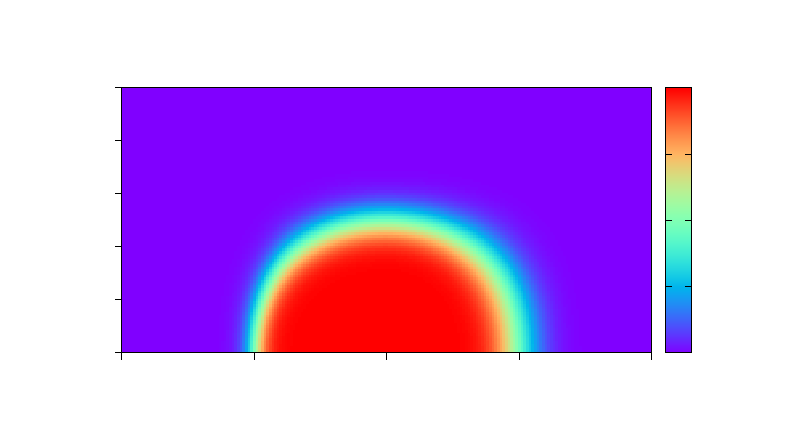
\includegraphics[width={368.50bp},height={198.40bp}]{figures/case_smith_hutton/smith_hutton_N201_Pe1.0e+09}}%
    \gplfronttext
  \end{picture}%
\endgroup

	\caption{Numerical solution the the Smith--Hutton case for $\rho / \Gamma = 10^9$.}
	\label{fig:smith_hutton_N201_Pe1.0e+09}
\end{figure}


% \begin{figure}[ht]
% 	\centering
% 	%	\fbox{% GNUPLOT: LaTeX picture with Postscript
\begingroup
  % Encoding inside the plot.  In the header of your document, this encoding
  % should to defined, e.g., by using
  % \usepackage[cp1252,<other encodings>]{inputenc}
  \inputencoding{cp1252}%
  \makeatletter
  \providecommand\color[2][]{%
    \GenericError{(gnuplot) \space\space\space\@spaces}{%
      Package color not loaded in conjunction with
      terminal option `colourtext'%
    }{See the gnuplot documentation for explanation.%
    }{Either use 'blacktext' in gnuplot or load the package
      color.sty in LaTeX.}%
    \renewcommand\color[2][]{}%
  }%
  \providecommand\includegraphics[2][]{%
    \GenericError{(gnuplot) \space\space\space\@spaces}{%
      Package graphicx or graphics not loaded%
    }{See the gnuplot documentation for explanation.%
    }{The gnuplot epslatex terminal needs graphicx.sty or graphics.sty.}%
    \renewcommand\includegraphics[2][]{}%
  }%
  \providecommand\rotatebox[2]{#2}%
  \@ifundefined{ifGPcolor}{%
    \newif\ifGPcolor
    \GPcolortrue
  }{}%
  \@ifundefined{ifGPblacktext}{%
    \newif\ifGPblacktext
    \GPblacktextfalse
  }{}%
  % define a \g@addto@macro without @ in the name:
  \let\gplgaddtomacro\g@addto@macro
  % define empty templates for all commands taking text:
  \gdef\gplbacktext{}%
  \gdef\gplfronttext{}%
  \makeatother
  \ifGPblacktext
    % no textcolor at all
    \def\colorrgb#1{}%
    \def\colorgray#1{}%
  \else
    % gray or color?
    \ifGPcolor
      \def\colorrgb#1{\color[rgb]{#1}}%
      \def\colorgray#1{\color[gray]{#1}}%
      \expandafter\def\csname LTw\endcsname{\color{white}}%
      \expandafter\def\csname LTb\endcsname{\color{black}}%
      \expandafter\def\csname LTa\endcsname{\color{black}}%
      \expandafter\def\csname LT0\endcsname{\color[rgb]{1,0,0}}%
      \expandafter\def\csname LT1\endcsname{\color[rgb]{0,1,0}}%
      \expandafter\def\csname LT2\endcsname{\color[rgb]{0,0,1}}%
      \expandafter\def\csname LT3\endcsname{\color[rgb]{1,0,1}}%
      \expandafter\def\csname LT4\endcsname{\color[rgb]{0,1,1}}%
      \expandafter\def\csname LT5\endcsname{\color[rgb]{1,1,0}}%
      \expandafter\def\csname LT6\endcsname{\color[rgb]{0,0,0}}%
      \expandafter\def\csname LT7\endcsname{\color[rgb]{1,0.3,0}}%
      \expandafter\def\csname LT8\endcsname{\color[rgb]{0.5,0.5,0.5}}%
    \else
      % gray
      \def\colorrgb#1{\color{black}}%
      \def\colorgray#1{\color[gray]{#1}}%
      \expandafter\def\csname LTw\endcsname{\color{white}}%
      \expandafter\def\csname LTb\endcsname{\color{black}}%
      \expandafter\def\csname LTa\endcsname{\color{black}}%
      \expandafter\def\csname LT0\endcsname{\color{black}}%
      \expandafter\def\csname LT1\endcsname{\color{black}}%
      \expandafter\def\csname LT2\endcsname{\color{black}}%
      \expandafter\def\csname LT3\endcsname{\color{black}}%
      \expandafter\def\csname LT4\endcsname{\color{black}}%
      \expandafter\def\csname LT5\endcsname{\color{black}}%
      \expandafter\def\csname LT6\endcsname{\color{black}}%
      \expandafter\def\csname LT7\endcsname{\color{black}}%
      \expandafter\def\csname LT8\endcsname{\color{black}}%
    \fi
  \fi
    \setlength{\unitlength}{0.0500bp}%
    \ifx\gptboxheight\undefined%
      \newlength{\gptboxheight}%
      \newlength{\gptboxwidth}%
      \newsavebox{\gptboxtext}%
    \fi%
    \setlength{\fboxrule}{0.5pt}%
    \setlength{\fboxsep}{1pt}%
    \definecolor{tbcol}{rgb}{1,1,1}%
\begin{picture}(7370.00,3968.00)%
    \gplgaddtomacro\gplbacktext{%
      \csname LTb\endcsname%%
      \put(814,719){\makebox(0,0)[r]{\strut{}0.0}}%
      \put(814,1234){\makebox(0,0)[r]{\strut{}0.2}}%
      \put(814,1748){\makebox(0,0)[r]{\strut{}0.4}}%
      \put(814,2263){\makebox(0,0)[r]{\strut{}0.6}}%
      \put(814,2777){\makebox(0,0)[r]{\strut{}0.8}}%
      \put(814,3292){\makebox(0,0)[r]{\strut{}1.0}}%
      \put(946,499){\makebox(0,0){\strut{}-1.0}}%
      \put(2233,499){\makebox(0,0){\strut{}-0.5}}%
      \put(3520,499){\makebox(0,0){\strut{}0.0}}%
      \put(4806,499){\makebox(0,0){\strut{}0.5}}%
      \put(6093,499){\makebox(0,0){\strut{}1.0}}%
    }%
    \gplgaddtomacro\gplfronttext{%
      \csname LTb\endcsname%%
      \put(209,2005){\rotatebox{-270}{\makebox(0,0){\strut{}$y \ (\mathrm{m})$}}}%
      \put(3519,169){\makebox(0,0){\strut{}$x \ (\mathrm{m})$}}%
      \csname LTb\endcsname%%
      \put(6611,719){\makebox(0,0)[l]{\strut{}0.0}}%
      \put(6611,1362){\makebox(0,0)[l]{\strut{}0.5}}%
      \put(6611,2005){\makebox(0,0)[l]{\strut{}1.0}}%
      \put(6611,2648){\makebox(0,0)[l]{\strut{}1.5}}%
      \put(6611,3292){\makebox(0,0)[l]{\strut{}2.0}}%
      \put(7073,2005){\rotatebox{-270}{\makebox(0,0){\strut{}$\phi$}}}%
      \put(3519,3622){\makebox(0,0){\strut{}\textbf{Smith--Hutton case} $(\mathrm{Pe} = 10^{4})$}}%
    }%
    \gplbacktext
    \put(0,0){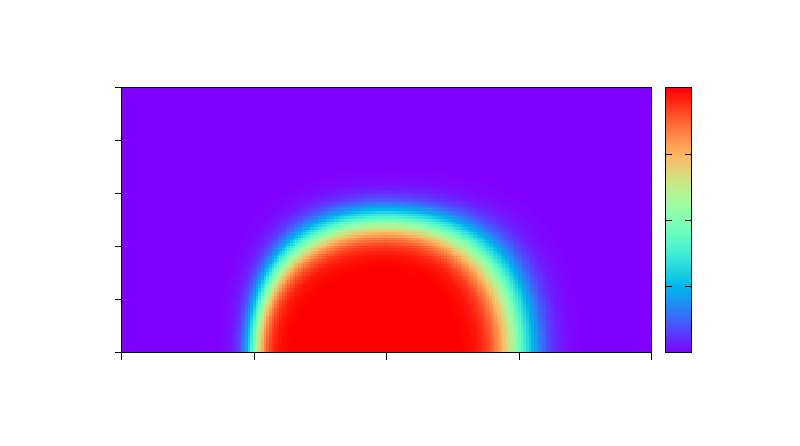
\includegraphics[width={368.50bp},height={198.40bp}]{figures/case_smith_hutton/smith_hutton_N201_Pe1.0e+04}}%
    \gplfronttext
  \end{picture}%
\endgroup
}
% 	% GNUPLOT: LaTeX picture with Postscript
\begingroup
  % Encoding inside the plot.  In the header of your document, this encoding
  % should to defined, e.g., by using
  % \usepackage[cp1252,<other encodings>]{inputenc}
  \inputencoding{cp1252}%
  \makeatletter
  \providecommand\color[2][]{%
    \GenericError{(gnuplot) \space\space\space\@spaces}{%
      Package color not loaded in conjunction with
      terminal option `colourtext'%
    }{See the gnuplot documentation for explanation.%
    }{Either use 'blacktext' in gnuplot or load the package
      color.sty in LaTeX.}%
    \renewcommand\color[2][]{}%
  }%
  \providecommand\includegraphics[2][]{%
    \GenericError{(gnuplot) \space\space\space\@spaces}{%
      Package graphicx or graphics not loaded%
    }{See the gnuplot documentation for explanation.%
    }{The gnuplot epslatex terminal needs graphicx.sty or graphics.sty.}%
    \renewcommand\includegraphics[2][]{}%
  }%
  \providecommand\rotatebox[2]{#2}%
  \@ifundefined{ifGPcolor}{%
    \newif\ifGPcolor
    \GPcolortrue
  }{}%
  \@ifundefined{ifGPblacktext}{%
    \newif\ifGPblacktext
    \GPblacktextfalse
  }{}%
  % define a \g@addto@macro without @ in the name:
  \let\gplgaddtomacro\g@addto@macro
  % define empty templates for all commands taking text:
  \gdef\gplbacktext{}%
  \gdef\gplfronttext{}%
  \makeatother
  \ifGPblacktext
    % no textcolor at all
    \def\colorrgb#1{}%
    \def\colorgray#1{}%
  \else
    % gray or color?
    \ifGPcolor
      \def\colorrgb#1{\color[rgb]{#1}}%
      \def\colorgray#1{\color[gray]{#1}}%
      \expandafter\def\csname LTw\endcsname{\color{white}}%
      \expandafter\def\csname LTb\endcsname{\color{black}}%
      \expandafter\def\csname LTa\endcsname{\color{black}}%
      \expandafter\def\csname LT0\endcsname{\color[rgb]{1,0,0}}%
      \expandafter\def\csname LT1\endcsname{\color[rgb]{0,1,0}}%
      \expandafter\def\csname LT2\endcsname{\color[rgb]{0,0,1}}%
      \expandafter\def\csname LT3\endcsname{\color[rgb]{1,0,1}}%
      \expandafter\def\csname LT4\endcsname{\color[rgb]{0,1,1}}%
      \expandafter\def\csname LT5\endcsname{\color[rgb]{1,1,0}}%
      \expandafter\def\csname LT6\endcsname{\color[rgb]{0,0,0}}%
      \expandafter\def\csname LT7\endcsname{\color[rgb]{1,0.3,0}}%
      \expandafter\def\csname LT8\endcsname{\color[rgb]{0.5,0.5,0.5}}%
    \else
      % gray
      \def\colorrgb#1{\color{black}}%
      \def\colorgray#1{\color[gray]{#1}}%
      \expandafter\def\csname LTw\endcsname{\color{white}}%
      \expandafter\def\csname LTb\endcsname{\color{black}}%
      \expandafter\def\csname LTa\endcsname{\color{black}}%
      \expandafter\def\csname LT0\endcsname{\color{black}}%
      \expandafter\def\csname LT1\endcsname{\color{black}}%
      \expandafter\def\csname LT2\endcsname{\color{black}}%
      \expandafter\def\csname LT3\endcsname{\color{black}}%
      \expandafter\def\csname LT4\endcsname{\color{black}}%
      \expandafter\def\csname LT5\endcsname{\color{black}}%
      \expandafter\def\csname LT6\endcsname{\color{black}}%
      \expandafter\def\csname LT7\endcsname{\color{black}}%
      \expandafter\def\csname LT8\endcsname{\color{black}}%
    \fi
  \fi
    \setlength{\unitlength}{0.0500bp}%
    \ifx\gptboxheight\undefined%
      \newlength{\gptboxheight}%
      \newlength{\gptboxwidth}%
      \newsavebox{\gptboxtext}%
    \fi%
    \setlength{\fboxrule}{0.5pt}%
    \setlength{\fboxsep}{1pt}%
    \definecolor{tbcol}{rgb}{1,1,1}%
\begin{picture}(7370.00,3968.00)%
    \gplgaddtomacro\gplbacktext{%
      \csname LTb\endcsname%%
      \put(814,719){\makebox(0,0)[r]{\strut{}0.0}}%
      \put(814,1234){\makebox(0,0)[r]{\strut{}0.2}}%
      \put(814,1748){\makebox(0,0)[r]{\strut{}0.4}}%
      \put(814,2263){\makebox(0,0)[r]{\strut{}0.6}}%
      \put(814,2777){\makebox(0,0)[r]{\strut{}0.8}}%
      \put(814,3292){\makebox(0,0)[r]{\strut{}1.0}}%
      \put(946,499){\makebox(0,0){\strut{}-1.0}}%
      \put(2233,499){\makebox(0,0){\strut{}-0.5}}%
      \put(3520,499){\makebox(0,0){\strut{}0.0}}%
      \put(4806,499){\makebox(0,0){\strut{}0.5}}%
      \put(6093,499){\makebox(0,0){\strut{}1.0}}%
    }%
    \gplgaddtomacro\gplfronttext{%
      \csname LTb\endcsname%%
      \put(209,2005){\rotatebox{-270}{\makebox(0,0){\strut{}$y \ (\mathrm{m})$}}}%
      \put(3519,169){\makebox(0,0){\strut{}$x \ (\mathrm{m})$}}%
      \csname LTb\endcsname%%
      \put(6611,719){\makebox(0,0)[l]{\strut{}0.0}}%
      \put(6611,1362){\makebox(0,0)[l]{\strut{}0.5}}%
      \put(6611,2005){\makebox(0,0)[l]{\strut{}1.0}}%
      \put(6611,2648){\makebox(0,0)[l]{\strut{}1.5}}%
      \put(6611,3292){\makebox(0,0)[l]{\strut{}2.0}}%
      \put(7073,2005){\rotatebox{-270}{\makebox(0,0){\strut{}$\phi$}}}%
      \put(3519,3622){\makebox(0,0){\strut{}\textbf{Smith--Hutton case} $(\mathrm{Pe} = 10^{4})$}}%
    }%
    \gplbacktext
    \put(0,0){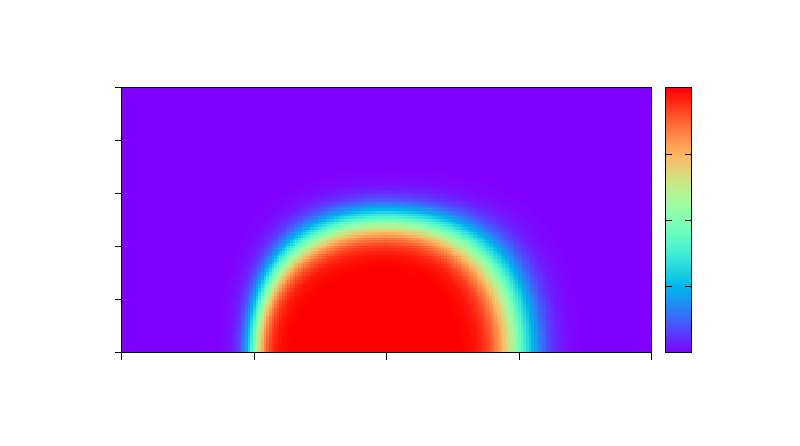
\includegraphics[width={368.50bp},height={198.40bp}]{figures/case_smith_hutton/smith_hutton_N201_Pe1.0e+04}}%
    \gplfronttext
  \end{picture}%
\endgroup

% 	\caption{Numerical solution the the Smith--Hutton case for $\rho / \Gamma = 10^4$.}
% 	\label{fig:smith_hutton_N201_Pe1.0e+04}
% \end{figure}

% \begin{figure}[ht]
% 	\centering
% 	%	\fbox{% GNUPLOT: LaTeX picture with Postscript
\documentclass{minimal}
% Set font size
\makeatletter
\def\@ptsize{1}
\InputIfFileExists{size11.clo}{}{%
   \GenericError{(gnuplot) \space\space\space\@spaces}{%
      Gnuplot Error: File `size11.clo' not found! Could not set font size%
   }{See the gnuplot documentation for explanation.%
   }{For using a font size a file `size<fontsize>.clo' has to exist.
        Falling back ^^Jto default fontsize 10pt.}%
  \def\@ptsize{0}
  \input{size10.clo}%
}%
\makeatother
% Load packages
\usepackage{calc}
\usepackage{graphicx}
\usepackage{color}
\usepackage[cp1252]{inputenc}
\makeatletter
% Select an appropriate default driver (from TeXLive graphics.cfg)
\begingroup
  \chardef\x=0 %
  % check pdfTeX
  \@ifundefined{pdfoutput}{}{%
    \ifcase\pdfoutput
    \else
      \chardef\x=1 %
    \fi
  }%
  % check VTeX
  \@ifundefined{OpMode}{}{%
    \chardef\x=2 %
  }%
\expandafter\endgroup
\ifcase\x
  % default case
  \PassOptionsToPackage{dvips}{geometry}
\or
  % pdfTeX is running in pdf mode
  \PassOptionsToPackage{pdftex}{geometry}
\else
  % VTeX is running
  \PassOptionsToPackage{vtex}{geometry}
\fi
\makeatother
% Set papersize
\usepackage[papersize={368.50bp,198.40bp},text={368.50bp,198.40bp}]{geometry}
% No page numbers and no paragraph indentation
\pagestyle{empty}
\setlength{\parindent}{0bp}%
% Load configuration file
\InputIfFileExists{gnuplot.cfg}{%
  \typeout{Using configuration file gnuplot.cfg}%
}{%
 \typeout{No configuration file gnuplot.cfg found.}%
}%
%
\begin{document}
\begingroup
  % Encoding inside the plot.  In the header of your document, this encoding
  % should to defined, e.g., by using
  % \usepackage[cp1252,<other encodings>]{inputenc}
  \inputencoding{cp1252}%
  \makeatletter
  \providecommand\color[2][]{%
    \GenericError{(gnuplot) \space\space\space\@spaces}{%
      Package color not loaded in conjunction with
      terminal option `colourtext'%
    }{See the gnuplot documentation for explanation.%
    }{Either use 'blacktext' in gnuplot or load the package
      color.sty in LaTeX.}%
    \renewcommand\color[2][]{}%
  }%
  \providecommand\includegraphics[2][]{%
    \GenericError{(gnuplot) \space\space\space\@spaces}{%
      Package graphicx or graphics not loaded%
    }{See the gnuplot documentation for explanation.%
    }{The gnuplot epslatex terminal needs graphicx.sty or graphics.sty.}%
    \renewcommand\includegraphics[2][]{}%
  }%
  \providecommand\rotatebox[2]{#2}%
  \@ifundefined{ifGPcolor}{%
    \newif\ifGPcolor
    \GPcolortrue
  }{}%
  \@ifundefined{ifGPblacktext}{%
    \newif\ifGPblacktext
    \GPblacktextfalse
  }{}%
  % define a \g@addto@macro without @ in the name:
  \let\gplgaddtomacro\g@addto@macro
  % define empty templates for all commands taking text:
  \gdef\gplbacktext{}%
  \gdef\gplfronttext{}%
  \makeatother
  \ifGPblacktext
    % no textcolor at all
    \def\colorrgb#1{}%
    \def\colorgray#1{}%
  \else
    % gray or color?
    \ifGPcolor
      \def\colorrgb#1{\color[rgb]{#1}}%
      \def\colorgray#1{\color[gray]{#1}}%
      \expandafter\def\csname LTw\endcsname{\color{white}}%
      \expandafter\def\csname LTb\endcsname{\color{black}}%
      \expandafter\def\csname LTa\endcsname{\color{black}}%
      \expandafter\def\csname LT0\endcsname{\color[rgb]{1,0,0}}%
      \expandafter\def\csname LT1\endcsname{\color[rgb]{0,1,0}}%
      \expandafter\def\csname LT2\endcsname{\color[rgb]{0,0,1}}%
      \expandafter\def\csname LT3\endcsname{\color[rgb]{1,0,1}}%
      \expandafter\def\csname LT4\endcsname{\color[rgb]{0,1,1}}%
      \expandafter\def\csname LT5\endcsname{\color[rgb]{1,1,0}}%
      \expandafter\def\csname LT6\endcsname{\color[rgb]{0,0,0}}%
      \expandafter\def\csname LT7\endcsname{\color[rgb]{1,0.3,0}}%
      \expandafter\def\csname LT8\endcsname{\color[rgb]{0.5,0.5,0.5}}%
    \else
      % gray
      \def\colorrgb#1{\color{black}}%
      \def\colorgray#1{\color[gray]{#1}}%
      \expandafter\def\csname LTw\endcsname{\color{white}}%
      \expandafter\def\csname LTb\endcsname{\color{black}}%
      \expandafter\def\csname LTa\endcsname{\color{black}}%
      \expandafter\def\csname LT0\endcsname{\color{black}}%
      \expandafter\def\csname LT1\endcsname{\color{black}}%
      \expandafter\def\csname LT2\endcsname{\color{black}}%
      \expandafter\def\csname LT3\endcsname{\color{black}}%
      \expandafter\def\csname LT4\endcsname{\color{black}}%
      \expandafter\def\csname LT5\endcsname{\color{black}}%
      \expandafter\def\csname LT6\endcsname{\color{black}}%
      \expandafter\def\csname LT7\endcsname{\color{black}}%
      \expandafter\def\csname LT8\endcsname{\color{black}}%
    \fi
  \fi
    \setlength{\unitlength}{0.0500bp}%
    \ifx\gptboxheight\undefined%
      \newlength{\gptboxheight}%
      \newlength{\gptboxwidth}%
      \newsavebox{\gptboxtext}%
    \fi%
    \setlength{\fboxrule}{0.5pt}%
    \setlength{\fboxsep}{1pt}%
    \definecolor{tbcol}{rgb}{1,1,1}%
\begin{picture}(7370.00,3968.00)%
    \gplgaddtomacro\gplbacktext{%
      \csname LTb\endcsname%%
      \put(814,733){\makebox(0,0)[r]{\strut{}0.0}}%
      \put(814,1242){\makebox(0,0)[r]{\strut{}0.2}}%
      \put(814,1751){\makebox(0,0)[r]{\strut{}0.4}}%
      \put(814,2260){\makebox(0,0)[r]{\strut{}0.6}}%
      \put(814,2769){\makebox(0,0)[r]{\strut{}0.8}}%
      \put(814,3278){\makebox(0,0)[r]{\strut{}1.0}}%
      \put(1009,513){\makebox(0,0){\strut{}-1.0}}%
      \put(2282,513){\makebox(0,0){\strut{}-0.5}}%
      \put(3554,513){\makebox(0,0){\strut{}0.0}}%
      \put(4827,513){\makebox(0,0){\strut{}0.5}}%
      \put(6099,513){\makebox(0,0){\strut{}1.0}}%
    }%
    \gplgaddtomacro\gplfronttext{%
      \csname LTb\endcsname%%
      \put(209,2005){\rotatebox{-270}{\makebox(0,0){\strut{}$y \ (\mathrm{m})$}}}%
      \put(3554,183){\makebox(0,0){\strut{}$x \ (\mathrm{m})$}}%
      \csname LTb\endcsname%%
      \put(6612,733){\makebox(0,0)[l]{\strut{}0.0}}%
      \put(6612,1369){\makebox(0,0)[l]{\strut{}0.5}}%
      \put(6612,2005){\makebox(0,0)[l]{\strut{}1.0}}%
      \put(6612,2641){\makebox(0,0)[l]{\strut{}1.5}}%
      \put(6612,3278){\makebox(0,0)[l]{\strut{}2.0}}%
      \put(7074,2005){\rotatebox{-270}{\makebox(0,0){\strut{}$\phi$}}}%
      \put(3554,3608){\makebox(0,0){\strut{}\textbf{Smith--Hutton case} $(\rho / \Gamma = 10^{6})$}}%
    }%
    \gplbacktext
    \put(0,0){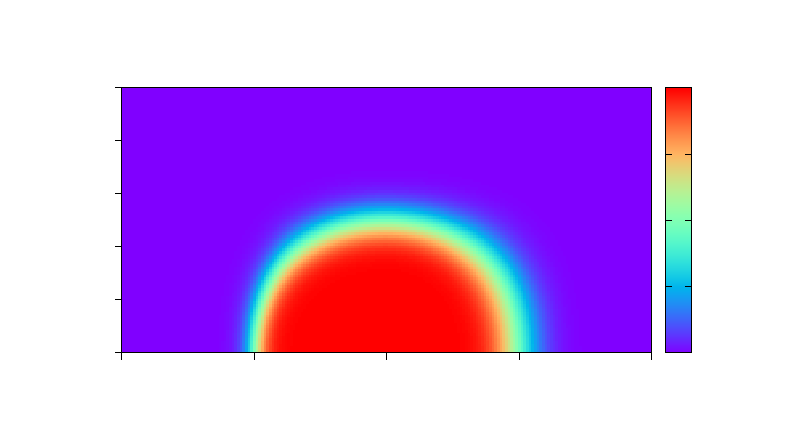
\includegraphics[width={368.50bp},height={198.40bp}]{smith_hutton_N201_Pe1.0e+06-inc}}%
    \gplfronttext
  \end{picture}%
\endgroup
\end{document}
}
% 	% GNUPLOT: LaTeX picture with Postscript
\begingroup
  % Encoding inside the plot.  In the header of your document, this encoding
  % should to defined, e.g., by using
  % \usepackage[cp1252,<other encodings>]{inputenc}
  \inputencoding{cp1252}%
  \makeatletter
  \providecommand\color[2][]{%
    \GenericError{(gnuplot) \space\space\space\@spaces}{%
      Package color not loaded in conjunction with
      terminal option `colourtext'%
    }{See the gnuplot documentation for explanation.%
    }{Either use 'blacktext' in gnuplot or load the package
      color.sty in LaTeX.}%
    \renewcommand\color[2][]{}%
  }%
  \providecommand\includegraphics[2][]{%
    \GenericError{(gnuplot) \space\space\space\@spaces}{%
      Package graphicx or graphics not loaded%
    }{See the gnuplot documentation for explanation.%
    }{The gnuplot epslatex terminal needs graphicx.sty or graphics.sty.}%
    \renewcommand\includegraphics[2][]{}%
  }%
  \providecommand\rotatebox[2]{#2}%
  \@ifundefined{ifGPcolor}{%
    \newif\ifGPcolor
    \GPcolortrue
  }{}%
  \@ifundefined{ifGPblacktext}{%
    \newif\ifGPblacktext
    \GPblacktextfalse
  }{}%
  % define a \g@addto@macro without @ in the name:
  \let\gplgaddtomacro\g@addto@macro
  % define empty templates for all commands taking text:
  \gdef\gplbacktext{}%
  \gdef\gplfronttext{}%
  \makeatother
  \ifGPblacktext
    % no textcolor at all
    \def\colorrgb#1{}%
    \def\colorgray#1{}%
  \else
    % gray or color?
    \ifGPcolor
      \def\colorrgb#1{\color[rgb]{#1}}%
      \def\colorgray#1{\color[gray]{#1}}%
      \expandafter\def\csname LTw\endcsname{\color{white}}%
      \expandafter\def\csname LTb\endcsname{\color{black}}%
      \expandafter\def\csname LTa\endcsname{\color{black}}%
      \expandafter\def\csname LT0\endcsname{\color[rgb]{1,0,0}}%
      \expandafter\def\csname LT1\endcsname{\color[rgb]{0,1,0}}%
      \expandafter\def\csname LT2\endcsname{\color[rgb]{0,0,1}}%
      \expandafter\def\csname LT3\endcsname{\color[rgb]{1,0,1}}%
      \expandafter\def\csname LT4\endcsname{\color[rgb]{0,1,1}}%
      \expandafter\def\csname LT5\endcsname{\color[rgb]{1,1,0}}%
      \expandafter\def\csname LT6\endcsname{\color[rgb]{0,0,0}}%
      \expandafter\def\csname LT7\endcsname{\color[rgb]{1,0.3,0}}%
      \expandafter\def\csname LT8\endcsname{\color[rgb]{0.5,0.5,0.5}}%
    \else
      % gray
      \def\colorrgb#1{\color{black}}%
      \def\colorgray#1{\color[gray]{#1}}%
      \expandafter\def\csname LTw\endcsname{\color{white}}%
      \expandafter\def\csname LTb\endcsname{\color{black}}%
      \expandafter\def\csname LTa\endcsname{\color{black}}%
      \expandafter\def\csname LT0\endcsname{\color{black}}%
      \expandafter\def\csname LT1\endcsname{\color{black}}%
      \expandafter\def\csname LT2\endcsname{\color{black}}%
      \expandafter\def\csname LT3\endcsname{\color{black}}%
      \expandafter\def\csname LT4\endcsname{\color{black}}%
      \expandafter\def\csname LT5\endcsname{\color{black}}%
      \expandafter\def\csname LT6\endcsname{\color{black}}%
      \expandafter\def\csname LT7\endcsname{\color{black}}%
      \expandafter\def\csname LT8\endcsname{\color{black}}%
    \fi
  \fi
    \setlength{\unitlength}{0.0500bp}%
    \ifx\gptboxheight\undefined%
      \newlength{\gptboxheight}%
      \newlength{\gptboxwidth}%
      \newsavebox{\gptboxtext}%
    \fi%
    \setlength{\fboxrule}{0.5pt}%
    \setlength{\fboxsep}{1pt}%
    \definecolor{tbcol}{rgb}{1,1,1}%
\begin{picture}(7370.00,3968.00)%
    \gplgaddtomacro\gplbacktext{%
      \csname LTb\endcsname%%
      \put(814,733){\makebox(0,0)[r]{\strut{}$0$}}%
      \put(814,1242){\makebox(0,0)[r]{\strut{}$0.2$}}%
      \put(814,1751){\makebox(0,0)[r]{\strut{}$0.4$}}%
      \put(814,2260){\makebox(0,0)[r]{\strut{}$0.6$}}%
      \put(814,2769){\makebox(0,0)[r]{\strut{}$0.8$}}%
      \put(814,3278){\makebox(0,0)[r]{\strut{}$1$}}%
      \put(1009,513){\makebox(0,0){\strut{}-1.0}}%
      \put(2282,513){\makebox(0,0){\strut{}-0.5}}%
      \put(3554,513){\makebox(0,0){\strut{}0.0}}%
      \put(4827,513){\makebox(0,0){\strut{}0.5}}%
      \put(6099,513){\makebox(0,0){\strut{}1.0}}%
    }%
    \gplgaddtomacro\gplfronttext{%
      \csname LTb\endcsname%%
      \put(209,2005){\rotatebox{-270}{\makebox(0,0){\strut{}$y \ (\mathrm{m})$}}}%
      \put(3554,183){\makebox(0,0){\strut{}$x \ (\mathrm{m})$}}%
      \csname LTb\endcsname%%
      \put(6612,733){\makebox(0,0)[l]{\strut{}0.0}}%
      \put(6612,1369){\makebox(0,0)[l]{\strut{}0.5}}%
      \put(6612,2005){\makebox(0,0)[l]{\strut{}1.0}}%
      \put(6612,2641){\makebox(0,0)[l]{\strut{}1.5}}%
      \put(6612,3278){\makebox(0,0)[l]{\strut{}2.0}}%
      \put(7074,2005){\rotatebox{-270}{\makebox(0,0){\strut{}$\phi$}}}%
      \put(3554,3608){\makebox(0,0){\strut{}\textbf{Smith--Hutton case} $(\rho / \Gamma = 10^{9})$}}%
    }%
    \gplbacktext
    \put(0,0){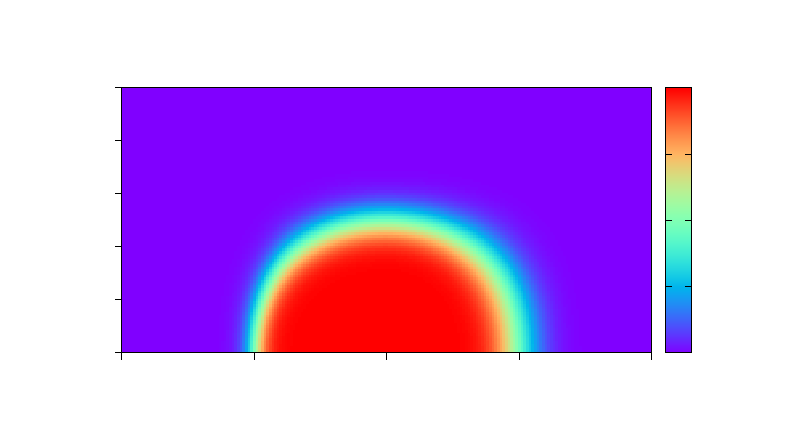
\includegraphics[width={368.50bp},height={198.40bp}]{figures/case_smith_hutton/smith_hutton_N201_Pe1.0e+09}}%
    \gplfronttext
  \end{picture}%
\endgroup

% 	\caption{Numerical solution the the Smith--Hutton case for $\rho / \Gamma = 10^9$.}
% 	\label{fig:smith_hutton_N201_Pe1.0e+09}
% \end{figure}

% /////////////////////////////////////////////////////////////////////////////////////

\clearpage

Figures \ref{fig:smith_hutton_N201_Pe1.0e-01} and
\ref{fig:smith_hutton_N201_Pe1.0e-09} show the solution to the Smith--Hutton
case for $\rho / \Gamma = 10^{-1}$ and $\rho / \Gamma = 10^{-9}$, respectively.
Although a quotient $\rho / \Gamma = 10^{-9}$ implies transport is much weaker
than for $\rho / \Gamma = 10^{-1}$, the differences between both solution are
difficult to detect. The only apparent discrepancy is the central zone of
$\Omega$, where the transitions for $\rho / \Gamma = 10^{-9}$ are much smoother
than for $\rho / \Gamma = 10^{-1}$, which implies transport has lost strength.

\begin{figure}[ht]
	\centering
	%	\fbox{% GNUPLOT: LaTeX picture with Postscript
\begingroup
  % Encoding inside the plot.  In the header of your document, this encoding
  % should to defined, e.g., by using
  % \usepackage[cp1252,<other encodings>]{inputenc}
  \inputencoding{cp1252}%
  \makeatletter
  \providecommand\color[2][]{%
    \GenericError{(gnuplot) \space\space\space\@spaces}{%
      Package color not loaded in conjunction with
      terminal option `colourtext'%
    }{See the gnuplot documentation for explanation.%
    }{Either use 'blacktext' in gnuplot or load the package
      color.sty in LaTeX.}%
    \renewcommand\color[2][]{}%
  }%
  \providecommand\includegraphics[2][]{%
    \GenericError{(gnuplot) \space\space\space\@spaces}{%
      Package graphicx or graphics not loaded%
    }{See the gnuplot documentation for explanation.%
    }{The gnuplot epslatex terminal needs graphicx.sty or graphics.sty.}%
    \renewcommand\includegraphics[2][]{}%
  }%
  \providecommand\rotatebox[2]{#2}%
  \@ifundefined{ifGPcolor}{%
    \newif\ifGPcolor
    \GPcolortrue
  }{}%
  \@ifundefined{ifGPblacktext}{%
    \newif\ifGPblacktext
    \GPblacktextfalse
  }{}%
  % define a \g@addto@macro without @ in the name:
  \let\gplgaddtomacro\g@addto@macro
  % define empty templates for all commands taking text:
  \gdef\gplbacktext{}%
  \gdef\gplfronttext{}%
  \makeatother
  \ifGPblacktext
    % no textcolor at all
    \def\colorrgb#1{}%
    \def\colorgray#1{}%
  \else
    % gray or color?
    \ifGPcolor
      \def\colorrgb#1{\color[rgb]{#1}}%
      \def\colorgray#1{\color[gray]{#1}}%
      \expandafter\def\csname LTw\endcsname{\color{white}}%
      \expandafter\def\csname LTb\endcsname{\color{black}}%
      \expandafter\def\csname LTa\endcsname{\color{black}}%
      \expandafter\def\csname LT0\endcsname{\color[rgb]{1,0,0}}%
      \expandafter\def\csname LT1\endcsname{\color[rgb]{0,1,0}}%
      \expandafter\def\csname LT2\endcsname{\color[rgb]{0,0,1}}%
      \expandafter\def\csname LT3\endcsname{\color[rgb]{1,0,1}}%
      \expandafter\def\csname LT4\endcsname{\color[rgb]{0,1,1}}%
      \expandafter\def\csname LT5\endcsname{\color[rgb]{1,1,0}}%
      \expandafter\def\csname LT6\endcsname{\color[rgb]{0,0,0}}%
      \expandafter\def\csname LT7\endcsname{\color[rgb]{1,0.3,0}}%
      \expandafter\def\csname LT8\endcsname{\color[rgb]{0.5,0.5,0.5}}%
    \else
      % gray
      \def\colorrgb#1{\color{black}}%
      \def\colorgray#1{\color[gray]{#1}}%
      \expandafter\def\csname LTw\endcsname{\color{white}}%
      \expandafter\def\csname LTb\endcsname{\color{black}}%
      \expandafter\def\csname LTa\endcsname{\color{black}}%
      \expandafter\def\csname LT0\endcsname{\color{black}}%
      \expandafter\def\csname LT1\endcsname{\color{black}}%
      \expandafter\def\csname LT2\endcsname{\color{black}}%
      \expandafter\def\csname LT3\endcsname{\color{black}}%
      \expandafter\def\csname LT4\endcsname{\color{black}}%
      \expandafter\def\csname LT5\endcsname{\color{black}}%
      \expandafter\def\csname LT6\endcsname{\color{black}}%
      \expandafter\def\csname LT7\endcsname{\color{black}}%
      \expandafter\def\csname LT8\endcsname{\color{black}}%
    \fi
  \fi
    \setlength{\unitlength}{0.0500bp}%
    \ifx\gptboxheight\undefined%
      \newlength{\gptboxheight}%
      \newlength{\gptboxwidth}%
      \newsavebox{\gptboxtext}%
    \fi%
    \setlength{\fboxrule}{0.5pt}%
    \setlength{\fboxsep}{1pt}%
    \definecolor{tbcol}{rgb}{1,1,1}%
\begin{picture}(7370.00,3968.00)%
    \gplgaddtomacro\gplbacktext{%
      \csname LTb\endcsname%%
      \put(814,719){\makebox(0,0)[r]{\strut{}0.0}}%
      \put(814,1234){\makebox(0,0)[r]{\strut{}0.2}}%
      \put(814,1748){\makebox(0,0)[r]{\strut{}0.4}}%
      \put(814,2263){\makebox(0,0)[r]{\strut{}0.6}}%
      \put(814,2777){\makebox(0,0)[r]{\strut{}0.8}}%
      \put(814,3292){\makebox(0,0)[r]{\strut{}1.0}}%
      \put(946,499){\makebox(0,0){\strut{}-1.0}}%
      \put(2233,499){\makebox(0,0){\strut{}-0.5}}%
      \put(3520,499){\makebox(0,0){\strut{}0.0}}%
      \put(4806,499){\makebox(0,0){\strut{}0.5}}%
      \put(6093,499){\makebox(0,0){\strut{}1.0}}%
    }%
    \gplgaddtomacro\gplfronttext{%
      \csname LTb\endcsname%%
      \put(209,2005){\rotatebox{-270}{\makebox(0,0){\strut{}$y \ (\mathrm{m})$}}}%
      \put(3519,169){\makebox(0,0){\strut{}$x \ (\mathrm{m})$}}%
      \csname LTb\endcsname%%
      \put(6611,719){\makebox(0,0)[l]{\strut{}0.0}}%
      \put(6611,1362){\makebox(0,0)[l]{\strut{}0.5}}%
      \put(6611,2005){\makebox(0,0)[l]{\strut{}1.0}}%
      \put(6611,2648){\makebox(0,0)[l]{\strut{}1.5}}%
      \put(6611,3292){\makebox(0,0)[l]{\strut{}2.0}}%
      \put(7073,2005){\rotatebox{-270}{\makebox(0,0){\strut{}$\phi$}}}%
      \put(3519,3622){\makebox(0,0){\strut{}\textbf{Smith--Hutton case} $(\mathrm{Pe} = 10^{-1})$}}%
    }%
    \gplbacktext
    \put(0,0){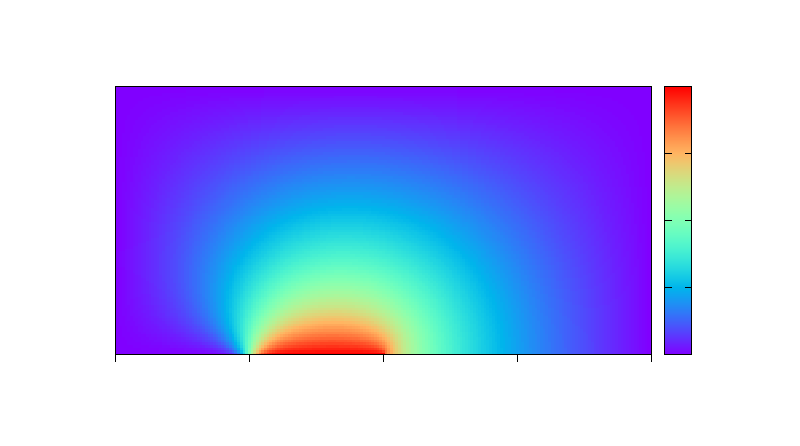
\includegraphics[width={368.50bp},height={198.40bp}]{figures/case_smith_hutton/smith_hutton_N201_Pe1.0e-01}}%
    \gplfronttext
  \end{picture}%
\endgroup
}
	% GNUPLOT: LaTeX picture with Postscript
\begingroup
  % Encoding inside the plot.  In the header of your document, this encoding
  % should to defined, e.g., by using
  % \usepackage[cp1252,<other encodings>]{inputenc}
  \inputencoding{cp1252}%
  \makeatletter
  \providecommand\color[2][]{%
    \GenericError{(gnuplot) \space\space\space\@spaces}{%
      Package color not loaded in conjunction with
      terminal option `colourtext'%
    }{See the gnuplot documentation for explanation.%
    }{Either use 'blacktext' in gnuplot or load the package
      color.sty in LaTeX.}%
    \renewcommand\color[2][]{}%
  }%
  \providecommand\includegraphics[2][]{%
    \GenericError{(gnuplot) \space\space\space\@spaces}{%
      Package graphicx or graphics not loaded%
    }{See the gnuplot documentation for explanation.%
    }{The gnuplot epslatex terminal needs graphicx.sty or graphics.sty.}%
    \renewcommand\includegraphics[2][]{}%
  }%
  \providecommand\rotatebox[2]{#2}%
  \@ifundefined{ifGPcolor}{%
    \newif\ifGPcolor
    \GPcolortrue
  }{}%
  \@ifundefined{ifGPblacktext}{%
    \newif\ifGPblacktext
    \GPblacktextfalse
  }{}%
  % define a \g@addto@macro without @ in the name:
  \let\gplgaddtomacro\g@addto@macro
  % define empty templates for all commands taking text:
  \gdef\gplbacktext{}%
  \gdef\gplfronttext{}%
  \makeatother
  \ifGPblacktext
    % no textcolor at all
    \def\colorrgb#1{}%
    \def\colorgray#1{}%
  \else
    % gray or color?
    \ifGPcolor
      \def\colorrgb#1{\color[rgb]{#1}}%
      \def\colorgray#1{\color[gray]{#1}}%
      \expandafter\def\csname LTw\endcsname{\color{white}}%
      \expandafter\def\csname LTb\endcsname{\color{black}}%
      \expandafter\def\csname LTa\endcsname{\color{black}}%
      \expandafter\def\csname LT0\endcsname{\color[rgb]{1,0,0}}%
      \expandafter\def\csname LT1\endcsname{\color[rgb]{0,1,0}}%
      \expandafter\def\csname LT2\endcsname{\color[rgb]{0,0,1}}%
      \expandafter\def\csname LT3\endcsname{\color[rgb]{1,0,1}}%
      \expandafter\def\csname LT4\endcsname{\color[rgb]{0,1,1}}%
      \expandafter\def\csname LT5\endcsname{\color[rgb]{1,1,0}}%
      \expandafter\def\csname LT6\endcsname{\color[rgb]{0,0,0}}%
      \expandafter\def\csname LT7\endcsname{\color[rgb]{1,0.3,0}}%
      \expandafter\def\csname LT8\endcsname{\color[rgb]{0.5,0.5,0.5}}%
    \else
      % gray
      \def\colorrgb#1{\color{black}}%
      \def\colorgray#1{\color[gray]{#1}}%
      \expandafter\def\csname LTw\endcsname{\color{white}}%
      \expandafter\def\csname LTb\endcsname{\color{black}}%
      \expandafter\def\csname LTa\endcsname{\color{black}}%
      \expandafter\def\csname LT0\endcsname{\color{black}}%
      \expandafter\def\csname LT1\endcsname{\color{black}}%
      \expandafter\def\csname LT2\endcsname{\color{black}}%
      \expandafter\def\csname LT3\endcsname{\color{black}}%
      \expandafter\def\csname LT4\endcsname{\color{black}}%
      \expandafter\def\csname LT5\endcsname{\color{black}}%
      \expandafter\def\csname LT6\endcsname{\color{black}}%
      \expandafter\def\csname LT7\endcsname{\color{black}}%
      \expandafter\def\csname LT8\endcsname{\color{black}}%
    \fi
  \fi
    \setlength{\unitlength}{0.0500bp}%
    \ifx\gptboxheight\undefined%
      \newlength{\gptboxheight}%
      \newlength{\gptboxwidth}%
      \newsavebox{\gptboxtext}%
    \fi%
    \setlength{\fboxrule}{0.5pt}%
    \setlength{\fboxsep}{1pt}%
    \definecolor{tbcol}{rgb}{1,1,1}%
\begin{picture}(7370.00,3968.00)%
    \gplgaddtomacro\gplbacktext{%
      \csname LTb\endcsname%%
      \put(814,719){\makebox(0,0)[r]{\strut{}0.0}}%
      \put(814,1234){\makebox(0,0)[r]{\strut{}0.2}}%
      \put(814,1748){\makebox(0,0)[r]{\strut{}0.4}}%
      \put(814,2263){\makebox(0,0)[r]{\strut{}0.6}}%
      \put(814,2777){\makebox(0,0)[r]{\strut{}0.8}}%
      \put(814,3292){\makebox(0,0)[r]{\strut{}1.0}}%
      \put(946,499){\makebox(0,0){\strut{}-1.0}}%
      \put(2233,499){\makebox(0,0){\strut{}-0.5}}%
      \put(3520,499){\makebox(0,0){\strut{}0.0}}%
      \put(4806,499){\makebox(0,0){\strut{}0.5}}%
      \put(6093,499){\makebox(0,0){\strut{}1.0}}%
    }%
    \gplgaddtomacro\gplfronttext{%
      \csname LTb\endcsname%%
      \put(209,2005){\rotatebox{-270}{\makebox(0,0){\strut{}$y \ (\mathrm{m})$}}}%
      \put(3519,169){\makebox(0,0){\strut{}$x \ (\mathrm{m})$}}%
      \csname LTb\endcsname%%
      \put(6611,719){\makebox(0,0)[l]{\strut{}0.0}}%
      \put(6611,1362){\makebox(0,0)[l]{\strut{}0.5}}%
      \put(6611,2005){\makebox(0,0)[l]{\strut{}1.0}}%
      \put(6611,2648){\makebox(0,0)[l]{\strut{}1.5}}%
      \put(6611,3292){\makebox(0,0)[l]{\strut{}2.0}}%
      \put(7073,2005){\rotatebox{-270}{\makebox(0,0){\strut{}$\phi$}}}%
      \put(3519,3622){\makebox(0,0){\strut{}\textbf{Smith--Hutton case} $(\mathrm{Pe} = 10^{-1})$}}%
    }%
    \gplbacktext
    \put(0,0){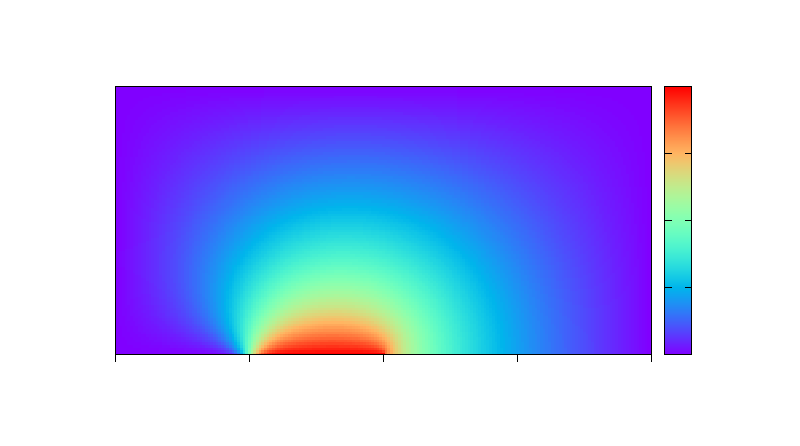
\includegraphics[width={368.50bp},height={198.40bp}]{figures/case_smith_hutton/smith_hutton_N201_Pe1.0e-01}}%
    \gplfronttext
  \end{picture}%
\endgroup

	\caption{Numerical solution the the Smith--Hutton case for $\rho / \Gamma = 10^{-1}$.}
	\label{fig:smith_hutton_N201_Pe1.0e-01}
	\vspace{1cm}
	% GNUPLOT: LaTeX picture with Postscript
\begingroup
  % Encoding inside the plot.  In the header of your document, this encoding
  % should to defined, e.g., by using
  % \usepackage[cp1252,<other encodings>]{inputenc}
  \inputencoding{cp1252}%
  \makeatletter
  \providecommand\color[2][]{%
    \GenericError{(gnuplot) \space\space\space\@spaces}{%
      Package color not loaded in conjunction with
      terminal option `colourtext'%
    }{See the gnuplot documentation for explanation.%
    }{Either use 'blacktext' in gnuplot or load the package
      color.sty in LaTeX.}%
    \renewcommand\color[2][]{}%
  }%
  \providecommand\includegraphics[2][]{%
    \GenericError{(gnuplot) \space\space\space\@spaces}{%
      Package graphicx or graphics not loaded%
    }{See the gnuplot documentation for explanation.%
    }{The gnuplot epslatex terminal needs graphicx.sty or graphics.sty.}%
    \renewcommand\includegraphics[2][]{}%
  }%
  \providecommand\rotatebox[2]{#2}%
  \@ifundefined{ifGPcolor}{%
    \newif\ifGPcolor
    \GPcolortrue
  }{}%
  \@ifundefined{ifGPblacktext}{%
    \newif\ifGPblacktext
    \GPblacktextfalse
  }{}%
  % define a \g@addto@macro without @ in the name:
  \let\gplgaddtomacro\g@addto@macro
  % define empty templates for all commands taking text:
  \gdef\gplbacktext{}%
  \gdef\gplfronttext{}%
  \makeatother
  \ifGPblacktext
    % no textcolor at all
    \def\colorrgb#1{}%
    \def\colorgray#1{}%
  \else
    % gray or color?
    \ifGPcolor
      \def\colorrgb#1{\color[rgb]{#1}}%
      \def\colorgray#1{\color[gray]{#1}}%
      \expandafter\def\csname LTw\endcsname{\color{white}}%
      \expandafter\def\csname LTb\endcsname{\color{black}}%
      \expandafter\def\csname LTa\endcsname{\color{black}}%
      \expandafter\def\csname LT0\endcsname{\color[rgb]{1,0,0}}%
      \expandafter\def\csname LT1\endcsname{\color[rgb]{0,1,0}}%
      \expandafter\def\csname LT2\endcsname{\color[rgb]{0,0,1}}%
      \expandafter\def\csname LT3\endcsname{\color[rgb]{1,0,1}}%
      \expandafter\def\csname LT4\endcsname{\color[rgb]{0,1,1}}%
      \expandafter\def\csname LT5\endcsname{\color[rgb]{1,1,0}}%
      \expandafter\def\csname LT6\endcsname{\color[rgb]{0,0,0}}%
      \expandafter\def\csname LT7\endcsname{\color[rgb]{1,0.3,0}}%
      \expandafter\def\csname LT8\endcsname{\color[rgb]{0.5,0.5,0.5}}%
    \else
      % gray
      \def\colorrgb#1{\color{black}}%
      \def\colorgray#1{\color[gray]{#1}}%
      \expandafter\def\csname LTw\endcsname{\color{white}}%
      \expandafter\def\csname LTb\endcsname{\color{black}}%
      \expandafter\def\csname LTa\endcsname{\color{black}}%
      \expandafter\def\csname LT0\endcsname{\color{black}}%
      \expandafter\def\csname LT1\endcsname{\color{black}}%
      \expandafter\def\csname LT2\endcsname{\color{black}}%
      \expandafter\def\csname LT3\endcsname{\color{black}}%
      \expandafter\def\csname LT4\endcsname{\color{black}}%
      \expandafter\def\csname LT5\endcsname{\color{black}}%
      \expandafter\def\csname LT6\endcsname{\color{black}}%
      \expandafter\def\csname LT7\endcsname{\color{black}}%
      \expandafter\def\csname LT8\endcsname{\color{black}}%
    \fi
  \fi
    \setlength{\unitlength}{0.0500bp}%
    \ifx\gptboxheight\undefined%
      \newlength{\gptboxheight}%
      \newlength{\gptboxwidth}%
      \newsavebox{\gptboxtext}%
    \fi%
    \setlength{\fboxrule}{0.5pt}%
    \setlength{\fboxsep}{1pt}%
    \definecolor{tbcol}{rgb}{1,1,1}%
\begin{picture}(7370.00,3968.00)%
    \gplgaddtomacro\gplbacktext{%
      \csname LTb\endcsname%%
      \put(814,733){\makebox(0,0)[r]{\strut{}$0$}}%
      \put(814,1242){\makebox(0,0)[r]{\strut{}$0.2$}}%
      \put(814,1751){\makebox(0,0)[r]{\strut{}$0.4$}}%
      \put(814,2260){\makebox(0,0)[r]{\strut{}$0.6$}}%
      \put(814,2769){\makebox(0,0)[r]{\strut{}$0.8$}}%
      \put(814,3278){\makebox(0,0)[r]{\strut{}$1$}}%
      \put(1009,513){\makebox(0,0){\strut{}-1.0}}%
      \put(2282,513){\makebox(0,0){\strut{}-0.5}}%
      \put(3554,513){\makebox(0,0){\strut{}0.0}}%
      \put(4827,513){\makebox(0,0){\strut{}0.5}}%
      \put(6099,513){\makebox(0,0){\strut{}1.0}}%
    }%
    \gplgaddtomacro\gplfronttext{%
      \csname LTb\endcsname%%
      \put(209,2005){\rotatebox{-270}{\makebox(0,0){\strut{}$y \ (\mathrm{m})$}}}%
      \put(3554,183){\makebox(0,0){\strut{}$x \ (\mathrm{m})$}}%
      \csname LTb\endcsname%%
      \put(6612,733){\makebox(0,0)[l]{\strut{}0.0}}%
      \put(6612,1369){\makebox(0,0)[l]{\strut{}0.5}}%
      \put(6612,2005){\makebox(0,0)[l]{\strut{}1.0}}%
      \put(6612,2641){\makebox(0,0)[l]{\strut{}1.5}}%
      \put(6612,3278){\makebox(0,0)[l]{\strut{}2.0}}%
      \put(7074,2005){\rotatebox{-270}{\makebox(0,0){\strut{}$\phi$}}}%
      \put(3554,3608){\makebox(0,0){\strut{}\textbf{Smith--Hutton case} $(\rho / \Gamma = 10^{-9})$}}%
    }%
    \gplbacktext
    \put(0,0){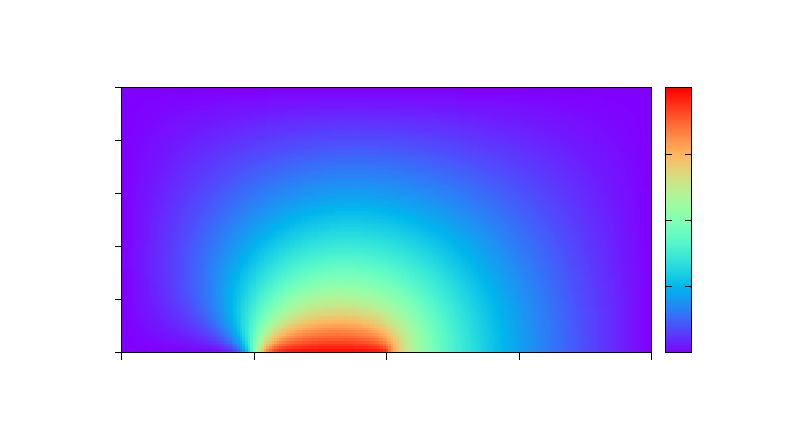
\includegraphics[width={368.50bp},height={198.40bp}]{figures/case_smith_hutton/smith_hutton_N201_Pe1.0e-09}}%
    \gplfronttext
  \end{picture}%
\endgroup

	\caption{Numerical solution the the Smith--Hutton case for $\rho / \Gamma = 10^{-9}$.}
	\label{fig:smith_hutton_N201_Pe1.0e-09}
\end{figure}








\begin{figure}[h]
	\centering
	\begin{tikzpicture}
		\def\lx{6}
		\def\ly{4}
		\def\nx{7}
		\def\ny{5}
		\def\stepx{\lx/(\nx-1)}
		\def\stepy{\ly/(\ny-1)}
		\draw[very thick] (0,0) rectangle (\lx,\ly);
		% Nodes
		\foreach \x in {0,...,6}
			\foreach \y in {0,...,4}
				\filldraw[blue] ({\x*\stepx},{\y*\stepy}) circle (2pt);
		% Control volumes
		\foreach \x in {1,...,6}
			\draw[thick, dashed] ({-0.5*\stepx+\x*\stepx},0) -- ++(0,\ly);
		\foreach \y in {1,...,4}
			\draw[thick, dashed] (0,{-0.5*\stepy+\y*\stepy}) -- ++(\lx,0);
	\end{tikzpicture}
\end{figure}

\clearpage 	\printbibliography

\clearpage 
\appendix


\section{Some results on Measure Theory} \label{ap:measure_theory}

In this appendix we gather two important theorems needed to justify some steps
in the derivation of conservation laws in section
\ref{sec:the_convection_diffusion_equations}. Despite these results are basic, a
previous study of real analysis is required in order to understand and prove
them. A good reference for the interested reader is Real and Complex Analysis of
Walter Rudin \cite{rudin1987real}. 

\subsection{Differentiation under the integral sign}

Differentiation under the integral sign allows us to compute the derivative of
an integral of a function of two parameters in a simple way. It is needed, for
instance, when the mass conservation law or the heat diffusion equation are
derived. 

Let $(X, \mathcal{A}, \mu)$ be a measure space and let $[a, b] \subset \real$.
Hereinafter we deal with functions $f \colon X \times [a,b] \rightarrow \real$,
where $t \in [a, b]$ is the parameter on which $f$ depends. We assume that
$f(\cdot, t)$ is a measurable function for each $t \in [a, b]$.

\begin{theorem}[Differentiation under the integral sign]
	\label{theo:differentiation_under_the_integral_sign} Let $F(t) = \int_X
	f(x,t) \dd{\mu}$. Assume that
	\begin{enumerate}[label={(\roman*)}, topsep=0pt]
		\item $f(x,t_0)$ is an integrable function for some $t_0 \in
		[a,b]$.
		\item $\dfrac{\partial f}{\partial t}(x,t)$ is defined for all
		$(x, t) \in X \times [a, b]$.
		\item There exists an integral function $g \colon X \rightarrow \real$
		such that $\abs{\dfrac{\partial f}{\partial t} (x,t)} \leq
		g(x)$ for all $(x, t) \in X \times [a, b]$.
	\end{enumerate}
	Then $F$ is a differentiable function and
	\[
		F'(t) = \frac{\dd}{\dd t} F(t) = \int_X \frac{\partial f}{\partial t}(x,t) \dd{\mu}
	\]
\end{theorem}

For the applications needed in this project, $X = \real^m$ with $1 \leq m \leq
3$, $\mathcal{A}$ is the Borel $\sigma$--algebra on $\real^m$ and $\mu$ is
Lebesgue's measure on $\real^m$, which for most of the ``natural'' sets of
$\mathcal{A}$ coincides with the usual notion of $m$--dimensional volume.

\subsection{Lebesgue's differentiation lemma}

A common way to derive a conservation law is to integrate some functions in a
control volume, then apply Differentiation under the integral sign to obtain an
integral equation and finally get to a differential equation using Lebesgue's
differentiation lemma. 

An intuitive way to understand and to motivate Lebesgue's differentiation lemma
is the following. Let $f \colon \real \to \real$ be a continuous function, let
$a \in \real$ be a fixed point and let $F(x) = \int_a^x f(y) \dd{y}$, which is a
differentiable function. Due to a corollary of the Fundamental Theorem of
Calculus, we have $F'(x) = f(x)$. Using the definition of derivative,
\[
	F'(x) = 
	\lim_{h \to 0} \frac{F(x + h) - F(x)}{h} = 
	\lim_{h \to 0} \frac{1}{h} \left\{ \int_a^{x + h} f(y) \dd{y} - \int_a^{x} f(y) \dd{y} \right\} = 
	\lim_{h \to 0} \frac{1}{h} \int_x^{x + h} f(y) \dd{y} = f(x)
\]
Notice that the integral is divided by the length of the interval $[x, x+h]$,
otherwise the limit would be zero. Lebesgue's lemma generalizes the previous
equality by considering functions $f \colon \real^n \to \real$ and integrating
them on open balls $B(x_0, r) = \{ x \in \real^n \mid \norm{x -
x_0} < r\}$. Furthermore, the integral is divided by the $n$--dimensional
volume of $B(x_0, r)$, which is denoted by $\abs{B(x_0, r)}$.

\begin{theorem}[Lebesgue's differentiation lemma \cite{evans1998pde}]
	\label{eq:lebesgue_differentiation_lemma} Let $f \colon \real^n \rightarrow
	\real$ be a locally integrable function.
	\begin{enumerate}[label={(\arabic*)}, topsep=0pt]
		\item Then for almost everywhere point $x_0 \in \real^n$,
		\[
			\frac{1}{\abs{B(x_0, r)}} \int_{B(x_0,r)} f(x) \dd{x} \to f(x_0) 
			\quad \text{as } r \to 0
		\]
		\item In fact, for almost everywhere point $x_0 \in \real^n$,
		\[
			\frac{1}{\abs{B(x_0, r)}} \int_{B(x_0,r)} \abs{f(x) - f(x_0)} \dd{x} \to 0 
			\quad \text{as } r \to 0
		\]		
	\end{enumerate}
\end{theorem}


\section{Ordinary Differential Equations}

In this appendix we present a central theorem in basic Ordinary differential
equations (ODE) theory regarding the existence and uniqueness of solution to
initial value problems involving ODEs. Later this theorem is particularized to
the case of linear ODEs. Finally it is shown that any linear ODE of order $n$
can be rewritten as a linear system of ODEs.

Recall that an ordinary differential equation is an equation
\begin{equation*}
	g(t, x(t), x'(t), \ldots, x^{(n)}(t)) = 0
\end{equation*}
where the unknown $x(t) = (x_1(t), \ldots, x_m(t))^\top$ is a function of $m$
components and a variable $t \in \real$, $x' = \dfrac{\dd{x}}{\dd{t}}$ and $g(t,
y_1, \ldots, y_{n+1})$ with $y_1, \ldots, y_{n+1} \in \real^m$ is a function of
$1 + m(n+1)$ variables.

\subsection{General theory}

We begin with the definition of a Lipschitz function:

\begin{definition*}
	A function $f \colon \Omega \subset \real^n \rightarrow \real^m$ is said to
	be Lipschitz or Lipschitz continuous if there exists a constant $L$ such
	that
	\begin{equation*}
		\norm{f(x) - f(y)} \leq L \norm{x - y}
	\end{equation*}
	for every $x, y \in \Omega$. The constant $L$ is called the
	Lipschitz constant of $f$ \cite{salsa2009pde}.
\end{definition*}

Every Lipschitz function on $\Omega$ is also a continuous function in the usual
sense on $\Omega$. The converse is not true in general, and depends on $\Omega$.
The Lipschitz continuity is actually a very restrictive condition, since it
imposes that the function can grow at most as a linear function. 

\begin{definition*}
	Let $(E, \norm{\cdot}_E)$ and $(F, \norm{\cdot}_F)$ be two finite
	dimensional normed vector spaces and let $A \colon E \rightarrow F$ be a
	linear mapping between them. The norm of $A$ is defined to be
	\begin{equation*}
		\norm{A} \coloneqq 
		\sup{\left\{ \norm{A x}_F \mid x \in E, \ \norm{x}_E \leq 1 \right\}}
	\end{equation*}
\end{definition*}

\noindent
It is a well known fact that $\norm{A}$ is finite. In some cases, proving that a
function is Lipschitz continuous is a laborious task. In these situations we
have the following theorems:

\begin{theorem}[Corollary of the mean value theorem \cite{mazon2008calculo}]
	\label{teo:corollary_mean_value_theorem} Let $\Omega \subset \real^n$ an
	open set and let $f \colon \Omega \subset \real^n \to \real^m$ a
	differentiable function on $\Omega$. Let $x, y \in \Omega$ such
	that the segment $\overline{xy} = \{ \lambda x + (1 -
	\lambda) y \mid \lambda \in [0, 1] \}$ is contained in $\Omega$. Then
	the following inequality holds:
	\begin{equation*}
		\norm{f(x) - f(y)} \leq \sup_{z \in 
		\overline{xy}} \norm{D f(z)} \norm{x - y}
	\end{equation*}
\end{theorem}
\begin{proof}
	See \cite{mazon2008calculo}, page 78.
\end{proof}

\begin{theorem} \label{teo:c1_function_implies_lipschitz} Let $\Omega \subset
	\real^n$ a compact convex set and let $f \equiv (f_1, \ldots, f_m) \colon
	\Omega \subset \real^n \to \real^m$ a $\mathcal{C}^1(\Omega)$ function. Then
	$f$ is Lipschitz in $\Omega$.
\end{theorem}
\begin{proof}
	The differential of $D f$, given by
	\begin{equation*}
		D f = 
		\begin{pmatrix}
			\pdv{f_1}{x_1} & \cdots & \pdv{f_1}{x_n} \\[6pt]
			\vdots & \ddots & \vdots \\[6pt]
			\pdv{f_m}{x_1} & \cdots & \pdv{f_m}{x_n} \\
		\end{pmatrix}
	\end{equation*}
	is a linear mapping $D f \colon \real^n \rightarrow \real^m$. Since $f$ is
	$\mathcal{C}^1(\Omega)$ function, the partial derivatives $\pdv{f_1}{x_1},
	\ldots, \pdv{f_m}{x_n}$ are continuous functions on $\Omega$. Moreover, the
	norm of the differential depends continuously on the partial derivatives
	$\pdv{f_1}{x_1}, \ldots, \pdv{f_m}{x_n}$ and on $z$. As a consequence,
	$\norm{D f}$ is a continuous function on $\Omega$. By Weierstrass theorem,
	$\norm{D f}$ reaches a maximum $M$ on $\Omega$. Applying theorem
	\ref{teo:corollary_mean_value_theorem} we have 
	\begin{equation*}
		\norm{f(x) - f(y)} \leq \sup_{z \in 
		\overline{xy}} \norm{D f(z)} \norm{x - y} \leq
		M \norm{x - y}
	\end{equation*}
	for all $x, y \in \Omega$, hence $f$ is Lipschitz on
	$\overline{\Omega}$.
\end{proof}

Finally we can state the Picard--Lindelöf theorem. Let $U$ be an open subset of
$\real^{n+1}$ and let $f \in C(U, \real)$, $(t_0, x_0) \in U$. Consider the
following IVP:
\begin{equation} \label{eq:appendix_ode_ivp}
	\left\{
	\begin{aligned}
		&\dot{x}(t) = f(t, x) \\
		&x(t_0) = x_0
	\end{aligned}
	\right.
\end{equation}
The Picard--Lindelöf theorem gives us the existence and uniqueness of solution
for \eqref{eq:appendix_ode_ivp}.

\begin{theorem}[Picard--Lindelöf \cite{teschl2012odes}]
	\label{teo:picard_lindelof} Suppose $f \in \mathcal{C}(U, \real^n)$, where
	$U$ is an open subset of $\real^{n+1}$, and $(t_0, x_0) \in U$. If $f$
	is locally Lipschitz continuous in the second argument, uniformly with
	respect to the first, then there exists a unique local solution $x(t)
	\in \mathcal{C}^1(I)$ of the initial value problem
	\eqref{eq:appendix_ode_ivp}, where $I$ is some interval around $t_0$. 
	
	More specifically, if $V = [t_0, t_0 + T] \times \overline{B(x_0,
	\delta)} \subset U$ and $M$ denotes the maximum of $\abs{f}$ on $V$, then
	the solution exists at least for $t \in [t_0, t_0 + T_0]$ and remains in
	$\overline{B(x_0, \delta)}$ where $T_0 = \min{\left\{ T,
	\frac{\delta}{M} \right\}}$. The analogous result holds for the interval
	$[t_0 - T, t_0]$.
\end{theorem}
\begin{proof}
	See \cite{teschl2012odes}, page 38.
\end{proof}


\subsection{Linear equations}

Let $\mathcal{M}_{n \times n}(\real)$ and $\mathcal{M}_{n \times n}(\cplex)$
denote the space of $n \times n$ matrices with real or complex coefficients,
respectively. Recall that an ODE or a system of ODEs is linear if it has the
form
\begin{equation} \label{eq:linear_ode}
	\dot{x} = A(t) x + b(t)
\end{equation}
where $A(t) \in \mathcal{M}_{n \times n}(\real)$ (or $A(t) \in \mathcal{M}_{n
\times n}(\cplex)$) and $b(t) \in \real^n$ for all $t \in I \subset \real$. The
following theorem establishes the existence and uniqueness of initial value
problems for linear ODEs.

\begin{theorem} \label{teo:linear_ode}
	Let $I \subset \real$ be an open interval and let $A \in \mathcal{C}(I,
	\mathcal{M}_{n \times n}(\real))$ and $b \in \mathcal{C}(I, \real^n)$. Then
	for all $(t_0, x_0) \in I \times \real^n$, the initial value problem
	\begin{equation*}
		\left\{
			\begin{aligned}
				&\dot{x} = A(t) x + b(t) & &t \in I \\
				&\dot{x}(t_0) = x_0
			\end{aligned}
		\right.
	\end{equation*}
	has a unique solution $\varphi \colon I \rightarrow \real^n$.
\end{theorem}

In order for theorem \ref{teo:linear_ode} to be useful for the project, we
shall show that any $n$--th order linear ODE
\begin{equation*}
	x^{(n)} + a_{n-1}(t) \, x^{(n-1)} + \cdots + a_1(t) \, x' + a_0(t) \, x = b(t) 
\end{equation*}
can be casted into a linear system of ODEs such as \eqref{eq:linear_ode}. We
define the functions
\begin{equation*}
	y_1 = x, \ y_2 = x', \ldots, \ y_{n-1} = x^{(n-2)}, \ y_n = x^{(n-1)}
\end{equation*}
thus
\begin{equation*}
	\left\{
		\begin{aligned}
			y_1' &= x' = y_2 \\
			y_2' &= x'' = y_3 \\
			&\vdots \\
			y_{n-1}' &= x^{(n-1)} = y_n \\
			y_n' &= x^{(n)} = -a_0(t) \, x - a_1(t) \, x' - \cdots - a_{n-1}(t) \, x^{(n-1)} + b(t) \\
			&= -a_0(t) \, y_1 - a_1(t) \, y_2 - \cdots - a_{n-1}(t) \, y_n + b(t)
		\end{aligned}
	\right.
\end{equation*}
which in matrix form is rewritten as:
\begin{equation} \label{eq:linear_ode_system}
	\begin{pmatrix}
		y_1' \\ y_2' \\ \vdots \\ y_{n-1}' \\ y_n'
	\end{pmatrix} = 
	\begin{pmatrix}
		0 & 1 & 0 & \cdots & 0 \\
		0 & 0 & 1 & \cdots & 0 \\
		\vdots & \vdots & \vdots & \ddots & \vdots \\
		0 & 0 & 0 & \cdots & 1 \\
		-a_0(t) & -a_1(t) & -a_2(t) & \cdots & a_{n-1}(t)
	\end{pmatrix}
	\begin{pmatrix}
		y_1 \\ y_2 \\ \vdots \\ y_{n-1} \\ y_n
	\end{pmatrix} + 
	\begin{pmatrix}
		0 \\ 0 \\ \vdots \\ 0 \\ b(t)
	\end{pmatrix}
\end{equation}
As long as $a_0, a_1, \ldots, a_{n-1}, b \colon I \subset \real \to \real$ are
continuous functions, theorem \ref{teo:linear_ode} can be applied to system
\eqref{eq:linear_ode_system}.




\section{Numerical resolution of linear systems}

\subsection{Gauss--Seidel algorithm}

\subsection{LU factorization}


\end{document}

